\documentclass[a4paper, 12pt, french]{article}
\usepackage[utf8]{inputenc}
\usepackage[T1]{fontenc}
\usepackage{babel}
\usepackage{setspace}
\usepackage{makeidx}
\usepackage{imakeidx}
\usepackage{graphicx}
\usepackage{fancyhdr}
\usepackage{chngcntr}
\usepackage{pifont}
\usepackage{xcolor}
\usepackage{glossaries}
\usepackage{helvet}
\usepackage{titlesec}
\usepackage{tikz}
\usepackage{rotating}
\usepackage{lscape}
\usepackage{wrapfig}
\usepackage[stable]{footmisc}
\usepackage{comment}
\usepackage{enumitem}
\usepackage[stable]{footmisc}
\usepackage{etoc}
\usepackage{listofitems}
\usepackage{booktabs}
\usepackage{longtable}
\usepackage{tocloft}
\usepackage{floatrow}
\usepackage[hidelinks]{hyperref}

\makeindex
\makeindex[intoc]


\cftsetindents{section}{1em}{2.5em}
\cftsetindents{subsection}{2em}{3.5em}
\cftsetindents{subsubsection}{3em}{4.5em}
\cftsetindents{paragraph}{4em}{5.5em}
\cftsetindents{subparagraph}{5em}{6.5em}

\cftsetindents{figure}{0em}{4.5em}
\cftsetindents{table}{0em}{4.5em}

\renewcommand\cfttoctitlefont{\hfill\Large\bfseries}
\renewcommand\cftaftertoctitle{\hfill\mbox{}}

\counterwithin{section}{part}
\renewcommand\thepart{\arabic{part}}

\counterwithin{figure}{section}
\counterwithin{table}{section}

\setcounter{tocdepth}{4}
\setcounter{secnumdepth}{4}
\setcounter{tocdepth}{5}
\setcounter{secnumdepth}{5}
\setcounter{tocdepth}{6}
\setcounter{secnumdepth}{6}

\definecolor{ssiYellow}{RGB}{255,237,0}
\definecolor{ssiRed}{RGB}{231,0,14}
\definecolor{ssiBlack}{RGB}{18,18,13}

\newcommand{\bdot}{\item[\color{ssiYellow}\ding{108}]} 
\newcommand{\bdotoutlined}{\item[\color{ssiYellow}\ding{109}]}
\newcommand{\bsquare}{\item[\color{ssiYellow}\ding{110}]}
\newcommand{\bsquareoutlined}{\item[\color{ssiYellow}\ding{111}]}
\newcommand{\bdiamond}{\item[\color{ssiYellow}\ding{117}]}
\setlistdepth{9}
\renewlist{itemize}{itemize}{9}

\renewcommand{\familydefault}{\sfdefault}

%\titleformat{name=\part, number>10}{\normalfont\Large\bfseries\color{ssiBlack}}{\color{ssiRed}\rule[-1.35mm]{4em}{1.25em}{\color{white}\hspace{-1.3cm}\normalfont\Large\bfseries\thepart\hspace{25pt}}}{1em}{}[\color{ssiYellow}{\titlerule[5pt]}\vspace*{4pt}]

%quand numéro inférieur à 10
\titleformat
{name=\part}
{\normalfont\Large\bfseries\color{ssiBlack}}
{\color{ssiYellow}\rule[-1.35mm]{4.5em}{1.25em}{\color{white}
\hspace{-1.45cm}\normalfont\Large\bfseries\thepart\hspace{25pt}}}
{1em}
{}[\color{ssiYellow}{\titlerule[5pt]}\vspace*{4pt}]

\titlespacing{\part}{0pt}{*0}{*2}

\titleformat{name=\section}{\normalfont\Large\bfseries\color{ssiBlack}}{\color{ssiRed}\rule[-1.35mm]{4.5em}{1.25em}{\color{white}\hspace{-1.65cm}\normalfont\Large\bfseries\thesection\hspace{15pt}}}{1em}{}[\color{ssiYellow}{\titlerule[4pt]}\vspace*{4pt}]

\titleformat{\subsection}{\normalfont\Large\bfseries\color{ssiBlack}}{\color{ssiYellow}\rule[-1.35mm]{4.5em}{1.25em}{\color{white}\hspace{-1.95cm}\normalfont\Large\bfseries\thesubsection\hspace{10pt}}}{1em}{}[\color{ssiYellow}{\titlerule[3pt]}\vspace*{4pt}]

\titleformat{\subsubsection}{\normalfont\Large\bfseries\color{ssiBlack}}{\color{ssiRed}\rule[-1.35mm]{4.5em}{1.25em}{\color{white}\hspace{-2.25cm}\normalfont\Large\bfseries\thesubsubsection\hspace{5pt}}}{1em}{}[\color{ssiYellow}{\titlerule[2pt]}\vspace*{4pt}]


%quand pas de numéro... (*)
\titleformat{name=\part,numberless=true}{\color{ssiBlack}\normalfont\Large\bfseries}{}{0em}{}[\color{ssiYellow}{\titlerule[4pt]}\vspace*{4pt}]
\titleformat{name=\section,numberless=true}{\color{ssiBlack}\normalfont\Large\bfseries}{}{0em}{}[\color{ssiYellow}{\titlerule[4pt]}\vspace*{4pt}]
\titleformat{name=\subsection,numberless=true}{\color{ssiBlack}\normalfont\Large\bfseries}{}{0em}{}[\color{ssiYellow}{\titlerule[3pt]}\vspace*{4pt}]
\titleformat{name=\subsubsection,numberless=true}{\color{ssiBlack}\normalfont\Large\bfseries}{}{0em}{}[\color{ssiYellow}{\titlerule[2pt]}\vspace*{4pt}]

\sloppy

\pagestyle{fancy}
\fancyhf{}
\rhead{Informatique et réseaux}
\lhead{PINEAU Anthony}

\makeglossaries

%\newglossaryentry{latex}{name=latex,description={Is a mark up language specially suited for scientific documents}}
%\newglossaryentry{maths}{name=mathematics,description={Mathematics is what mathematicians do}}
%\newglossaryentry{formula}{name=formula,description={A mathematical expression}}
%\newacronym{gcd}{GCD}{Greatest Common Divisor}
%\newacronym{lcm}{LCM}{Least Common Multiple}

\newcommand{\printGlossaryFootnote}[2]{
	\footnote{Référence utilisée pour la définition du terme {#1} : \cite{#2}.}
}

\newcommand{\printGlossaryFootnoteS}[2]{
	\footnote{Références utilisées pour la définition du terme {#1} : \printReferences{#2}.}
}

\newglossaryentry{WMS}{name=Warehouse Management System,description={ou Système de Gestion d’Entrepôt est un logiciel informatique dédié à l’optimisation de la gestion des stocks au sein des entrepôts\printGlossaryFootnote{Warehouse Management System}{wms}}}

\newglossaryentry{WCS}{name=Warehouse Control System,description={ou Système de Pilotage des Activités représente un outil d’optimisation du flux logistique. Un système ou logiciel WCS pilote et synchronise les différents des éléments mécanisés ( Robots, automates, convoyeurs, dépose étiquettes , balances ….) de l’entrepôt\printGlossaryFootnote{Warehouse Control System}{wcs}}}

\newacronym{wms}{WMS}{Warehouse Management System}
\newacronym{wcs}{WCS}{Warehouse Control System}


\newglossaryentry{client_lourd}{name=client lourd,description={Retrouvez une définition approfondie de ce qu'est un client lourd en section \ref{subsection:cadre_theorique:application_client_lourd} \nameref{subsection:cadre_theorique:application_client_lourd}}, plural=clients lourds}
\newglossaryentry{app_web}{name=application web,description={Retrouvez une définition approfondie de ce qu'est une application web en section \ref{subsection:cadre_theorique:application_web} \nameref{subsection:cadre_theorique:application_web}}, plural=applications web}
\newglossaryentry{frontend}{name=frontend,description={Retrouvez une définition approfondie de ce qu'est un frontend en section \ref{subsection:cadre_theorique:frontend_backend} \nameref{subsection:cadre_theorique:frontend_backend}}}
\newglossaryentry{backend}{name=backend,description={Retrouvez une définition approfondie de ce qu'est un backend en section \ref{subsection:cadre_theorique:frontend_backend} \nameref{subsection:cadre_theorique:frontend_backend}}}
\newglossaryentry{framework}{name=framework,description={Retrouvez une définition approfondie de ce qu'est un framework en section \ref{subsection:cadre_theorique:framework} \nameref{subsection:cadre_theorique:framework}}}
\newglossaryentry{API}{name=Application Programming Interface,description={Retrouvez une définition approfondie de ce qu'est une API en section \ref{subsection:cadre_theorique:api} \nameref{subsection:cadre_theorique:api}}}
\newacronym{api}{API}{\Gls{API}}
\newglossaryentry{REST}{name=Respresentational State Transfer,description={Retrouvez une définition approfondie de ce qu'est le REST en section \ref{subsection:cadre_theorique:rest} \nameref{subsection:cadre_theorique:rest}}}
\newacronym{rest}{REST}{\Gls{REST}}

\newglossaryentry{client_leger}{name=client léger, description={
			Sur le plan matériel, un client léger est un ordinateur qui, dans une architecture client-serveur, présente une logique d'application minimale, reposant principalement sur le serveur central pour le traitement.Un exemple de client léger du point de vue logiciel serait un navigateur web, qui est considéré comme un client universel. En général, une application en client léger nécessite uniquement un navigateur Web de l'utilisateur, bien qu'il puisse nécessiter l'installation de logiciels tiers. Dans le contexte d'une \gls{app_web}, le terme "client léger" est souvent associé au navigateur web. Cependant, il peut également être utilisé pour décrire des terminaux tels que Terminal Services, Secure Shell, Apple Remote Desktop, Citrix XenApp, TeamViewer, etc\printGlossaryFootnote{client léger}{wikipedia:client_leger}}, plural=clients légers}

\newglossaryentry{bibliotheque_logicielle}{name=bibliothèque logicielle, description={
			En informatique, une bibliothèque logicielle est un ensemble de routines qui peuvent être préalablement compilées et prêtes à être utilisées par des programmes. Ces bibliothèques sont généralement stockées sous forme de fichiers similaires, voire identiques, aux fichiers de programmes. Elles se composent d'une collection de fichiers de code objet regroupés, accompagnés d'un index facilitant l'accès à chaque routine\printGlossaryFootnote{bibliothèque logicielle}{wikipedia:bibliotheque_logicielle}}, plural=bibliothèque}

\newglossaryentry{EDI}{name=environnement de développement intégré, description={En programmation informatique, un environnement de développement représente un ensemble d'outils conçu pour accroître l'efficacité des développeurs de logiciels. Cet ensemble comprend généralement un éditeur de texte destiné à la programmation, des fonctions permettant d'initier rapidement des étapes telles que la compilation ou l'édition des liens en appuyant simplement sur un bouton, ainsi qu'un débogueur pour exécuter le programme en cours de création ligne par ligne. Certains environnements sont spécifiquement dédiés à un langage de programmation particulier\printGlossaryFootnote{environnement de développement intégré}{wikipedia:edi}}}
\newacronym{edi}{EDI}{\Gls{EDI}}

\newglossaryentry{crud}{name=CRUD, description={L'acronyme informatique anglais CRUD (pour Create, Read, Update, Delete), parfois élargi à SCRUD en ajoutant un "S" pour Search, représente les quatre opérations fondamentales de la persistance des données, notamment lorsqu'il s'agit de stocker des informations dans une base de données. Ces opérations sont les suivantes : Create : Créer, Read : Lire, Update : Mettre à jour, Delete : Supprimer. De manière plus générale, cet acronyme englobe les opérations essentielles pour la gestion d'une collection d'éléments.\printGlossaryFootnote{CRUD}{wikipedia:crud}}}

\newglossaryentry{langage_programmation}{name=langage de programmation, description={Un langage de programmation est une langue informatique conçue pour exprimer des algorithmes et créer des programmes informatiques qui les mettent en œuvre. De manière analogue à une langue naturelle, un langage de programmation est construit avec un alphabet, un ensemble de mots, des règles grammaticales et des significations spécifiques. De plus, il est associé à un environnement de traduction visant à rendre sa syntaxe intelligible pour la machine\printGlossaryFootnote{langage de programmation}{wikipedia:langage_programmation}}}

\newglossaryentry{poo}{name=orienté objet, description={La programmation orientée objet (POO) est un modèle de programmation informatique basé sur l'utilisation d'entités logicielles appelées objets. Chaque objet représente un concept, une entité ou une idée, qu'elle soit abstraite ou physique, telle qu'une personne, une voiture ou même une page d'un livre. Chaque objet possède sa propre structure interne et son comportement, et il peut interagir avec d'autres objets de manière organisée. Ainsi, la POO implique la création, la représentation et la gestion de ces objets, ainsi que la définition de leurs relations. La modélisation joue un rôle crucial dans la POO, car elle permet de traduire les éléments du monde réel en entités virtuelles, en concevant des objets et en définissant leurs interactions. Cette approche facilite la résolution de problèmes et la mise en œuvre des fonctionnalités requises dans le développement logiciel\printGlossaryFootnote{programmation orientée objet}{wikipedia:poo}}, plural={orientée objet}}

\newglossaryentry{hypertexte}{name=hypertexte, description={Un hypertexte est un document ou un ensemble de documents informatiques qui permet de passer d'une information à l'autre grâce à un système de renvois appelés hyperliens, ou liens hypertextes. Ceux-ci prennent la plupart du temps la forme d'un texte souligné en bleu, bien qu'ils puissent également être placés sur une photo, une image, un bouton, etc\printGlossaryFootnote{hypertexte}{wikipedia:hypertexte}}}
\newglossaryentry{Script}{name=name, description={}}

\newglossaryentry{XML}{name=XML, description={L'Extensible Markup Language, couramment désigné sous l'acronyme XML, est un métalangage informatique de balisage générique. Il constitue un sous-ensemble du Standard Generalized Markup Language (SGML). L'originalité de sa syntaxe réside dans son caractère « extensible », ce qui signifie qu'il permet de définir des langages spécifiques avec leurs propres vocabulaires et règles grammaticales. Des exemples de langages basés sur XML incluent XHTML, XSLT, RSS, SVG, entre autres. L'une de ses caractéristiques distinctives est l'utilisation de chevrons (<, >) pour encadrer les noms des balises. À l'origine, XML a été conçu pour simplifier l'échange automatisé de contenus complexes, tels que des structures arborescentes ou du texte enrichi, entre des systèmes d'information divers et hétérogènes, dans le but de favoriser l'interopérabilité\printGlossaryFootnote{XML}{wikipedia:xml}}}

\newglossaryentry{opensource}{name=open source, description={L'expression open source, également connue sous le nom de code source ouvert, est utilisée pour décrire des logiciels (et désormais des œuvres intellectuelles) dont la licence est conforme à des critères rigoureux définis par l'Open Source Initiative. Ces critères comprennent la possibilité de redistribuer librement le logiciel, d'accéder à son code source et de créer des versions modifiées. Le code source, rendu accessible au public, est généralement le fruit d'une collaboration entre plusieurs programmeurs\printGlossaryFootnote{open source}{wikipedia:opensource}}}

\newacronym{dom}{DOM}{\gls{DOM}}
\newglossaryentry{DOM}{name=Document Object Model, description={Le Document Object Model (DOM) est une interface de programmation standardisée par le W3C, qui permet aux scripts d'explorer et de modifier le contenu d'un navigateur web. Grâce au DOM, la structure d'un document HTML ou \gls{XML} est représentée sous forme d'un ensemble d'objets, chacun pouvant représenter des éléments tels qu'une fenêtre, une phrase ou un style, et ils sont organisés selon une structure arborescente. En utilisant le DOM, un script peut apporter des modifications au document affiché dans le navigateur, notamment en ajoutant ou en supprimant des nœuds de cet arbre\printGlossaryFootnote{DOM}{wikipedia:dom}}}

\newacronym{mvc}{MVC}{\gls{MVC}}
\newglossaryentry{MVC}{name=Modèle-Vue-Contrôleur, description={Le Modèle-Vue-Contrôleur (MVC) est un motif d'architecture logicielle utilisé pour les interfaces graphiques, il a été introduit en 1978 et est largement adopté dans le domaine des \glspl{app_web}. Ce motif est constitué de trois types de modules, chacun ayant des responsabilités distinctes : Le modèle (Model) : Il stocke les données à afficher., La vue (View) : Elle gère la présentation de l'interface graphique., Le contrôleur (Controller) : Il contient la logique relative aux actions entreprises par l'utilisateur\printGlossaryFootnote{Modèle-Vue-Contrôleur}{wikipedia:mvc}}}

\newglossaryentry{vcs}{name=logiciel de gestion de version, description={Un système de gestion de versions (VCS en anglais pour Version Control System) est un programme informatique qui permet de sauvegarder un ensemble de fichiers tout en enregistrant l'historique de toutes les modifications qui ont été apportées à ces fichiers. Il offre notamment la possibilité de récupérer différentes versions d'un groupe de fichiers liés\printGlossaryFootnote{logiciel de gestion de version}{wikipedia:vcs}}}

\newacronym{sgbd}{SGBD}{\Gls{SGBD}}
\newglossaryentry{SGBD}{name=système de gestion de base de données, description={Un système de gestion de base de données (SGBD), ou database management system (DBMS) en anglais, est un logiciel système conçu pour stocker, manipuler, gérer et partager des données au sein d'une base de données. Son rôle principal est d'assurer la qualité, la durabilité et la confidentialité des informations tout en simplifiant les opérations associées. Le SGBD, ou DBMS, permet d'ajouter, récupérer, modifier, trier, transformer et imprimer les données stockées dans la base de données. Il facilite la création de rapports à partir des informations enregistrées et intègre des mécanismes pour garantir la cohérence des données, prévenir les pertes en cas de pannes, assurer la confidentialité et faciliter l'intégration avec d'autres logiciels. En fonction du modèle, le SGBD peut présenter une interface utilisateur graphique simple ou intégrer des langages de programmation sophistiqués\printGlossaryFootnote{Système de gestion de base de données}{wikipedia:sgbd}}}

\newglossaryentry{UML}{name=Langage de Modélisation Unifié, description={Le Langage de Modélisation Unifié, plus connu sous l'acronyme UML (Unified Modeling Language), représente un langage graphique de modélisation. Il utilise des pictogrammes pour faciliter la visualisation et sert de méthode normalisée dans les domaines du développement logiciel et de la conception orientée objet\printGlossaryFootnote{Langage de Modélisaiton Unifié}{wikipedia:uml}}}
\newacronym{uml}{UML}{\Gls{UML}}

\newglossaryentry{ERP}{name=enterprise resource planning, description={Un progiciel de gestion intégré ou PGI (en anglais, enterprise resource planning system ou ERP system) est un progiciel qui permet « de gérer l'ensemble des processus d'une entreprise en intégrant l'ensemble de ses fonctions, dont la gestion des ressources humaines, la gestion comptable et financière, l'aide à la décision, mais aussi la vente, la distribution, l'approvisionnement et le commerce électronique »\printGlossaryFootnote{enterprise resource planning}{wikipedia:erp}}}
\newacronym{erp}{ERP}{\Gls{ERP}}

\newglossaryentry{VPN}{name=réseau virtuel privé, description={En informatique, un réseau privé virtuel, également appelé VPN (Virtual Private Network en anglais), est un dispositif qui établit une connexion directe entre des ordinateurs distants. Cette connexion isole leurs échanges du reste du trafic circulant sur les réseaux de télécommunication publics\printGlossaryFootnote{réseau virtuel privé}{wikipedia:vpn}}}
\newacronym{vpn}{VPN}{\Gls{VPN}}

\newglossaryentry{delphi}{name=Delphi,description={Retrouvez une définition approfondie de ce qu'est Delphi en section \ref{subsection:delphi} \nameref{subsection:delphi}}}
\newglossaryentry{tmsweb}{name=TMS Web,description={Retrouvez une définition approfondie de ce qu'est TMS Web en section \ref{subsubsection:tms} \nameref{subsubsection:tms}}}
\newglossaryentry{tmssoftware}{name=TMS Software,description={Retrouvez une définition approfondie de ce qu'est TMS Software en section \ref{subsubsection:tms} \nameref{subsubsection:tms}}}
\newglossaryentry{html}{name=HTML,description={Retrouvez une définition approfondie de ce qu'est HTML en section \ref{subsection:html} \nameref{subsection:html}}}
\newglossaryentry{css}{name=CSS,description={Retrouvez une définition approfondie de ce qu'est CSS en section \ref{subsection:css} \nameref{subsection:css}}}
\newglossaryentry{javascript}{name=JavaScript,description={Retrouvez une définition approfondie de ce qu'est JavaScript en section \ref{subsection:javascript} \nameref{subsection:javascript}}}
\newglossaryentry{react}{name=React,description={Retrouvez une définition approfondie de ce qu'est React en section \ref{subsubsection:react} \nameref{subsubsection:react}}}
\newglossaryentry{devextreme}{name=DevExtreme,description={Retrouvez une définition approfondie de ce qu'est DevExtreme en section \ref{subsubsection:devextreme} \nameref{subsubsection:devextreme}}}
\newglossaryentry{devexpress}{name=DevExpress,description={Retrouvez une définition approfondie de ce qu'est DevExpress en section \ref{subsubsection:devextreme} \nameref{subsubsection:devextreme}}}

\newcommand{\printSectionFootnote}[2]{
	\nameref{#1} \footnote{Référence utilisée dans la section \ref{#1} \nameref{#1} : \cite{#2}.}
}

\newcommand{\printSectionFootnoteS}[2]{
	\nameref{#1} \footnote{Références utilisées dans la section \ref{#1} \nameref{#1} : \printReferences{#2}.}
}

\newcommand{\printReferences}[1]{
	\readlist*\mylist{#1}%
  	\foreachitem\z\in\mylist{\cite{\z} \space}
}


\begin{document}
	\begin{titlepage}
		\begin{center}
			\tikz[remember picture,overlay] \node[opacity=0.3,inner sep=0pt] at (current page.center){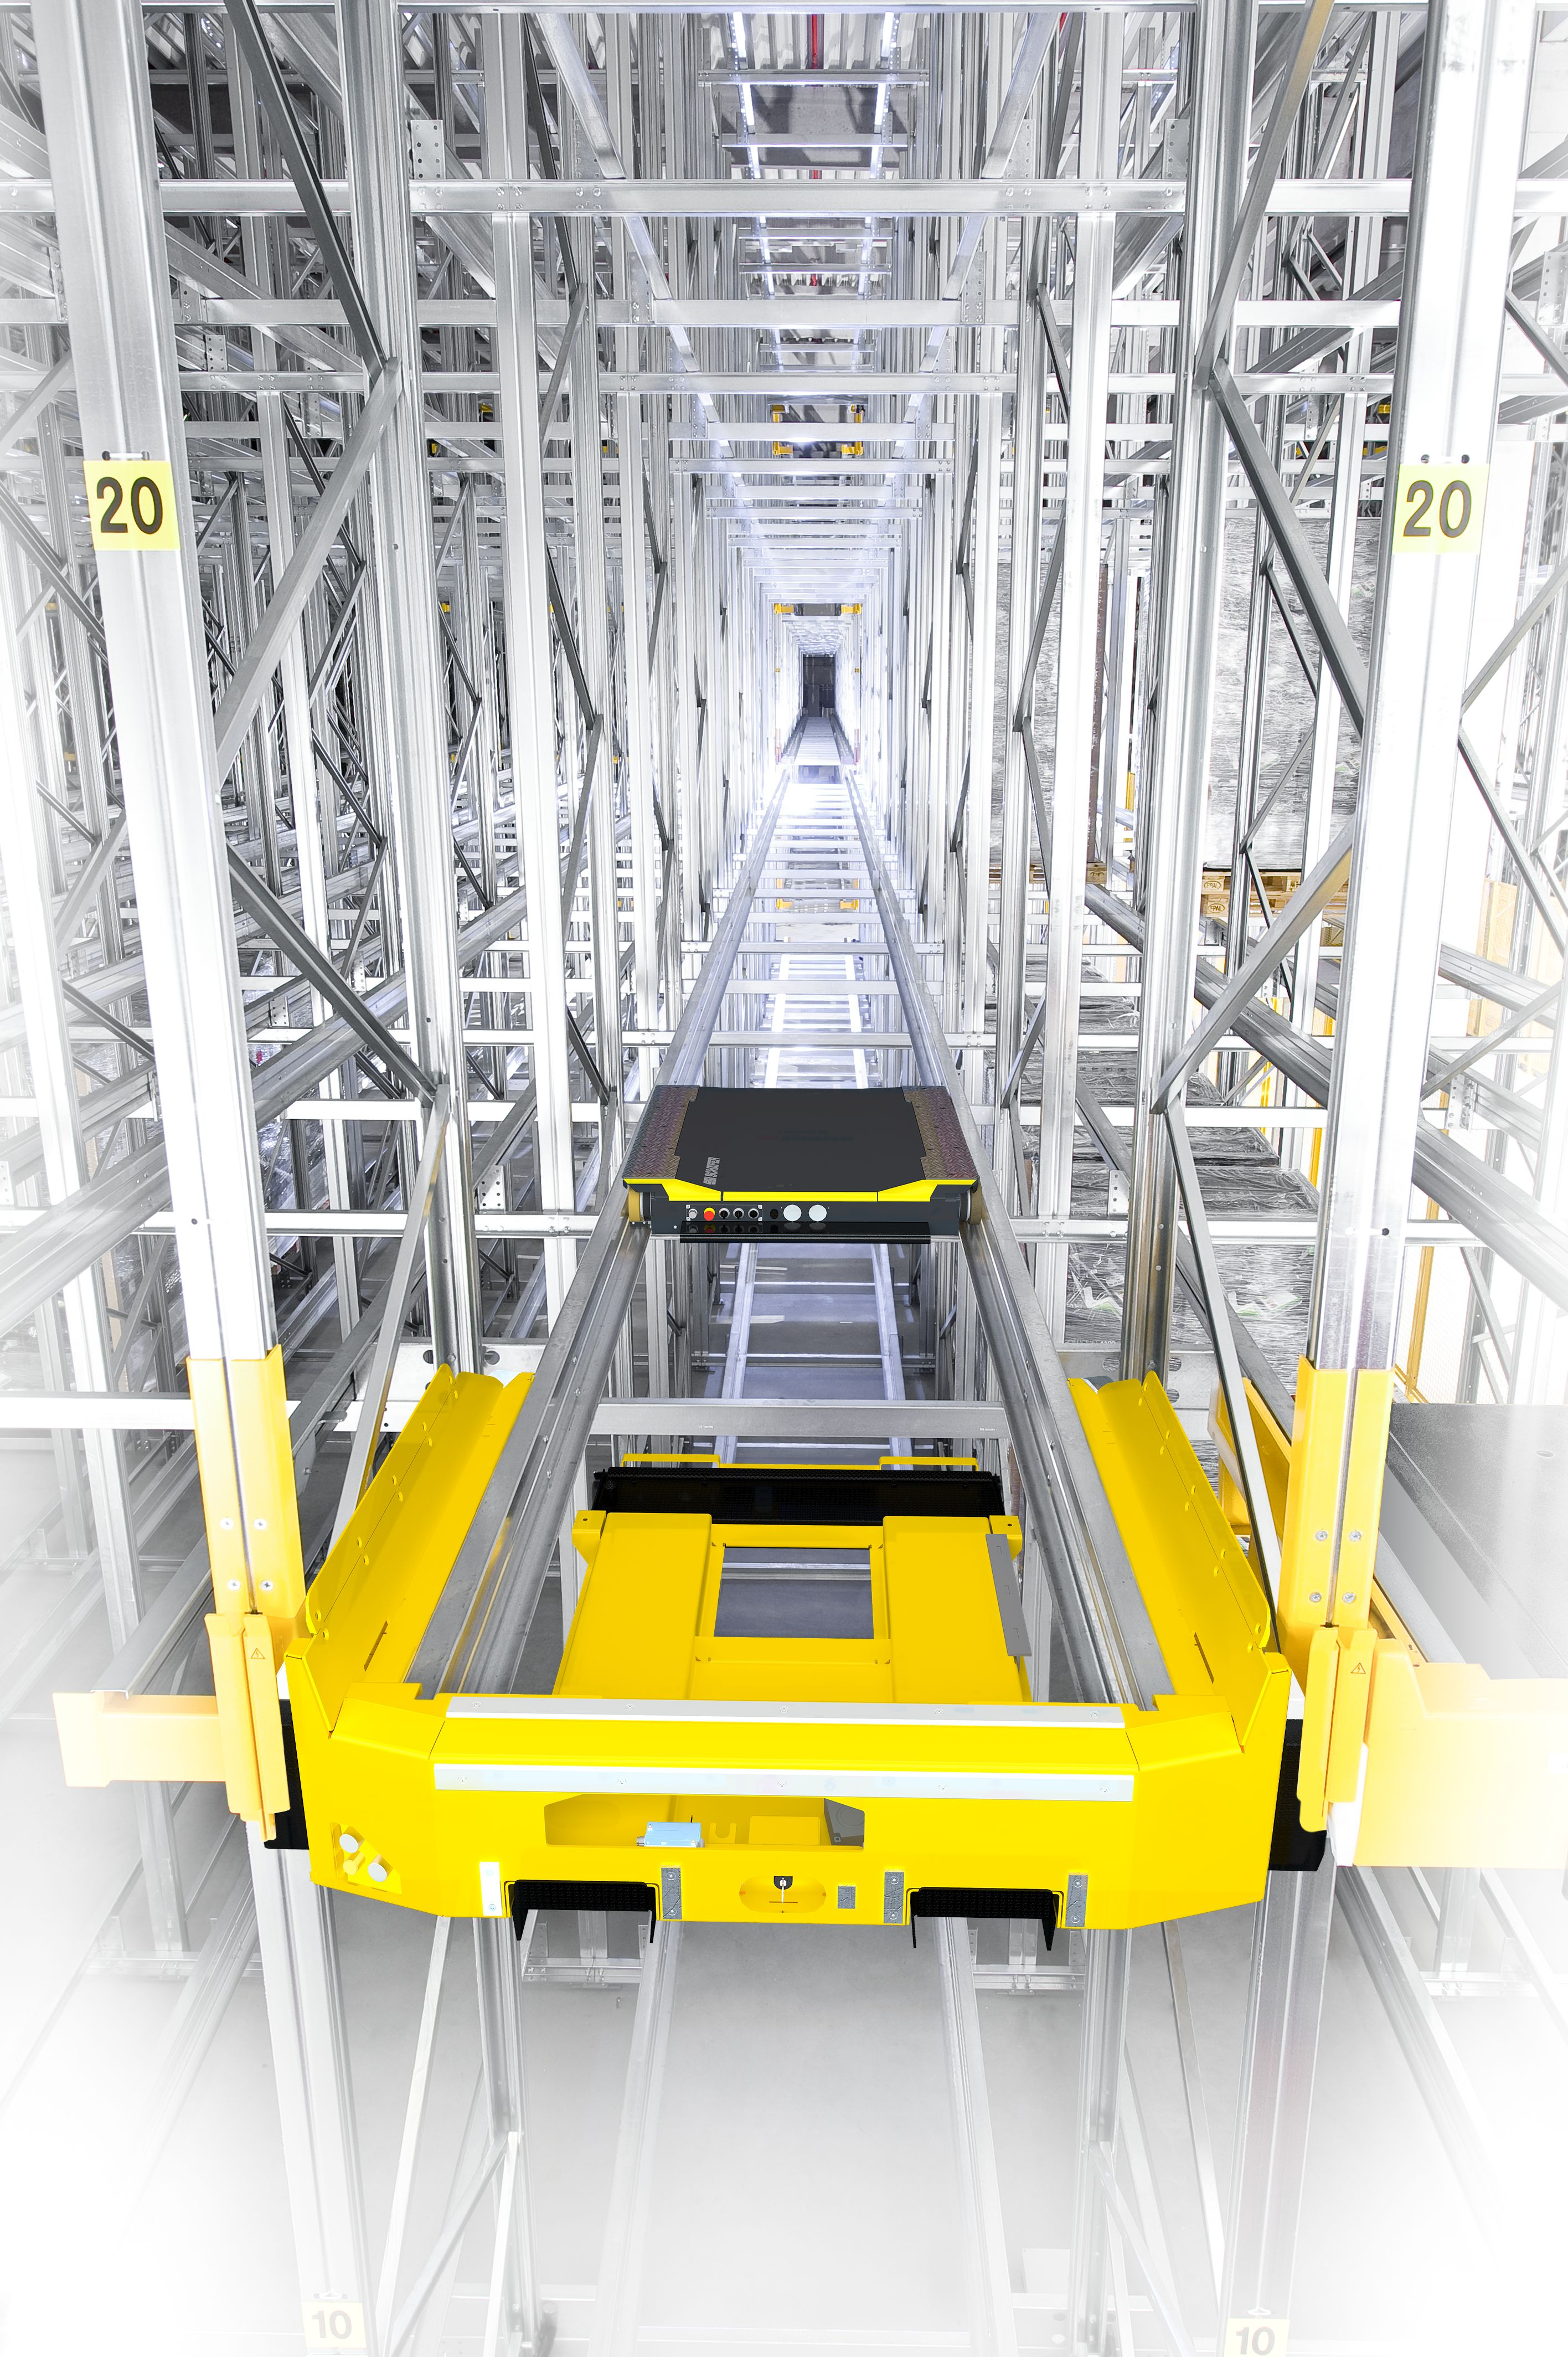
\includegraphics[width=\paperwidth,height=\paperheight]{images/ssi_orbiter_highlight.jpg}};

			\Huge
			\textbf{Mémoire de fin d'études}

			\vspace{0.5cm}
			\LARGE
			"Passer d'une application \gls{client_lourd} à une \gls{app_web} : exemple de transition d'un logiciel logistique"

			\vspace{1.5cm}

			\textbf{Anthony PINEAU}\\
			\textbf{IR2023}

			\vfill

			
\includegraphics[width=0.6\textwidth]{images/schaefer.jpg}
			\vfill
			
\includegraphics[width=0.4\textwidth]{images/esaip.jpg}

			\vfill

			Stage effectué du\\
			13 mars 2023 au 22 septembre 2023

			\vspace{0.8cm}
			
			\Large
			Maître de stage : Monsieur Thierry NEROT\\
			Tuteur pédagogique : Docteur Sofiane HAMRIOUI\\
		\end{center}
	\end{titlepage}
		
	\newpage
	\footnotesize
	\part*{Remerciements}		

		En premier lieu, je tiens à remercier Monsieur Laurent GOURDON, directeur général France de l'entreprise SSI SCHÄFER, de m’avoir permis de rejoindre à nouveau son équipe et m’avoir offert la possibilité de mettre en pratique mes connaissances et mes compétences acquises pendant mes précédentes années d’études ainsi que ces trois années du cycle ingénieur du numérique à l’ESAIP. \\

		Je tiens ensuite à remercier Monsieur Thierry NEROT, qui, en tant que maître de stage, s'est rendu disponible pour moi, et a su m'accompagner et partager ses connaissances avec moi. Il a aussi participé à la rédaction de ce mémoire en m'aidant dans la relecture et en me donnant ses conseils les plus précieux\\

		J’en profite pour remercier aussi tous les membres de l’équipe avec qui j’ai pu travailler, Messieurs Sébastien NICOD, Thibaut LUCAS et Pascal MARCELOT, qui ont su se rendre disponible pour moi si besoin. Il a d'ailleurs été très facile pour moi de pouvoir échanger avec eux et j'ai beaucoup appris auprès d'eux.\\

		Par ailleurs, je remercie également tous mes autres collègues qui ont été très accueillants tout au long du stage, Mesdames Charlotte BARGMAN, Océane SACHOT, Pauline CHAPRON, Anita BABONNEAU, Nathalie DELARUE, Roukia ATHOUMANI ainsi que Messieurs Quentin VIOLLEAU, Robin BALLON et Nicolas PERDRIAU.\\

		Je saisis cette occasion pour adresser mes profonds remerciements aux responsables et au personnel de l’ESAIP d’avoir fait le nécessaire en ce qui concerne la gestion des conventions de stage ainsi que de nous soutenir au quotidien dans notre projet pédagogique et professionnel.\\

		Je tiens ainsi à remercier tout particulièrement Monsieur Sofiane HAMRIOUI. En tant que tuteur pédagogique, nous avons pu échanger tout au long de mon stage, parler de l’avancement du projet sur lequel j'ai travaillé ainsi que travailler sur les différentes parties de ce présent mémoire.\\

		Ensuite je tiens à adresser un grand merci à ma famille, sans qui tout cela ne serait pas possible. Merci pour leurs conseils ainsi que leur soutien inconditionnel, à la fois moral et économique. Ils m’accompagnent et me soutiennent au quotidien aussi bien dans mon projet pédagogique que dans mon projet professionnel et sont une source d’inspiration pour moi.\\

		Enfin je tiens à adresser un profond remerciement à ma compagne, Madame Antonia HAMMER, pour son soutien tout au long de mon stage, et pour son aide pour la rédaction des parties en allemand de ce présent mémoire ainsi que pour la préparation de la partie allemande de la soutenance. Vielen Dank meine Liebe.

		\vspace{\baselineskip}\vspace{\baselineskip}\vspace{\baselineskip}
		\noindent
		Anthony PINEAU

	\newpage

	\normalsize
	
	%\doublespacing
	\tableofcontents

	\vspace{\baselineskip}
	\noindent Nombre de caractères totaux (hors glossaire, annexes et résumés; inclus les parties en langues étrangères) : 131 525 caractères\\
	Nombre de caractères en anglais (hors annexes et résumé) : 11 479 caractères\\
	Nombre de caractères en allemand (hors annexes et résumé) : 13 236 caractères\\

	\newpage
	
	\setcounter{page}{12}
	\renewcommand\thepage{\arabic{page}}
	\rfoot{Page \thepage}
	
	\phantomsection
	\listoffigures
	\addcontentsline{toc}{part}{\listfigurename}
	
	%\newpage

	\phantomsection
	\listoftables
	\addcontentsline{toc}{part}{\listtablename}
	\newpage

	\phantomsection
	\printglossary
	\addcontentsline{toc}{part}{\glossaryname}

	\newpage
	
	%\singlespacing

	\phantomsection
	\part*{Einleitung\footnote{Retrouver la traduction en français de la section Introduction en Annexe \ref{appendix:introduction_translation} \nameref{appendix:introduction_translation}.\\ Références utilisées pour l'aide à la rédaction de certaines parties du mémoire \cite{scribbr:remerciements}\space\cite{scribbr:introduction}\space\cite{scribbr:plan}\space\cite{scribbr:cadre_theorique}.} (Introduction)}
	%\addcontentsline{toc}{part}{Einführung (Introduction)}
		In der sich ständig verändernden, digitalen Landschaft passen sich Softwareentwicklungsansätze kontinuierlich an die, sich ständig ändernden, Benutzeranforderungen und technologischen Fortschritte an. Mit dem  Übergang von traditionellen Thick-Client-Anwendungen zu webbasierten Lösungen hat ein großer Wandel stattgefunden. Der Aufstieg des Internets und die Verbreitung von Webtechnologien haben Entwickler dazu ermutigt, die Möglichkeiten und Vorteile der Erstellung von Webanwendungen aus vorhandenen Thick-Client-Anwendungen zu erkunden.\\

		Diese Arbeit untersucht die Hauptbestandteile des komplexen Prozesses der Entwicklung einer Webanwendung aus einem bereits vorhandenen Thick Client. Ihr Ziel ist es, Entwicklern ein Beispiel für den Übergang von einer umfangreichen Client-Anwendung zu einer Webanwendung zu geben, indem ich das Projekt beschreibe, das ich während meines Abschlusspraktikums durchgeführt habe, sowie den Transformationsprozess genauer erläutere. Die Diskussion befasst sich mit den Herausforderungen, Methoden und geeigneten Vorgehensweisen, die mit dieser Transformation verbunden sind, und ermöglicht es Softwareentwicklern, die Feinheiten des Entwicklungsprozesses erfolgreich zu meistern.\\

		Während meines Abschlussprojekts hatte ich die Möglichkeit, an der Gestaltung einer Webanwendung mitzuwirken, die aus einer Thick-Client-Anwendung entstand. Dieser Ansatz zielt darauf ab, die Bereitstellung zu beschleunigen und die Ästhetik der Benutzeroberfläche zu modernisieren. Diese Erfahrung motivierte mich, mein Verständnis für den Prozess der Entwicklung von Webanwendungen zu vertiefen, die aus Thick-Client-Anwendungen entstehen.\\
		
		Typischerweise besteht eine Webanwendung im Wesentlichen aus zwei Hauptkomponenten: dem \Gls{frontend}, das sich auf die, für den Benutzer wahrnehmbare grafische Oberfläche bezieht, und dem \Gls{backend}, das den Zugriff auf die Datenbank und die Verarbeitung von Datenanfragen verwaltet. In diesem speziellen Szenario wird unsere Anwendung erstellt,  indem ein bestimmter Teil für die Benutzeroberfläche abgetrennt wird, die über HTTP-Anfragen mit einer \acrshort{rest}-\acrshort{api} interagiert. Diese \acrshort{api} fungiert als Kommunikationsverbindung mit der Datenbank.\\
		
		Dieses Dokument beschreibt die Überlegungen zum Design einer Webanwendung, die von einer Thick-Client-Anwendung abgeleitet wird. Wir werden mehrere Elemente abdecken, darunter die Wahl der Programmiersprache und des \Glspl{framework} sowie die vollständige Implementierung der Anwendung, einschließlich der Erstellung der grafischen Oberflächen.\\
		
Um sich mit dem Thema auseinanderzusetzen und Antworten auf die aufgeworfenen Fragen zu geben, wurde ein Forschungsplan entwickelt. Zunächst galt es, eine fundierte Entscheidung bezüglich der Programmiersprache zu treffen und so eine solide Grundlage zu schaffen. Als nächstes wurde an der Erstellung einer neuen grafischen Oberfläche gearbeitet. Zum Abschluss des Prozesses wurde die Integration mit der Datenbank über eine \acrshort{rest}-\acrshort{api} implementiert.\\
		
		Das Ziel der Studie besteht darin, den Prozess der Erstellung einer Webanwendung aus einem umfangreichen Kundenstamm zu verstehen und gleichzeitig die Hauptunterschiede zwischen diesen beiden Ansätzen zu identifizieren.\\
		
		Zu Beginn dieser Dissertation beginnen wir mit einer Präsentation des Unternehmens, das mich willkommen geheißen hat, nämlich SSI SCHÄFER. Als nächstes werden wir den theoretischen Rahmen festlegen, der für das Verständnis der, in diesem Dokument beschrieben, Schlüsselkonzepte unerlässlich ist. Anschließend wenden wir uns dem wissenschaftlichen Teil zu, der sich auf eine vergleichende Analyse zwischen Thick-Client-Anwendungen und Webanwendungen konzentriert.\\

		Danach werden wir uns mit dem Kern des Projekts befassen, es  im Detail vorstellen und gleichzeitig seine Probleme und seine Bedeutung  hervorheben. Es folgt ein ausführlicher Überblick über die Methodik und die Tools, die zum Erfolg des Projekts beigetragen haben. Anschließend beschreiben wir den Verlauf des Projekts, stellen die verschiedenen durchgeführten Phasen dar und besprechen die aufgetretenen Herausforderungen, die erzielten Erfolge sowie die während dieser Praktikumszeit erzielten Ergebnisse.\\

		Bevor wir zum Abschluss kommen, ziehen wir eine Bilanz der in den letzten sechs Monaten erworbenen und entwickelten Fähigkeiten. Abschließend finden Sie im Anhang zusätzliche Informationen, gefolgt von einer Zusammenfassung der Dissertation in drei Sprachen: Französisch, Englisch und Deutsch.

	\newpage

	%glossaire
	%\gls{latex}
	%\Glspl{formula} première lettre majuscule et pluriel
	
	%acronyme
	%\acrlong{wms}
	%\acrshort{wms}
	%\acrfull{wms}
		
		\part{Contexte global\footnote{Références utilisées dans la partie \ref{section:context} Contexte global : \cite{schaefer}\space\cite{schaeferHistory}\space\cite{schaeferFR}\space\cite{schaeferMorpheus}\space.}}\label{section:context}
		Dans le cadre de ce mémoire, il est essentiel de comprendre le contexte global dans lequel l'entreprise SSI SCHÄFER évolue. Ainsi dans cette section, nous allons découvrir l'histoire de l'entreprise ainsi que les produits et services qu'elle propose. Nous reviendrons aussi suite la suite logicielle Morpheus qui sera au c\oe ur de ce document. \gls{API}
		
		\section{L'entreprise : SSI SCHÄFER}
			L'entreprise SSI SCHÄFER est aujourd'hui l'un des premiers fournisseurs mondiaux de produits et systèmes logistiques pour le stockage, la préparation des commandes et la gestion des déchets. Ces solutions intralogistiques, partiellement ou entièrement automatisées, permettent d’optimiser les flux logistiques et l’aménagement des entrepôts et centres logistiques de nos clients, peu importe leur surface de stockage et leur secteur d’activité.

			\begin{figure}[h!]
				\begin{center}
					
\includegraphics[width=0.7\linewidth]{images/schaefer.jpg}
				\end{center}
				\caption{Logo de l'entreprise SSI SCHÄFER}
				\floatfoot{Source de l'image : \url{https://www.ssi-schaefer.com/resource/crblob/480/a14c9a665a8272cc2b80687168a2e3d7/logo-ssi-schaefer-svg-data.svg}}
				\label{fig:schaefer}
			\end{figure}	
			\newpage
			\subsection{Histoire}
				C'est en 1935 que Fritz SCHÄFER (1893-1951) commença à construire ses premiers conteneurs de transport, pendant son temps libre, dans l'espace minuscule de sa propre buanderie. Deux ans plus tard, le plombier et soudeur de formation réalise son rêve et fonde son entreprise pour produire des « produits et articles en tôle ». L'entreprise a été officiellement enregistrée à Burbach, en Allemagne, le 16 janvier 1937. Elle connaît un succès immédiat et doit dès 1939 construire son premier grand hall de production.\\

				La société s'internationalise au début des années 1960 avec la création de filiale en Suisse et en Angleterre. En 1965, Fritz SCHÄFER commence désormais la production de rayonnages à étagères et à palettes. L'entreprise se diversifie à l'aube du deuxième millénaire avec la création de SSI SCHÄFER Noell et SSI SCHÄFER Peem qui proposent des prestations avec des solutions d'automatisation. C'est en 2005 que les trois entreprises se regroupent sous la marque SSI SCHÄFER.\\

				En 2008, le spécialiste logiciel, Salomon Automation, rejoint l'entreprise. Puis SSI SCHÄFER rachète l'entreprise danoise Handler A/S, expert en tours de stockage, en 2010. 2017 est un nouveau tournant pour l'entreprise avec la création de SSI SCHÄFER IT SOLUTIONS GMBH et une nouvelle dénomination sociale SSI SCHÄFER AUTOMATION GMBH.\\
			
				Vous pourrez par ailleurs trouver en annexes \ref{appendix:history} \nameref{appendix:history} et \ref{appendix:map} \nameref{appendix:map} une frise historique avec les dates importantes de l'histoire SSI SCHÄFER ainsi que la carte de toutes les filiales de l'entreprise.

			\newpage

			\subsection{SSI SCHÄFER en France}
				Le groupe SSI SCHÄFER est représenté par deux filiales en France, qui couvrent l'ensemble du territoire français et des besoins intralogistiques.\\

				Créée en 1963, SSI SCHAEFER SAS a son siège en historique en Moselle, on y retrouve notamment toutes les fonctions administratives et de soutien stratégique ainsi que la conception. Les commerciaux et techniciens de maintenance sont déployés sur l'ensemble du territoire français, ce qui garantit une proximité avec les clients et des temps de réaction brefs dans toute la France.\\

				En automne 2017, SSI SCHÄFER fait l'acquisition de GRN Logistic, basé à Cholet, qui vient compléter, par son expertise dans le domaine des logiciels logistiques, l'expérience nationale et internationale du groupe dans la vente de solutions intralogistiques. Ce qui vient améliorer la compétence globale de SSI SCHÄFER en France.
			
			\subsection{Solutions intralogistiques}
				SSI SCHÄFER élabore, conçoit et fabrique des systèmes intralogistiques modulaires, destinés à tous les besoins en stockage, préparation de commandes et convoyage :
				\begin{itemize}
					\bdot{Solutions de stockage}
						\begin{itemize}
							\bdotoutlined{Rayonnage tous types}
							\bdotoutlined{Bacs et conteneurs}
							\bdotoutlined{Tours de stockage}
							\bdotoutlined{Trans-stockeurs}
							\bdotoutlined{Navettes}
							\bdotoutlined{Orbiters}
						\end{itemize}
					\bdot{Solutions de convoyage}
						\begin{itemize}
							\bdotoutlined{Convoyeur de bacs, cartons, palettes et plateaux}
							\bdotoutlined{Convoyeur aérien}
							\bdotoutlined{Système de transport sans conducteurs (AGVs)}
						\end{itemize}
					\bdot{Systèmes de préparation de commandes}
						\begin{itemize}
							\bdotoutlined{"Man to products" : pick by light, pick by voice, RF picking}
							\bdotoutlined{"Products to Man": caroussel, trieur, A-Frame, pick to tote}
							\bdotoutlined{Tours de stockage et rayonnages dynamiques}
						\end{itemize}
					\bdot{Solutions clefs en main}
						\begin{itemize}
							\bdotoutlined{Planification logistique globale et conseil}
							\bdotoutlined{Construction des bâtiments et installations}
							\bdotoutlined{Prestations de service et de maintenance sur mesure}
						\end{itemize}
				\end{itemize}

			\begin{figure}[h!]
				\begin{center}
					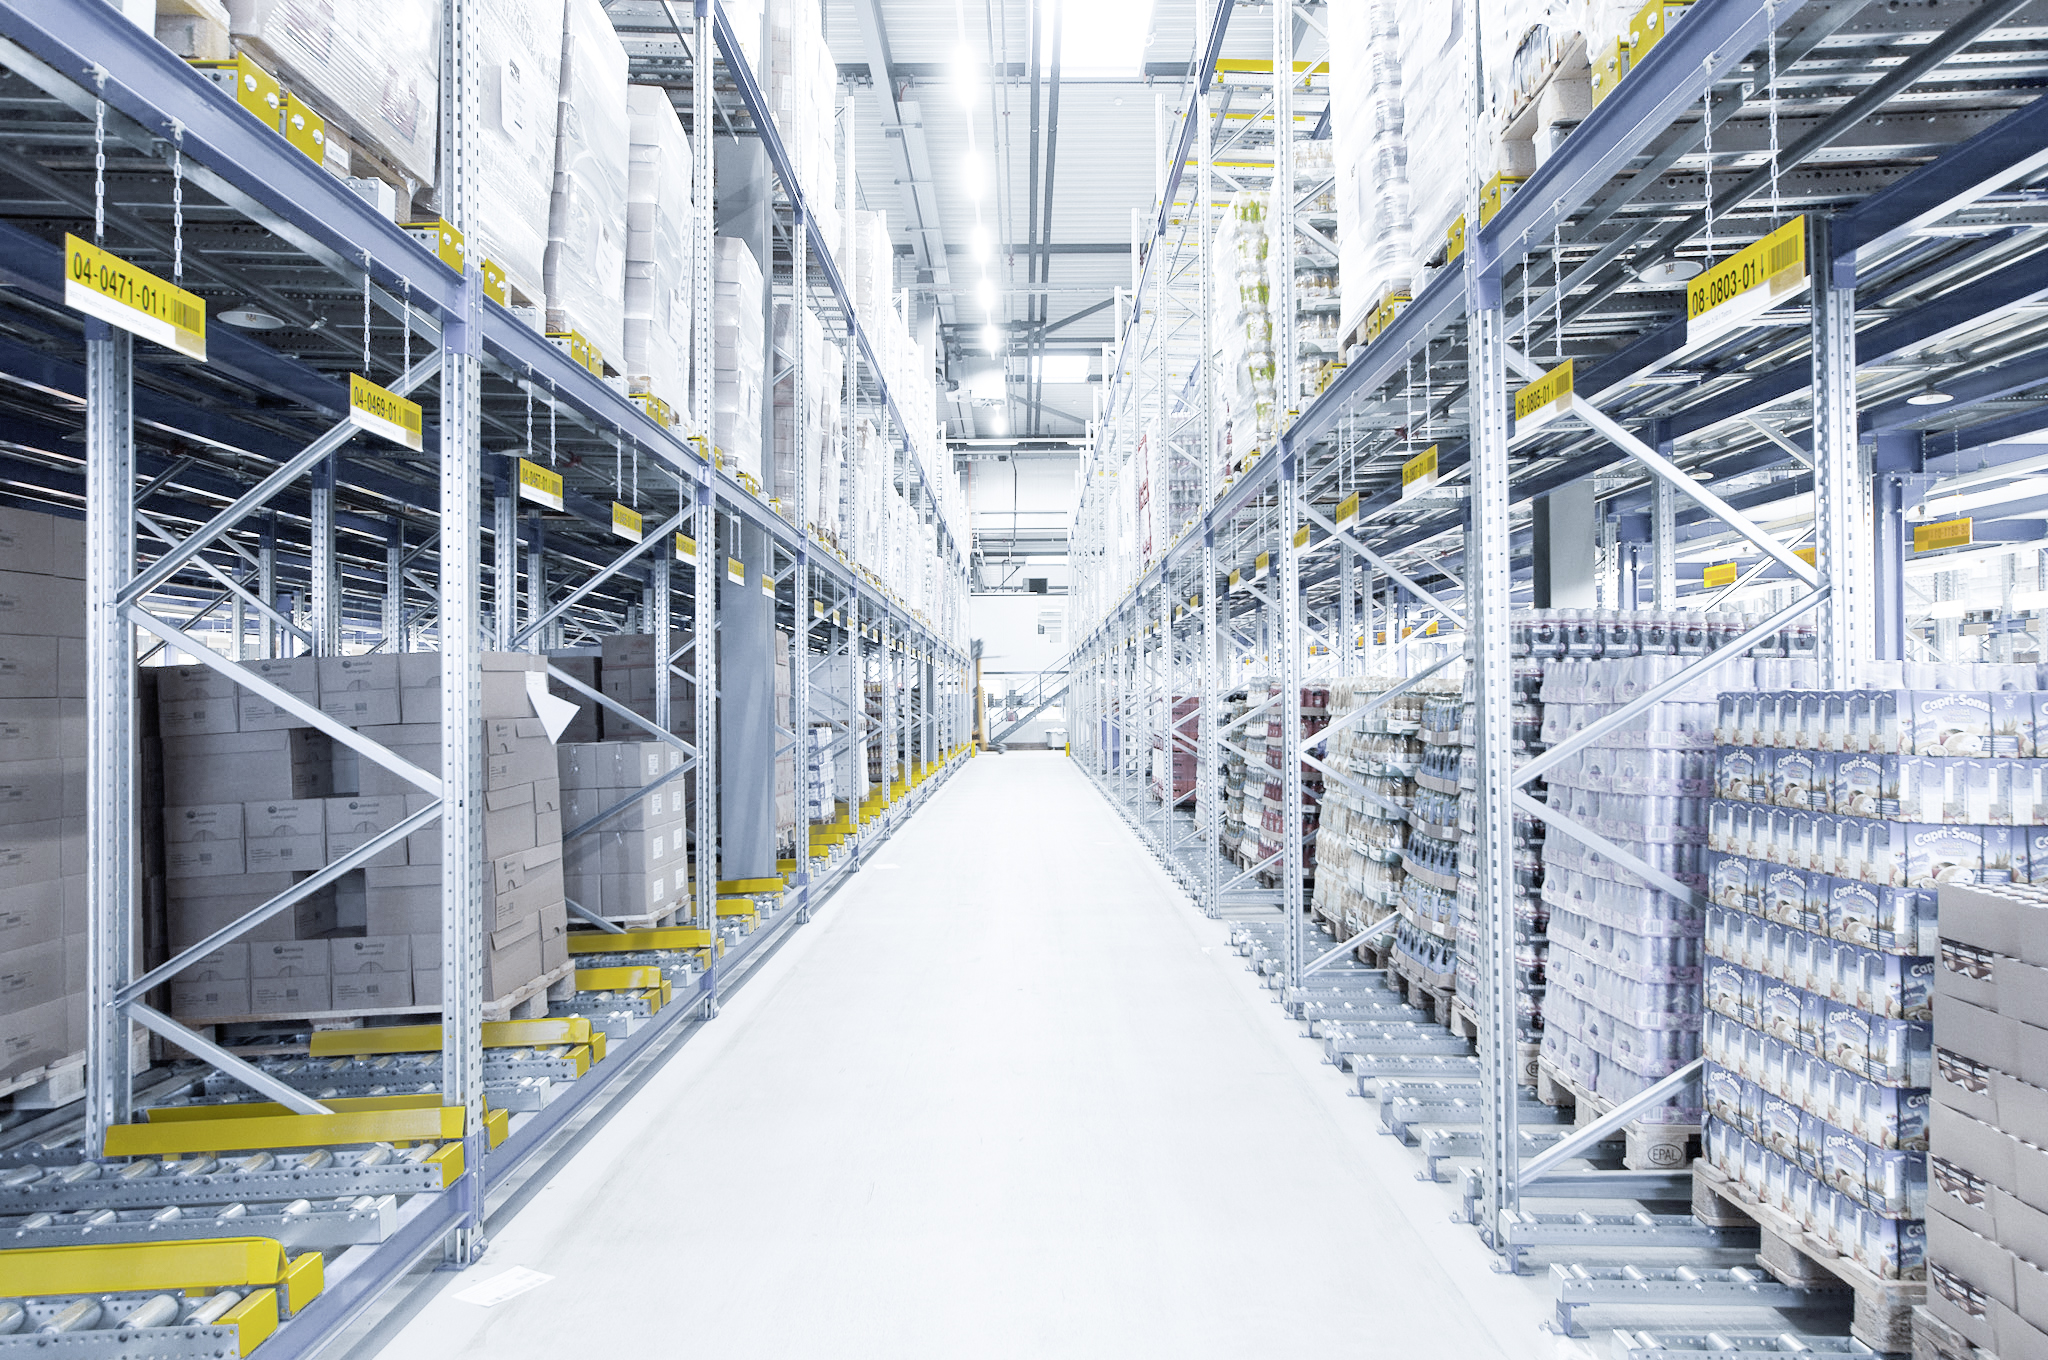
\includegraphics[width=0.7\linewidth]{images/intralogistic.jpg}
				\end{center}
				\caption{Exemple de solution intralogistique}
				\floatfoot{Source de l'image : base de données d'images interne de l'entreprise}
				\label{fig:intralogistic}
			\end{figure}
			\newpage
			\subsection{Solutions logicielles}
				Les processus intralogistiques sont de plus en plus complexes. Dans les entrepôts manuels, automatisés et entièrement automatisés, d'innombrables processus doivent être contrôlés, visualisés et optimisés. Cela exige de l'expertise. En tant que premier fournisseur mondial de systèmes logistiques, SSI SCHÄFER ne se contente pas de proposer tout ce dont on a besoin pour des entrepôts, mais propose également l'expertise informatique.\\

				\noindent
				Exemples de logiciels logistiques développés par SSI SCHÄFER :
				\begin{itemize}
					\bdot{WAMAS}
					\bdot{MORPHEUS}
				\end{itemize}
				\vspace{\baselineskip}
				\par Nous nous intéresserons ici à MORPHEUS, logiciel développé en France par GRN Logistics, avec lequel j'ai travaillé durant mon stage.
		
		\section{MORPHEUS}
				La suite logicielle MORPHEUS est une gamme de logiciels dédiée à la gestion et à l'optimisation de la performance de la logistique. Elle est composée de différents modules :
			\begin{itemize}
				\bdot{\gls{WMS} Gestion des entrepôts}
				\bdot{\gls{WCS} Pilotage de stockeurs et de préparation de commandes automatisés}
			\end{itemize}

			\subsection{Morpheus \acrshort{wms}}
				\noindent				
				Les objectifs du WMS :%paragraph ?
				\begin{itemize}
					\bdot{Augmenter votre productivité}
					\bdot{Réduire les stocks}
					\bdot{Optimiser les surfaces de stockages}
					\bdot{Diminuer les erreurs}
				\end{itemize}
				\newpage
				\noindent Quelques fonctionnalités du WMS :
				\begin{itemize}
					\bdot{Moteur de règles pour la gestion des stratégies métiers}
					\bdot{Planification et pré-réception}
					\bdot{Création et affectation automatique des emplacements}
					\bdot{Ordonnancement manuel et automatique}
					\bdot{Pilotage des ressources humaines}
				\end{itemize}
			
			\subsection{Morpheus \acrshort{wcs}}
				\noindent
				Les objectifs du WCS :
				\begin{itemize}
					\bdot{Mécaniser et automatiser les flux}
					\bdot{Intégrer et synchroniser les WMS \& WCS}
					\bdot{Séquencez l'activité des équipements}
					\bdot{Superviser et optimiser les process}
				\end{itemize}
				\vspace{\baselineskip}
				Quelques fonctionnalités du WCS :
				\begin{itemize}
					\bdot{Pilotage de convoyeurs pour le transport de cartons, bacs...}
					\bdot{Pilotage du stockage et de la préparation de commandes}
					\bdot{Pilotage des trieurs / robots / meubles de tri}
				\end{itemize}
				\vspace{\baselineskip}
				Retrouvez plus d'informations sur le WMS et le WCS en annexe \ref{appendix:morpheusWMSFonctionnalites} \nameref{appendix:morpheusWMSFonctionnalites} et \ref{appendix:morpheusWCSFonctionnalites} \nameref{appendix:morpheusWCSFonctionnalites}

	\newpage

	\part{Cadre théorique}
		Le cadre théorique est un pilier fondamental de tout projet ou étude, car il offre la base conceptuelle nécessaire à la compréhension et à la contextualisation de tout travail. Dans cette section, nous allons explorer les théories et les concepts les plus importants pour bien comprendre le projet.\\

		Vous pourrez également trouver de nombreuses définitions dans le glossaire, la plupart d'entre elles étant des termes techniques, mais moins importantes.
			
		\section[Application \gls{client_lourd}]{\printSectionFootnote{subsection:cadre_theorique:application_client_lourd}{wikipedia:client_lourd}}\label{subsection:cadre_theorique:application_client_lourd}
			Un logiciel \gls{client_lourd} offre des fonctionnalités complexes avec une capacité de traitement autonome. Le terme "client" est lié à l'architecture client-serveur. Contrairement au \gls{client_leger}, le \gls{client_lourd} dépend principalement du serveur pour l'échange de données, mais il assume habituellement la totalité du traitement.

		\section[\Gls{app_web}]{\printSectionFootnote{subsection:cadre_theorique:application_web}{wikipedia:application_web}}\label{subsection:cadre_theorique:application_web}
			Dans le domaine informatique, une \gls{app_web} (également désignée sous le terme web application) est une application qui peut être utilisée directement via un navigateur web\footnote{Le navigateur web est un \gls{client_leger}}, sans nécessiter une installation sur les dispositifs utilisateurs, contrairement aux applications \gls{client_lourd}. De manière similaire aux sites web, une \gls{app_web} est généralement hébergée sur un serveur et peut être contrôlée en interagissant avec des éléments interactifs via un navigateur web, en exploitant un réseau informatique (comme Internet, un intranet ou un réseau local).
				
		\newpage
		\section[\Gls{frontend} et \gls{backend}]{\printSectionFootnote{subsection:cadre_theorique:frontend_backend}{wikipedia:frontend_backend}}\label{subsection:cadre_theorique:frontend_backend}
			En génie logiciel, les termes "\gls{frontend}" et "\gls{backend}" font référence à la séparation des préoccupations entre la couche de présentation (\gls{frontend}) et la couche d'accès aux données (\gls{backend}) d'un logiciel. Dans le modèle client-serveur, le client est généralement considéré comme le \gls{frontend} et le serveur comme le \gls{backend}, même lorsque certaines tâches de présentation sont effectivement réalisées sur le serveur lui-même.			
			
		\section[\Gls{framework}]{\printSectionFootnote{subsection:cadre_theorique:framework}{wikipedia:framework}}\label{subsection:cadre_theorique:framework}
			En programmation informatique, un \gls{framework} représente un ensemble cohérent de composants logiciels structurels qui servent à établir les bases ainsi que les contours généraux d'une partie ou de l'ensemble d'un logiciel, en d'autres termes, son architecture. Ce qui distingue un \gls{framework} d'une simple \gls{bibliotheque_logicielle}, c'est principalement, d'une part, sa nature générique et sa faible spécialisation, contrairement à certaines \gls{bibliotheque_logicielle}s. Un \gls{framework} peut être composé de plusieurs bibliothèques logicielles, chacune ayant une spécialisation dans un domaine particulier. Néanmoins, un \gls{framework} peut aussi être spécialisé dans un langage spécifique, une plateforme particulière, ou un domaine spécifique, comme la communication de données ou le mappage de données. D'autre part, il impose un cadre de travail inhérent à sa propre structure, ce qui guide l'architecture logicielle voire encourage le développeur à suivre certains modèles de conception. Les \gls{bibliotheque_logicielle}s à l'intérieur du \gls{framework} sont organisées selon le même paradigme.

		\newpage
		\section[\acrshort{api} : \gls{API}]{\printSectionFootnote{subsection:cadre_theorique:api}{wikipedia:api}}\label{subsection:cadre_theorique:api}
			En informatique, une interface de programmation d'application, également connue sous le nom d'interface de programmation applicative (\acrshort{api}), souvent abrégée en \acrshort{api} pour "application programming interface", constitue un ensemble normalisé de classes, de méthodes, de fonctions et de constantes servant de façade par laquelle un logiciel propose des services à d'autres logiciels. Celle-ci est fournie par une \gls{bibliotheque_logicielle} ou un service web, généralement accompagnée d'une description qui détaille comment les programmes "consommateurs" peuvent tirer parti des fonctionnalités du programme "fournisseur".

		\section[\acrshort{rest} : \gls{REST}]{\printSectionFootnote{subsection:cadre_theorique:rest}{wikipedia:rest}}\label{subsection:cadre_theorique:rest}
			\acrshort{rest} (\gls{REST}) représente un style d'architecture logicielle qui énonce un ensemble de directives à suivre pour la création de services web. Les services web qui adhèrent à l'architecture \acrshort{rest}, également appelés services web \acrshort{rest}ful, établissent une communication interopérable entre les ordinateurs connectés sur Internet. Ces services web \acrshort{rest} autorisent les systèmes qui effectuent des requêtes à interagir avec des ressources en ligne par le biais de leurs représentations textuelles, en utilisant un ensemble uniforme et prédéfini d'opérations, sans état. En opposition, d'autres types de services web tels que les services web SOAP présentent leurs propres ensembles d'opérations variées.\\

			Grâce à l'utilisation d'un protocole sans état et d'opérations standardisées, les systèmes \acrshort{rest} visent la réactivité, la fiabilité et l'extensibilité, en permettant la réutilisation de composants qui peuvent être gérés et mis à jour sans perturber le fonctionnement global du système, même pendant son exécution.
	
	\newpage
	\phantomsection
	\part{Partie scientifique : analyse comparative des applications \gls{client_lourd} et des \glspl{app_web} \footnote{Références utilisées dans la partie \ref{part:scientific} Partie scientifique : analyse comparative des applications \gls{client_lourd} et des \glspl{app_web} : \cite{wikipedia:client_leger}\space\cite{wikipedia:client_lourd}\space\cite{wikipedia:application_web}\space\cite{wikipedia:acces_internet}\space\cite{wikipedia:internet}\space\cite{wikipedia:plateforme_client_riche}\space\cite{wikipedia:client_informatique}\space\cite{scientific:app_master}\space\cite{scientific:eposaudio}\space\cite{scientific:journal_net}\space\cite{scientific:profolus}\space\cite{scientific:audiviklabs}\space\cite{scientific:minnalearn}\space\cite{scientific:cyberpreventys}\space\cite{scientific:techtarget}\space\cite{scientific:techgenix}\space\cite{scientific:baeldung}\space\cite{scientific:ionos_client_lourd}\space\cite{scientific:agence_scroll}\space\cite{scientific:yeeply}\space\cite{scientific:digitiz}\space\cite{scientific:hicones}\space\cite{scientific:yourstory}\space\cite{scientific:ionos_client_leger}\space\cite{scientific:proofpoint}\space\cite{scientific:bluemind}.}}\label{part:scientific}
		Afin d'établir des bases solides pour l'étude, cette section réalisera une analyse comparative approfondie des caractéristiques et des fonctionnalités des applications \gls{client_lourd} par rapport aux \glspl{app_web}. En comprenant les forces et les faiblesses des deux approches, les développeurs acquerront des informations cruciales sur les défis et les opportunités qui les attendent lors du processus de transformation.
		
		\section{Introduction}
			Au cours de cette analyse, nous allons explorer en profondeur les différences fondamentales entre les applications \gls{client_lourd} et les \glspl{app_web}. Nous examinerons leurs performances, leurs capacités d'accessibilité, leur sécurité ainsi que leur convivialité. En mettant en évidence les forces et les faiblesses de chaque approche, nous serons en mesure d'évaluer les cas d'utilisation optimaux pour chaque type d'application.
			
			\subsection{Présentation du sujet}
				L'essor de la technologie a donné lieu à une diversification des plateformes logicielles, dont les applications \gls{client_lourd} et les \glspl{app_web}, qui offrent des expériences utilisateur distinctes. Cette analyse comparative se penche sur ces deux approches de développement logiciel, mettant en évidence leurs avantages, inconvénients et domaines d'application respectifs. En examinant les caractéristiques techniques, les performances, la convivialité et d'autres aspects clés, cette étude vise à fournir un aperçu approfondi des forces et des faiblesses des applications \gls{client_lourd} et des \glspl{app_web}.
			
			\subsection{Contexte de l'analyse}
				L'analyse comparative des applications \gls{client_lourd} et des \glspl{app_web} concerne l'évaluation des avantages et des inconvénients de ces deux types d'applications informatiques. Les applications client lourd et les \glspl{app_web} sont deux approches différentes pour fournir des logiciels et des services aux utilisateurs. Ici l'analyse n'a pas pour but de dire quelle méthode est la meilleure mais de comparer deux façons de faire et de voir dans quels scénarios il peut être plus intéressant d'utiliser l'un ou l'autre.
			
			\subsection{Énoncé de la problématique}		
				Face à la diversité croissante des besoins en matière de logiciels interactifs, comment choisir de manière éclairée entre le développement d'applications \gls{client_lourd} et d'\glspl{app_web} ? Quels sont les facteurs décisifs, tels que les performances, la sécurité, l'accessibilité et l'expérience utilisateur, qui devraient guider cette décision pour répondre au mieux aux besoins des utilisateurs et aux objectifs des développeurs ? Cette analyse comparative vise à éclairer les avantages et les inconvénients de chaque approche, afin de fournir des recommandations éclairées pour le choix optimal entre applications \gls{client_lourd} et \glspl{app_web} en fonction de différents contextes et exigences.
	
			\subsection{Résumé}
				L'objectif ici n'est donc pas de déterminer la supériorité entre les applications \gls{client_lourd} et les \glspl{app_web}, mais plutôt d'analyser les diverses situations dans lesquelles l'une pourrait s'avérer plus avantageuse que l'autre. Cette démarche nous permettra également de saisir les raisons qui nous ont poussés à développer une \gls{app_web} dérivée du client Morpheus.				

		\newpage
		\section{Définitions et concepts de base}
			\subsection{Explication des applications \gls{client_lourd}}
				Un logiciel \gls{client_lourd} offre des fonctionnalités complexes avec une capacité de traitement autonome. Le terme "client" est lié à l'architecture client-serveur. Contrairement au \gls{client_leger}, le \gls{client_lourd} dépend principalement du serveur uniquement pour l'échange de données et assume habituellement la totalité du traitement. Les applications \gls{client_lourd} sont des logiciels installés et exécutés localement sur l'ordinateur de l'utilisateur. Elles offrent généralement une expérience riche en fonctionnalités et en performances, car elles peuvent tirer parti des ressources locales de l'ordinateur, telles que la puissance de traitement et la mémoire.
			
			\subsection{Explication des \glspl{app_web}}
				Dans le domaine informatique, une \gls{app_web} (également désignée sous le terme web application) est une application qui peut être utilisée directement via un navigateur web, sans nécessiter une installation sur les dispositifs utilisateurs, contrairement aux applications mobiles. De manière similaire aux sites web, une \gls{app_web} est généralement hébergée sur un serveur et peut être contrôlée en interagissant avec des éléments interactifs via un navigateur web, en exploitant un réseau informatique (comme Internet, un intranet ou un réseau local). Elles ne nécessitent donc pas d'installation locale et offrent une approche plus flexible pour l'accès aux logiciels et aux services.
			
			\subsection{Discussion sur la connectivité internet et son rôle dans les \glspl{app_web}}
				Internet est un réseau informatique planétaire accessible au grand public. C'est un assemblage de réseaux, fonctionnant par commutation de paquets, dépourvu de point central, qui rassemble des millions de réseaux variés, qu'ils soient publics ou privés, universitaires, commerciaux ou gouvernementaux. Tous ces réseaux sont regroupés en entités autonomes. L'accès à Internet fait référence aux moyens fournis afin de se connecter à la toile mondiale, Internet.

				La conception et l'utilisation d'applications directement sur le Web offrent la possibilité de reproduire l'expérience d'un logiciel traditionnel depuis le navigateur, en mettant à disposition des fonctionnalités autrefois exclusives aux environnements des ordinateurs individuels. Cela permet aux utilisateurs de bénéficier d'un accès uniforme aux mêmes fonctionnalités à travers différents dispositifs.
		
		\section{Avantages des applications \gls{client_lourd}}
			Dans le paysage numérique en constante évolution, les applications \gls{client_lourd} occupent une place importante en offrant une expérience utilisateur exceptionnelle et des fonctionnalités avancées. Contrairement aux \glspl{app_web} qui fonctionnent dans un navigateur, les applications \gls{client_lourd} sont installées localement sur l'ordinateur de l'utilisateur. Cette approche présente plusieurs avantages significatifs qui en font le choix privilégié pour de nombreuses entreprises et utilisateurs exigeants. Dans cette section, nous explorerons en détail les atouts majeurs des applications client lourd, allant des performances optimisées à la disponibilité hors ligne, en passant par la flexibilité de personnalisation.
			
			\subsection{Performances}
				L'application de bureau vous offre la possibilité d'implémenter toute sorte de fonctionnalité. Jusqu'à présent, aucun équivalent en ligne complet de logiciels tels que Photoshop ou Sony Vegas n'a été développé. Les utilitaires système demeurent principalement dans le domaine du développement de bureau. En plus des programmes destinés à fonctionner en arrière-plan sur de longues périodes, comme les chats ou les clients torrent, utiliser ces programmes via un navigateur serait tout simplement inconfortable. De plus, ces logiciels sont souvent utilisés pour des projets spécifiques, avec des interfaces ou des fonctions non conventionnelles.

				\subsubsection{Performances du serveur}
					Une architecture client-serveur qui repose sur des \glspl{client_lourd} n'exige pas des serveurs hautement performants. En effet, le traitement et d'autres fonctionnalités matérielles se produisent au niveau local ou individuel plutôt qu'à un niveau centralisé. De plus, cet atout implique que le serveur peut prendre en charge un nombre accru d'utilisateurs, ce qui se traduit par une capacité de serveur supérieure.

				\subsubsection{Performances de l'ordinateur client}
					Toute application exigeante en termes de ressources ou de bande passante doit pouvoir fonctionner de manière optimale, étant donné que les ressources proviennent des ordinateurs individuels et ne sont pas allouées par un serveur central. Les \glspl{client_lourd} sont en mesure de faire fonctionner des applications qui requièrent une quantité considérable de ressources. Par exemple, les jeux vidéo nécessitent une grande bande passante et une puissance de traitement élevée de l'ordinateur, ce qui garantit une expérience fluide, sans interruptions ni ralentissements.
			
			\subsection{Expérience utilisateur}
				\subsubsection{Interface utilisateur graphique riche}
					L'un des aspects positifs marquants des \glspl{client_lourd} réside dans leur aptitude à offrir une interface utilisateur graphique de haute qualité. Des exemples d'interfaces de ce genre englobent des systèmes d'exploitation complets, des programmes ou applications informatiques immersives, ainsi que des jeux vidéo à la forte intensité graphique. Il est important de noter que la majorité des \glspl{client_leger} ne sont pas en mesure de reproduire des graphismes sophistiqués en raison des restrictions liées aux capacités de traitement, de calcul et d'espace de stockage disponibles.
				\newpage
				\subsubsection{Possibilité de personnalisation}
					En règle générale, les \glspl{client_leger} sont administrés à distance avec une participation limitée de la part de l'utilisateur final. En revanche, les \glspl{client_lourd} peuvent être adaptés par les employés individuels grâce à l'installation des logiciels et applications requis directement au niveau local.
			
			\subsection{Fonctionnalités avancées}
				Un inconvénient majeur des \glspl{client_leger} réside dans leur incapacité à effectuer localement le traitement de leurs propres données et/ou programmes. En contraste, similairement à leur capacité à offrir une interface utilisateur graphique sophistiquée, les \glspl{client_lourd} peuvent accomplir des traitements de données ou de programmes qui requièrent des ressources importantes. Des exemples de ces traitements incluent l'exécution d'applications pour éditer du contenu vidéo ou audio, jouer à des jeux vidéo, traiter des données et simuler un environnement informatique, entre autres.

			\subsection{Disponibilité hors ligne}
				L'autonomie vis-à-vis des serveurs ou d'un environnement en réseau constitue un autre avantage offert par les \glspl{client_lourd}. Il est important de noter que des dispositifs comme les ordinateurs personnels entièrement fonctionnels restent utilisables et restent opérationnels. Les \glspl{client_lourd} n'exigent pas une connexion réseau constante, en opposition aux \glspl{client_leger} qui dépendent étroitement d'une connexion permanente avec leurs serveurs. Bien sûr, les \glspl{client_lourd} nécessitent toujours une interaction avec leurs serveurs, particulièrement pour le partage ou la synchronisation des données à travers l'ensemble du réseau.\\

				Les \glspl{client_lourd} possèdent des exigences en termes de matériel et de logiciel qui leur permettent d'accomplir des tâches même lorsqu'ils ne sont pas connectés aux serveurs centraux. Cela implique également que l'utilisation d'une connexion internet n'est pas requise.
			
		\section{Inconvénients des applications \gls{client_lourd}}
			Alors que les applications \gls{client_lourd} offrent une gamme d'avantages indéniables, comme on vient de le voir précédemment, il est également important de reconnaître les défis auxquels elles peuvent faire face. Contrairement aux \glspl{app_web} plus flexibles, les applications \gls{client_lourd} sont installées localement sur les ordinateurs des utilisateurs, ce qui peut entraîner certaines limitations et contraintes. Dans cette section, nous explorerons en détail les aspects moins favorables des applications \gls{client_lourd}, notamment la gestion des mises à jour, la dépendance vis-à-vis du matériel local, et les défis liés au coût.
			
			\subsection{Installation et mise à jour}
				Une application de bureau nécessite d'être installée sur un ordinateur ou un appareil mobile, et mise à jour chaque fois qu'une nouvelle version est disponible. Bien que le processus soit souvent automatisé, il exige néanmoins du temps et des ressources de la part des utilisateurs et de l'appareil. De plus, il faut gérer les versions sur chaque ordinateur, smartphone et tablette.\\

				Dans le contexte d'une entreprise avec un grand nombre d'utilisateurs, l'installation manuelle de l'application de bureau sur chaque appareil peut être chronophage. Heureusement, il n'est pas nécessaire de sélectionner un serveur ni de rechercher des ressources à publier, à moins que nous ne parlions d'une solution client-serveur.

			\subsection{Compatibilité}
				L'application de bureau est tributaire du système d'exploitation, du processeur, de la carte vidéo, ainsi que d'autres paramètres multiples. Il est essentiel de considérer les particularités de chaque environnement, y compris lors de la détection et de la résolution d'erreurs. Vous devrez rédiger du code en prenant en compte les diverses possibilités, engager des développeurs individuels voire des équipes complètes pour élaborer des versions compatibles avec différentes plates-formes d'exploitation.
				
			\subsection{Coût}
				Chaque client nécessite un investissement dédié. Le matériel et le logiciel entraîneront un coût initial plus élevé, suivi de coûts continus liés à la maintenance et aux mises à jour. La mise en place peut être plus onéreuse étant donné que cela exige davantage de puissance de traitement et de mémoire. L'achat de matériel engendre des coûts élevés. Les opérations engendrent des coûts élevés en raison des demandes énergétiques substantielles.
			
		\section{Avantages des \glspl{app_web}}
			Dans le paysage numérique moderne, les \glspl{app_web} occupent une place prépondérante en offrant une accessibilité et une flexibilité inégalées. Contrairement aux applications client lourd qui nécessitent une installation locale, les \glspl{app_web} fonctionnent directement à travers les navigateurs, offrant ainsi une expérience utilisateur sans contraintes d'appareil ou de système d'exploitation. Dans cette section, nous explorerons en détail les avantages clés des \glspl{app_web}, allant de la facilité d'accès à la collaboration en passant par la facilité de mise à jour.
		
			\subsection{Accessibilité}
				L' \gls{app_web} est accessible de n'importe où dans le monde, depuis n'importe quel appareil, et les fichiers des utilisateurs sont toujours à portée de main. même sur un réseau local accessible de n'importe quel ordinateur..
Les \glspl{app_web} établissant des systèmes d’entreprise basés sur le web, elles sont accessibles 24 heures sur 24, 7 jours sur 7, à condition que vous disposiez d’une connexion internet et des identifiants de connexion nécessaires. En outre, elles sont totalement adaptables, permettant un accès depuis pratiquement n’importe quel appareil ou navigateur. Cela permet aux individus d’accéder à des données critiques lorsqu’ils ne sont pas au bureau. En outre, cela permet aux employés de travailler à distance.
			\newpage
			\subsection{Installation et mises à jour simplifiées}
				L'\gls{app_web} n'exige aucune installation ; toutes les mises à jour sont réalisées sur le serveur et sont immédiatement accessibles pour les utilisateurs. Il suffit de recharger la page ou de se déconnecter puis de se reconnecter à son compte pour les appliquer. Cependant, il peut être nécessaire d'installer des bibliothèques logicielles supplémentaires ou de recourir à des protocoles réseau sécurisés pour que cela fonctionne correctement.\\

				L'\gls{app_web} est hébergée sur un serveur local ou dans le cloud, et le processus de mise à jour s'y effectue. Dans ce contexte, le serveur est incontournable, même si la solution est relativement simple. En effet, en plus du \gls{frontend}, avec lequel les utilisateurs interagissent via le navigateur, il est nécessaire de trouver un emplacement pour le \gls{backend}.
			
			\subsection{Coût}
				Les \glspl{client_leger} se distinguent par leur accessibilité économique. Ils reposent sur des serveurs distants pour le traitement des données, évitant ainsi le besoin de dispendieux équipements matériels locaux. Étant donné qu'ils exécutent peu, voire pas du tout, d'applications en local, les \glspl{client_leger} présentent une consommation énergétique réduite. Dans une grande entreprise, l'adoption d'une configuration basée sur les \glspl{client_leger} peut considérablement réduire la consommation d'énergie et l'impact environnemental. En équipant des milliers d'employés avec des appareils \glspl{client_leger} plus économiques, l'entreprise peut notablement abaisser ses coûts généraux. De même, la diminution de la consommation énergétique individuelle des \glspl{client_leger} engendre une réduction des dépenses ainsi que de l'empreinte carbone globale de l'entreprise.
			\newpage
			\subsection{Collaboration}
				\subsubsection{Travail en équipe}
					Au sein d'une entreprise, les \glspl{app_web} facilitent la collaboration en équipe. Elles offrent la possibilité de mettre en place des environnements collaboratifs où le partage de travail avec toute une équipe devient extrêmement simple. Toutes les données sont hébergées en ligne, et il suffit de partager un lien ou d'accorder l'accès pour accéder aux espaces collaboratifs. Il n'est plus nécessaire de travailler en local et d'envoyer les documents par e-mail à chaque modification.			
			
		\section{Inconvénients des \glspl{app_web}}
			Bien qu'elles offrent une accessibilité et une souplesse remarquables, il est important de reconnaître que les \glspl{app_web} ne sont pas exemptes de défis. Contrairement aux applications \gls{client_lourd} qui peuvent offrir des performances optimisées et une expérience utilisateur riche, les \glspl{app_web} doivent jongler avec des contraintes liées à la dépendance à l'égard de la connectivité, aux limitations de fonctionnalités et à la sécurité en ligne. Dans cette section, nous explorerons en profondeur les aspects moins favorables des \glspl{app_web}, tels que la vulnérabilité aux pannes de réseau, la question de la sécurité des données, l'expérience utilisateur et les performances.
						
			\subsection{Performances}
				L'\gls{app_web} repose entièrement sur le navigateur et sa technologie, ce qui entraîne diverses limitations, notamment en ce qui concerne l'accès aux ressources matérielles de votre appareil. Certains de ces obstacles, au moins pour l'instant, ne peuvent pas être contournés. Cependant, plusieurs tâches peuvent être résolues en appliquant le principe selon lequel "ce qui ne peut pas être contourné peut être construit ou développé". Des éditeurs de documents, d'images, d'audio, de vidéo, de graphiques 3D, des systèmes de gestion de projets, des espaces de stockage de fichiers et des créateurs sans code fonctionnent efficacement dans les navigateurs. Les outils d'intégration rapide de services et les bibliothèques logicielles frontales étendent encore davantage les capacités existantes.\\

				En ce qui concerne la vitesse de fonctionnement, tout n'est pas aussi évident qu'il n'y paraît. Même si le client du navigateur échange constamment des données avec le serveur, les performances seront grandement influencées par la qualité de la conception, la "pureté" du code, les capacités de l'équipement et la stabilité du canal de communication.

			\subsection{Expérience utilisateur}
				Bien que cela constitue un atout des \glspl{app_web} personnalisées, l'expérience utilisateur peut également se transformer en un inconvénient. En effet, cela requiert une expertise qui n'est pas nécessairement disponible en interne ou au sein d'une agence. Il est assez fréquent de se retrouver dans une situation où l'objectif est de fournir une expérience utilisateur adaptée à travers une \gls{app_web} sur mesure, mais où le résultat obtenu est de qualité moyenne. Par conséquent, il est essentiel de faire preuve de prudence à cet égard et de s'assurer que si l'adaptation de l'expérience utilisateur est un critère de choix primordial pour le sur mesure, il sera crucial de trouver des individus compétents dans ce domaine.
			
			\subsection{Dépendance internet}
				Mais seulement s'il existe une connexion Internet ou la possibilité de travailler hors ligne et de télécharger et télécharger des données est mise en œuvre. Compte tenu de ce qui précède, les \glspl{client_leger} nécessitent une connexion réseau stable. À défaut, ils perdent toute utilité. Les \glspl{client_lourd}, en revanche, peuvent tout à fait fonctionner hors ligne avec leurs propres composants matériels et logiciels.
			
			\subsection{Sécurité}
				Une \gls{app_web} élaborée au moyen de protocoles et d'outils de sécurité modernes a la capacité de garantir pleinement la sécurité des données. Cependant, certains aspects échappent au contrôle des développeurs : le navigateur, le serveur cloud et le canal de communication. Bien que les développeurs puissent améliorer le niveau de sécurité en ajoutant des vérifications supplémentaires, les vulnérabilités présentes peuvent également en diminuer l'efficacité. Un avantage indéniable pour les utilisateurs est que ce type de logiciel est plus aisé à surveiller. Les limitations de l'environnement réduisent les probabilités qu'il puisse accéder en cachette aux fichiers ou initier des processus sans autorisation.
			
		\section{Cas d'utilisations appropriés}
			Lors de la réalisation d'une analyse comparative entre les \glspl{app_web} et les applications \gls{client_lourd}, il est essentiel d'examiner les cas d'utilisation appropriés pour chacune de ces approches. Cette exploration permet de mieux comprendre dans quels contextes chaque type d'application excelle et répond le mieux aux besoins spécifiques. En effet, la décision entre développer une \gls{app_web} ou une application \gls{client_lourd} dépend en grande partie des caractéristiques et des exigences particulières du projet. Dans cette section, nous allons mettre en lumière les scénarios où l'utilisation d'une \gls{app_web} ou d'une application \gls{client_lourd} se révèle la plus pertinente et bénéfique.

			\subsection{Identifier les scénarios où les applications \gls{client_lourd} sont préférables}
				Dans l'identification des scénarios où les applications \gls{client_lourd} sont préférables, il est essentiel de reconnaître les contextes où les performances optimales, la richesse des fonctionnalités natives et l'absence de dépendance internet sont cruciales. Les applications \gls{client_lourd} sont souvent la meilleure option dans les environnements professionnels où la vitesse de traitement des données est critique. Par exemple, dans les applications de modélisation 3D, la conception assistée par ordinateur (CAO) ou la retouche d'images haute résolution, l'utilisation des ressources locales permet une réactivité sans compromis. De plus, dans des secteurs tels que la finance, où la confidentialité et la sécurité sont primordiales, les applications \gls{client_lourd} permettent un meilleur contrôle sur les données sensibles. Enfin, lorsque l'absence de connexion internet est courante, comme dans des environnements industriels ou des régions éloignées, les applications \gls{client_lourd} assurent une continuité d'utilisation sans interruption. En somme, les applications \gls{client_lourd} sont préférables dans des cas où les performances, les fonctionnalités avancées et la stabilité sont prioritaires par rapport à l'accessibilité web.\\
				
				Ainsi voici une liste, non-exhaustive, d'exemples de type d'applications où il est préférable d'utiliser un \gls{client_lourd}.
				
				\begin{itemize}
					\bdot{Application où l'on veut une expérience utilisateur riche}
					\bdot{Toute application hors ligne}
					\bdot{Jeux vidéo}
					\bdot{Logiciels de conception}
					\bdot{Logiciels scientifiques}
				\end{itemize}

			\subsection{Identifier les scénarios où les \glspl{app_web} offrent des avantages significatifs}
				L'identification des scénarios où les \glspl{app_web} offrent des avantages significatifs repose sur la reconnaissance des besoins en mobilité, en collaboration et en facilité d'accès à l'information. Les \glspl{app_web} sont particulièrement avantageuses dans un environnement professionnel en constante évolution, où la mobilité est essentielle. Les utilisateurs peuvent accéder à leurs données et applications depuis n'importe quel appareil connecté à Internet, ce qui favorise la flexibilité et la productivité en déplacement.\\

				De plus, les \glspl{app_web} sont idéales pour les collaborations à distance. Dans un monde de plus en plus globalisé, où les équipes sont dispersées géographiquement, les \glspl{app_web} permettent un partage instantané de l'information et la collaboration en temps réel, facilitant ainsi le travail d'équipe. Les outils de communication intégrés dans les \glspl{app_web}, tels que les chats en ligne et les visioconférences, renforcent cette capacité collaborative.\\
	
				Ainsi voici une liste, non-exhaustive, d'exemples de type d'applications où il est préférable d'utiliser une \gls{app_web}.

				\begin{itemize}
					\bdot{Applications de collaboration en ligne}
					\bdot{Plateformes d'e-commerce}
					\bdot{Applications d'information}
					\bdot{Plateformes sociales}
					\bdot{Outils de productivité}
				\end{itemize}
				
		\section{Conclusion}
			Dans la conclusion de cette analyse comparative entre les applications \gls{client_lourd} et les \glspl{app_web}, nous pouvons clairement discerner que chaque approche présente ses avantages et ses inconvénients distincts, et leur préférence dépend fortement du contexte spécifique d'utilisation ainsi que des besoins particuliers des utilisateurs et des entreprises. En examinant attentivement ces deux catégories d'applications, nous avons mis en évidence les critères qui guident le choix entre elles et les situations où l'une l'emporte sur l'autre.\\

			Cependant, il est important de noter que l'évolution rapide de la technologie peut transformer la dynamique entre ces deux types d'applications. Les progrès dans la vitesse d'Internet, les capacités des navigateurs web et les technologies de virtualisation peuvent influencer la pertinence des \glspl{app_web} par rapport aux applications \gls{client_lourd}, et vice versa.\\

			À mesure que les besoins des utilisateurs et des entreprises continuent d'évoluer, le choix entre les applications \gls{client_lourd} et les \glspl{app_web} peut devenir de plus en plus contextuel. Il peut également être modulé par des facteurs tels que la sécurité, la conformité réglementaire, les coûts de développement et de maintenance, et la rapidité de mise sur le marché. En fin de compte, il n'y a pas de réponse universelle à la question de savoir quel type d'application est le meilleur. L'adéquation dépendra toujours de la situation particulière à laquelle une organisation est confrontée.\\

			En conclusion, le choix entre les applications \gls{client_lourd} et les \glspl{app_web} est un équilibre délicat entre performances, accessibilité, coûts et fonctionnalités. Les décideurs doivent évaluer soigneusement les besoins spécifiques de leur entreprise et les préférences de leurs utilisateurs pour prendre une décision éclairée sur la meilleure approche à adopter. Dans un paysage technologique en constante évolution, la flexibilité et la capacité d'adaptation seront essentielles pour garantir des solutions logicielles efficaces et compétitives.
			
	\newpage
	\part{Präsentation des während des Praktikums durchgeführten Projekts (Présentation du projet réalisé au cours du stage)\footnote{Retrouver la traduction en français de la section Présentation du projet réalise au cours du stage en Annexe \ref{appendix_presentation_projet_translation} \nameref{appendix_presentation_projet_translation}}}
		Während meines Praktikums bei SSI SCHÄFER hatte ich die außergewöhnliche Gelegenheit, an einem Projekt mitzuarbeiten, das nicht nur meine beruflichen Fähigkeiten stärkte, sondern auch einen erheblichen Einfluss auf das Unternehmen selbst hatte. In den folgenden Abschnitten werde ich das, von mir durchgeführte, Projekt im Detail vorstellen und mich dabei auf seinen Kontext, seine Ziele, die aufgetretenen Herausforderungen sowie die umgesetzten Lösungen konzentrieren. Im Rahmen dieser Dissertation lade ich Sie ein, die Schritte zu entdecken, die ich während dieses Praktikums unternommen habe, sowie die konkreten Ergebnisse, die ich erzielt habe. Dieses Projekt stellt für mich nicht nur eine bereichernde Erfahrung dar, sondern zeigt auch die Fähigkeit zur Zusammenarbeit und Innovation innerhalb des SSI SCHÄFER-Entwicklerteams.
		
		\section{Gesamtprojekt}
			Derzeit ist Morpheus eine Software-Suite, die in einem, in \gls{delphi} entwickelten, Thick-Client gruppiert ist. Das heißt, wenn wir Morpheus verwenden möchten, müssen wir es auf dem Computer installieren, auf dem wir es benötigen, was manchmal einschränkend sein kann, insbesondere wenn wir nur Verwaltungsvorgänge ausführen müssen. Um den Zugriff auf Morpheus zu vereinfachen, ohne einen umfangreichen Client installieren zu müssen, wurde beschlossen, eine Webanwendung zu entwickeln, die den Zugriff auf Morpheus von jedem Arbeitsplatzrechner mit einem Internetbrowser aus ermöglicht. Darüber hinaus wurde parallel zum Projekt zur Entwicklung einer Webversion des Morpheus-Clients auch ein Projekt zur Neugestaltung des Heavy-Clients gestartet. Das Ziel des Projekts besteht daher nicht darin, einen umfangreichen Client durch eine Webanwendung zu ersetzen, sondern den Benutzern mehrere Möglichkeiten, entsprechend den individuellen Bedürfnissen, anzubieten. Ein Manager benötigt nicht Zugriff auf die gleichen Funktionalitäten wie ein Techniker und umgekehrt.

		\section{Praktikumsprojekt}
			Natürlich ist es unmöglich, in nur sechs Monaten Praktikum eine komplette Webanwendung zu entwickeln, die das Verhalten von Morpheus reproduzieren würde. Aus diesem Grund habe ich während meines Praktikums nur einen Teil des Projekts zur Erstellung der Webanwendung durchgeführt. Das Praktikumsprojekt bestand also darin, mehrere Tools und Programmiersprachen zu testen, herauszufinden, welche in unserem Fall die Besten wären und eine erste Version der Webanwendung zu entwickeln.

		\section{Bestehende Anwendung}
			Wir haben in der vergleichenden Analyse gesehen, dass Thick Clients in den meisten Fällen nicht auf Netzwerkkonnektivität angewiesen sind. Es gibt jedoch auch einige Ausnahmen wie beispielsweise die Anwendung Morpheus. Da es sich bei der Logistik um eine sehr präzise Domäne handelt, müssen Vorgänge in Echtzeit ausgeführt werden, sodass die Anwendung ständig Zugriff auf die Datenbank benötigt. Es ist wichtig zu verstehen, dass viele Informationen in der Datenbank gespeichert sind und für die ordnungsgemäße Funktion von Morpheus erforderlich sind.\\

		\noindent Hier sind einige Screenshots der aktuellen Morpheus-Software.


				\begin{figure}[ht!]
					\begin{center}
						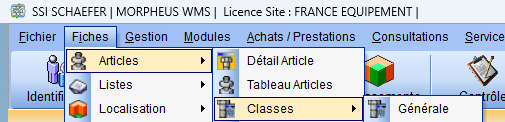
\includegraphics[width=0.9\linewidth]{images/mph_menu.png}
					\end{center}
					\caption{Teil des Menüs der bestehenden Morpheus-Anwendung}
					\floatfoot{Bildquelle : Screenshot}
					\label{fig:mph_menu}
				\end{figure}

\newpage

				\begin{figure}[ht!]
					\begin{center}
						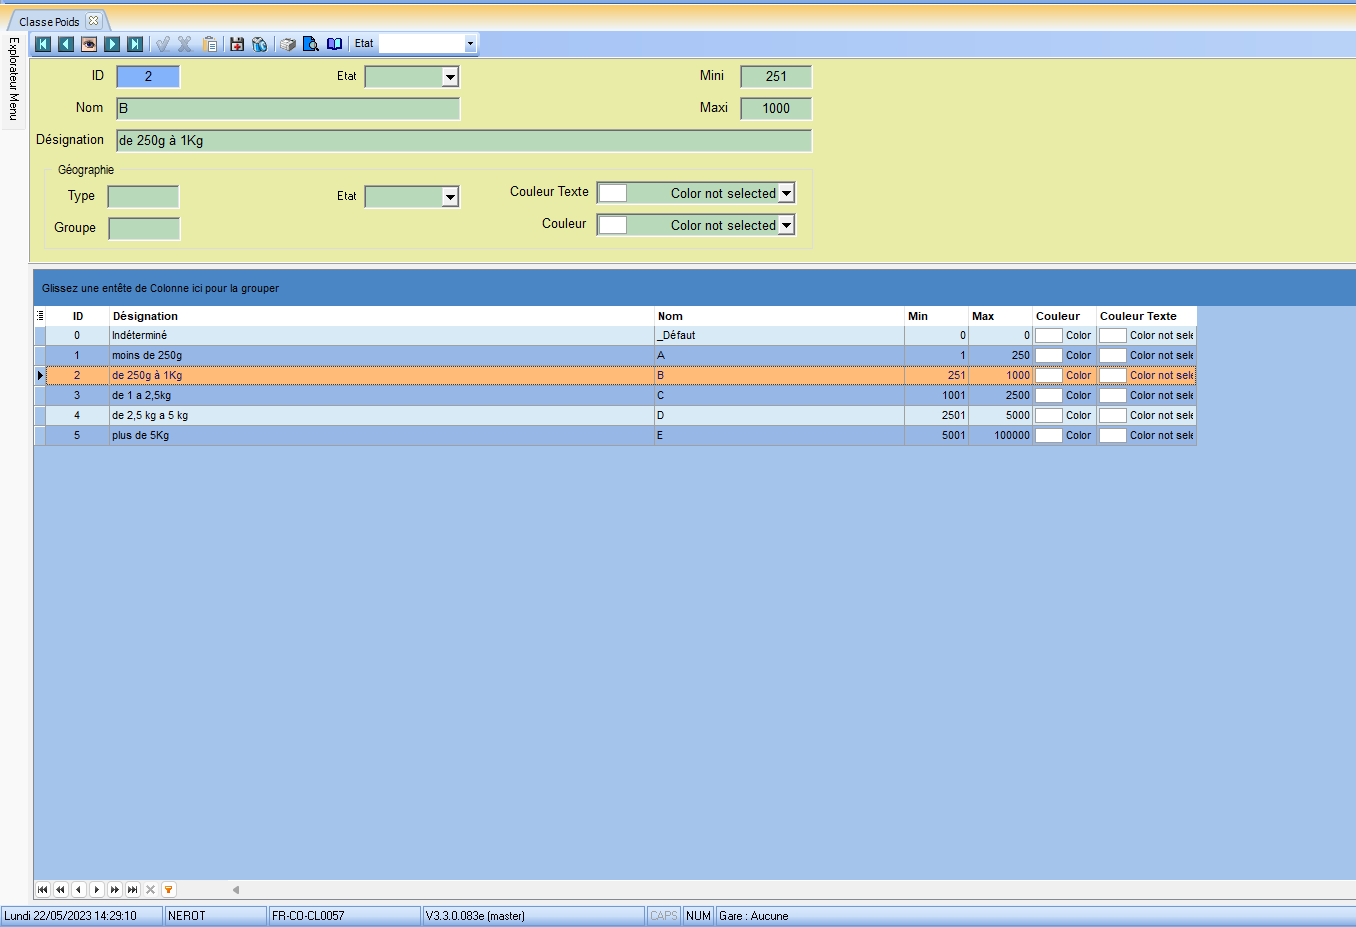
\includegraphics[width=\linewidth]{images/mph_window.png}
					\end{center}
					\caption{Beispiel eines vorhandenen Morpheus-Anwendungsfensters}
					\floatfoot{Bildquelle : Screenshot}
					\label{fig:mph_window}
				\end{figure}

				Obwohl der Morpheus-Client über viele Funktionen verfügt, ist er langsam in die Jahre gekommen. Somit verleiht das Webanwendungsentwicklungsprojekt ihm mit erneuerten grafischen Oberflächen auch ein zweites Leben. Darüber hinaus können Manager ihre Verwaltungsvorgänge direkt über ihren Browser ausführen und müssen den umfangreichen Client nicht mehr installieren.
				
		\newpage
		
		\part{Enjeux et importances}
			Au cours de mon stage au sein de SSI SCHÄFER, j'ai eu l'opportunité de travailler sur un projet d'une importance stratégique considérable. Ce projet n'était pas simplement une tâche parmi d'autres, mais il incarnait un défi clé que l'entreprise cherchait à relever pour atteindre ses objectifs à long terme. Dans cette section, je vais mettre en lumière les enjeux majeurs auxquels ce projet répondait et expliquer pourquoi sa réalisation revêtait une signification cruciale pour SSI SCHÄFER.\\

			Au-delà des aspects techniques, ce projet avait un impact direct sur la capacité de l'entreprise à prospérer dans un environnement concurrentiel en constante évolution. Il s'agissait d'une opportunité de consolider sa position sur le marché et de répondre aux attentes changeantes de ses clients. Tout au long de cette section, je vais détailler les aspects stratégiques et opérationnels qui ont rendu ce projet essentiel, ainsi que les résultats tangibles que j'ai pu obtenir grâce à mon travail acharné.\\

			En comprenant les enjeux et l'importance de ce projet, vous pourrez mieux apprécier la contribution significative que j'ai apportée à l'entreprise pendant mon stage, ainsi que la manière dont mes actions ont eu un impact direct sur ses objectifs globaux.
				
			\section{Enjeux du projet global}
				Chaque projet, qu'il soit grand ou petit, naît d'une nécessité, d'un défi ou d'un besoin spécifique. Mon expérience de stage au sein de SSI SCHÄFER m'a permis de plonger au c\oe ur d'un projet passionnant, dont la genèse repose sur des enjeux initiaux essentiels. Cette section est dédiée à l'exploration de ces enjeux, qui ont été le point de départ de cette aventure.\\

				Au cours de cette section, je vais détailler ces enjeux initiaux, identifier les contraintes qui se posaient, et montrer pourquoi il était impératif de mettre en place ce projet. Comprendre ces enjeux est la clé pour appréhender l'évolution du projet, les décisions prises en cours de route et les résultats obtenus. En saisissant les défis initiaux, vous serez en mesure de mesurer l'impact positif de mon travail dans la résolution de ces enjeux, et comment cela a contribué à l'entreprise.\\

					\subsection{Enjeux financiers}
						Le développement d'une \gls{app_web} Morpheus n'a pas pour premier enjeu un enjeu financier. En effet le projet a pour but de mener à une nouvelle communication sur le logiciel et offrir aux clients de nouvelles fonctionnalités. Néanmoins on peut imaginer qu'à plus long terme, la création d'une \gls{app_web} Morpheus peut avoir pour enjeu d'attirer de nouveaux clients.
	
					\subsection{Enjeux stratégiques}
						Le projet a pour enjeux stratégiques de permettre à l'entreprise de communiquer sur la suite de logiciels Morpheus et promouvoir de nouvelles fonctionnalités et un accès facilité à Morpheus auprès des clients.

					\subsection{Enjeux humains}
						Les enjeux humains du projet incluent la possibilité pour les clients d'accéder à Morpheus pour effectuer des opérations de gestion depuis leurs bureaux, sans nécessiter une présence dans l'entrepôt ni l'installation d'un \gls{client_lourd}, en utilisant simplement un navigateur web. Le projet vise également à réduire le temps que les techniciens passent à installer le nouveau client Morpheus. Puisqu'il suffirait simplement de déployer l'application sur un serveur web et non à installer un client sur chaque poste.
				
				\section{Objectifs globaux}
					Dans cette section, nous nous pencherons sur les objectifs globaux de notre projet, une étape fondamentale pour éclairer mon chemin vers la réalisation de mes aspirations. Ces objectifs constituent les piliers qui soutiendront mon initiative du début à la fin, et ils définissent la vision que je cherche à concrétiser. Nous parlerons ici des objectifs du projet global, nous reviendrons sur les objectifs du projet réalisé au cours du stage juste après dans la prochaine sous-section.
					
					Voici donc les objectifs globaux du projet :
					\begin{itemize}
						\bdot{Développer un client web morpheus (à partir du \gls{client_lourd} existant)}
						\bdot{Rendre morpheus plus accessible}
						\bdot{Créer un nouveau design ergonomique pour morpheus}
						\bdot{Faire une \gls{app_web} responsive accessible depuis n'importe quel terminal}%mettre définition terminal.. dans glossaire
					\end{itemize}
				
				\section{Enjeux du projet de stage}
					Le principal enjeu du projet de stage consistait à explorer diverses possibilités de développement pour le projet et à établir des fondations solides en vue de sa poursuite à long terme.
				
				\section{Objectifs du projet de stage}
					Voici une présentation sommaire des objectifs du projet de stage sur lesquels nous reviendrons par la suite.
					\begin{itemize}
						\bdot{Tester les outils de développement}
						\bdot{Créer une maquette}
						\bdot{Créer une première version de l'\gls{app_web}}
					\end{itemize}

				\section{Parties prenantes et intervenants}
					\noindent Voici les principales parties prenantes et intervenants qui ont pris part activement durant la réalisation de ce projet.

					\begin{itemize}
						\bdot{Monsieur Laurent GOURDON : directeur général France}
						\bdot{Monsieur Thierry NEROT : chef de projet et développeur du nouveau \gls{client_lourd} mopheus}
					\end{itemize}
				
				\section{Contraintes et limitations du projet de stage}
					Tout projet, qu'il soit de petite ou de grande envergure, est confronté à des contraintes et à des limitations qui peuvent influencer sa planification, son exécution et ses résultats. Dans cette section, nous allons explorer les défis et les restrictions spécifiques auxquels j'ai dû faire face tout au long de mon projet.\\

					La reconnaissance et la gestion des contraintes et des limitations sont essentielles pour une gestion de projet efficace. Ces facteurs peuvent être de nature diverse, qu'il s'agisse de contraintes budgétaires, de délais serrés, de ressources limitées, de contraintes techniques, ou d'autres obstacles potentiels. Dans cette partie, je vais détailler les contraintes et les limitations qui ont marqué mon projet et expliquer comment je les ai abordées.
					
					\subsection{Contraintes de délai}
						L'une des contraintes cruciales auxquelles j'ai été confronté pendant ce stage était la durée limitée qui m'a été accordée pour accomplir mes missions et atteindre les objectifs du projet. Le stage était fixé à une période de 27 semaines, ce qui représentait un défi en termes de planification et d'exécution.\\

						\subsubsection{Durée fixe du stage}
							Conformément aux exigences de l'établissement d'enseignement et de l'entreprise d'accueil, le stage était prévu pour une durée fixe de 27 semaines. Cette contrainte temporelle était immuable et ne pouvait pas être prolongée.

						\subsubsection{Complexité du projet}
							Le projet sur lequel j'ai travaillé était d'une certaine complexité, avec des objectifs ambitieux à atteindre. Cette complexité a rendu la gestion du temps d'autant plus cruciale.

						\subsubsection{Apprentissage et conception initiale}
							Une période initiale était nécessaire pour me familiariser avec l'entreprise, ses processus, et les spécificités du projet. Cela signifiait que je disposais en réalité de moins de temps pour la phase active de développement.

						\subsubsection{Solutions}
							Face à cette contrainte de durée, j'ai adopté une approche stratégique pour maximiser mon efficacité.

							\paragraph{Planification avancée\\}
								Dès le début du stage, avec Monsieur NEROT, chef du projet, nous avons élaboré un plan détaillé, en identifiant les tâches essentielles à accomplir et en les répartissant sur la période disponible.

							\paragraph{Priorisation des tâches\\}
								Nous avons établi des priorités claires en fonction des objectifs du projet et de leur importance stratégique, afin de nous concentrer sur les éléments les plus critiques en premier.\\

				\vspace{\baselineskip}
				Malgré la contrainte de durée du stage, j'ai réussi à atteindre mes objectifs en me concentrant sur l'efficacité, la planification minutieuse et la gestion rigoureuse du temps. Cette expérience m'a permis d'acquérir des compétences précieuses en gestion du temps et en prise de décision stratégique.
				\newpage
					\subsection{Limitations en ressources humaines}
						\subsubsection{Effectif limité et surchage de travail}
							Tout d'abord, il est important de rappeler, que j'ai principalement travailler seul sur le projet de création de l'\gls{app_web} Morpheus. Paradoxalement, une des principales limitations auxquelles j'ai été confronté tout au long de ce stage était liée aux ressources humaines. En effet l'équipe de développeurs est composée de quatres personnes, en plus de moi en tant que stagiaire, qui ont toutes déjà un emploi du temps très chargé. Il est dont apparu certaines problématiques lorsque j'avais besoin de l'aide ou de la participation de mes collègues au projet. Il me revient en tête un exemple assez significatif. Alors que j'avancais sur la partie \gls{frontend} de l'application, Monsieur NEROT devait développer l'\acrshort{api} qui me permettrait de faire des requêtes à la base de données. Cependant étant très surchargé il n'a pas pu me fournir l'\acrshort{api} dans les temps souhaités.
						
						\subsubsection{Solutions}
								Pour pallier à cette limitation en ressources humaines, nous avons mis en place des méthodes de communication efficaces afin de ne pas perdre de temps lorsque nous avions à échanger à propos du projet. De plus j'ai pris la responsabilité de développer moi-même une \acrshort{api} afin de pouvoir tester la connexion à la base de données.

					\subsection{Conclusion}
							Au cours de ce projet, j'ai été confronté à un ensemble varié de contraintes et de limitations, chacune apportant son propre défi. Cependant, au lieu de voir ces contraintes comme des obstacles insurmontables, je les ai abordées comme des opportunités d'apprentissage et de croissance.\\

							La gestion des contraintes, des délais serrés, des ressources humaines limitées, et d'autres défis m'a permis de développer des compétences essentielles en gestion de projet, en résolution de problèmes, et en collaboration. Ces expériences m'ont montré que, même lorsque les ressources sont limitées, une planification minutieuse, une communication efficace, et une approche stratégique peuvent conduire à des résultats réussis.\\

							En fin de compte, la gestion des contraintes et des limitations a été une expérience formatrice qui a renforcé ma compréhension de la réalisation de projets dans des conditions du monde réel. Je suis fier des résultats que j'ai obtenus malgré ces défis, et je suis convaincu que ces compétences acquises me seront bénéfiques dans mes futures entreprises professionnelles.

			\section{Synthèse des enjeux et de l'importance}
				Pendant mon stage chez SSI SCHÄFER, j'ai travaillé sur un projet stratégique de grande importance, allant au-delà d'une simple tâche. Ce projet visait à relever des défis clés pour l'entreprise à long terme. Dans cette synthèse, je vais mettre en lumière les enjeux majeurs du projet, expliquer son importance pour SSI SCHÄFER, détailler les objectifs globaux, évoquer les contraintes rencontrées, et mettre en avant mon approche pour les surmonter.\\

				Le projet avait un impact direct sur la compétitivité de l'entreprise dans un marché en constante évolution. Il visait à consolider sa position et à répondre aux attentes changeantes des clients. Le projet répondait à des enjeux financiers, en améliorant la communication sur le logiciel Morpheus et en offrant de nouvelles fonctionnalités. Il avait également des enjeux stratégiques, favorisant la promotion de Morpheus et son accessibilité. Les enjeux humains permettront aux clients de gérer Morpheus depuis leurs bureaux via un navigateur web.\\

				Les objectifs globaux du projet comprenaient le développement d'un client web Morpheus, le rendant plus accessible et ergonomique, ainsi que la création d'une \gls{app_web} responsive.\\

				Le principal enjeu du projet de stage était d'explorer les possibilités de développement et de poser des bases solides pour l'avenir.\\

				Les objectifs du projet de stage incluaient le test des outils de développement, la création d'une maquette et d'une première version de l'\gls{app_web}.\\

				Les parties prenantes comprenaient le directeur général de SSI SCHÄFER France ainsi que le chef de projet et développeur du nouveau client Morpheus.\\

				Le projet était soumis à des contraintes de délai, avec une période de stage fixe de 27 semaines. La complexité du projet et la nécessité d'une phase d'apprentissage initiale ont renforcé cette contrainte. Malgré cela, une planification avancée et une priorisation des tâches ont permis d'atteindre les objectifs.\\

				Les limitations en ressources humaines, avec une équipe restreinte, ont également influencé le projet, mais malgré cela, des compétences essentielles en gestion de projet ont été développées.\\

				En conclusion, ce projet a été une opportunité d'apprentissage et de croissance malgré les contraintes et les limitations. La gestion efficace de ces défis a renforcé mes compétences et me servira dans ma future carrière professionnelle.

		\newpage

		\part{Méthodologie et outils}\label{section:methodologie}
			La réussite d'un projet repose souvent sur une méthodologie solide et l'utilisation adéquate d'outils appropriés. Au cours de mon stage au sein de SSI SCHÄFER, j'ai eu l'opportunité de travailler sur un projet stimulant qui nécessitait une approche réfléchie et une utilisation judicieuse des ressources technologiques. Dans cette section, je vais vous présenter la méthodologie que nous avons adoptée pour mener à bien ce projet ainsi que les outils technologiques qui ont été essentiels à sa réalisation.\\

			La méthodologie que nous avons choisie pour aborder ce projet a joué un rôle déterminant dans ma capacité à atteindre mes objectifs de manière efficace et efficiente. De plus, les outils que j'ai sélectionnés ont facilité la gestion, la collaboration et la mise en œuvre de ce projet complexe. En comprenant la méthodologie et les outils que j'ai utilisés, vous aurez une vision plus précise de la manière dont j'ai planifié et exécuté ce projet avec succès.

			\section{Méthodologie adoptée}
				La réalisation de tout projet réussi repose sur une méthodologie solide et des approches bien définies. Dans cette section, nous allons plonger dans les détails de la méthodologie que j'ai adoptée pour concevoir, développer et mettre en œuvre mon projet.\\

				La méthodologie adoptée a été un élément clé de mon succès, en m'aidant à maintenir la structure, la cohérence et la qualité tout au long du processus. Cette section jettera les bases pour la suite de la présentation, où nous explorerons les résultats obtenus grâce à l'application de cette méthodologie.
				
				\newpage
				\subsection[Choix de la méthodologie : méthode en V]{\printSectionFootnote{subsection:modele_v}{wikipedia:modele_v}}\label{subsection:modele_v}%mettre en annexe une présentation plus détaillé de la méthode en v.. + lien wikipedia..
					Le modèle en V est un cadre d'organisation des activités de développement d'un produit. Il se caractérise par deux flux d'activités : l'un descendant qui décompose le produit jusqu'à sa réalisation, et l'autre ascendant qui assemble le produit tout en vérifiant sa qualité. Ce modèle découle de l'approche séquentielle et linéaire du modèle en cascade, mais il l'enrichit en intégrant des activités d'intégration système à partir de composants plus élémentaires. De plus, il associe chaque phase de production à sa phase de validation correspondante, créant ainsi une structure en forme de V.\\

					Dérivé de l'ingénierie système, le modèle en V est souvent perçu comme un cycle de projet, bien que l'ingénierie système et la gestion de projet soient complémentaires. L'ingénierie système se concentre sur le développement du produit, tandis que la gestion de projet vise à atteindre les avantages escomptés par le client ou l'utilisateur. Il est donc important de noter que le modèle en V ne constitue pas en lui-même un cycle de projet.\\

					Comme nous le verrons tout au long de cette section, même si le projet n'a pas suivi parfaitement les étapes d'une méthologie en V, on peut y retrouver beaucoup de similitudes.

				\newpage
				\subsection{Étapes de la méthodologie}
					\begin{figure}[h!]
						\begin{center}
							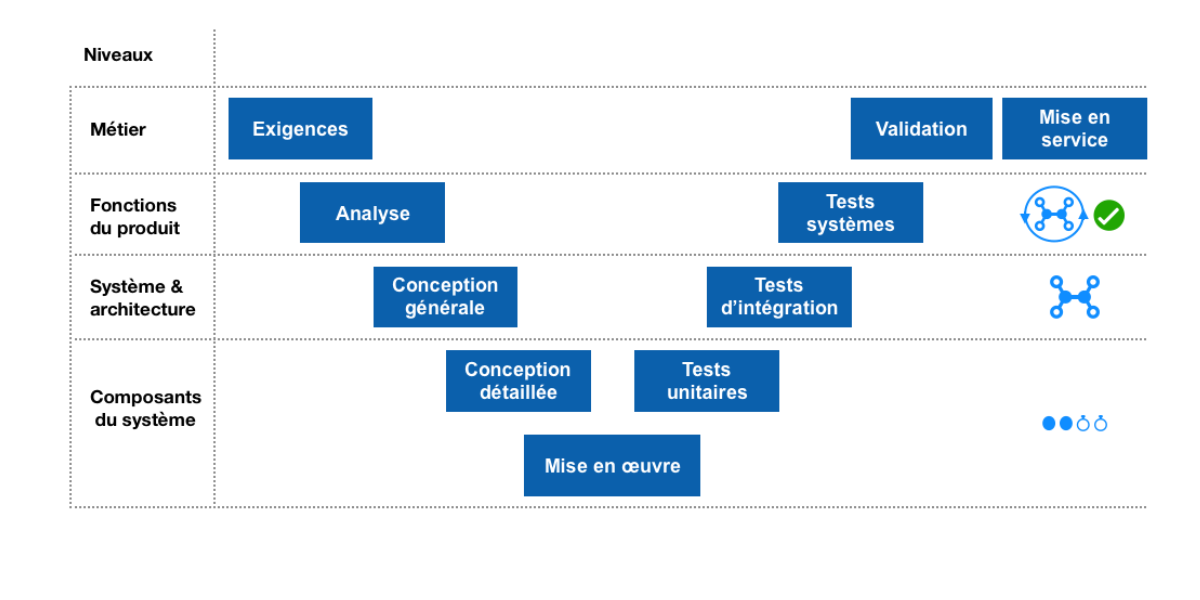
\includegraphics[width=\linewidth]{images/cycle_v_etapes.png}
						\end{center}
						\caption{Étapes de la méthodologie en V}
						\floatfoot{Source de l'image : \url{https://upload.wikimedia.org/wikipedia/commons/9/9d/Cycle_en_V_g\%C3\%A9n\%C3\%A9ral.png?uselang=fr}}
						\label{fig:cycle_v_etapes}
					\end{figure}			

			\section{Planification et gestion de projet}
				Au cœur de tout projet réussi réside une planification minutieuse et une gestion efficace. Dans cette section, nous allons plonger dans les détails de la manière dont mon projet a été structuré, planifié et géré pour atteindre ses objectifs.\\

				La planification et la gestion de projet sont des éléments cruciaux qui guident chaque étape de notre travail. Elles nous permettent d'établir des fondations solides, de définir des priorités, de gérer les ressources et de maintenir le cap tout au long du parcours. Dans cette partie, nous allons explorer les principes et les pratiques que j'ai mis en place pour assurer le succès de mon projet.\\

				Chaque aspect de la planification et de la gestion de projet a contribué à ma capacité à atteindre mes objectifs, à respecter les délais et à maintenir la qualité de mon travail. En comprenant ces processus, vous aurez une vue d'ensemble claire de la façon dont mon projet a été dirigé du début à la fin.

				\subsection{Planification}
					Phases initiales du projet :
					\begin{itemize}
						\bdot{Installation et configuration des outils}
						\bdot{Expérimentation des outils}
						\bdot{Rédaction détaillée des besoins}
						\bdot{Développement du nouveau client \gls{html}5}
						\bdot{Test et recettage du nouveau client}
						\bdot{Livraison}
					\end{itemize}
				
				\subsection{Diagramme de GANTT}
					\noindent Voici le diagramme de GANTT de mon projet :
					\begin{figure}[ht!]
						\begin{center}
							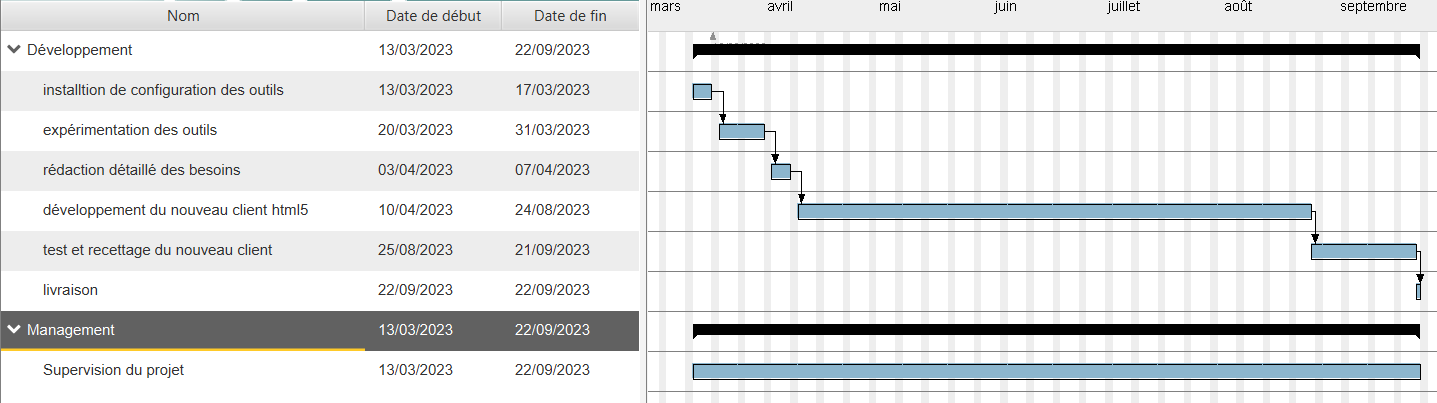
\includegraphics[width=\linewidth]{images/gantt_initial.png}
						\end{center}
						\caption{Diagramme de GANTT initial du projet réalise au cours du cours}
						\floatfoot{Source de l'image : capture d'écran}
						\label{fig:gantt_initial}
					\end{figure}	
					
					Malheureusement nous n'avons pas eu le temps de faire le recettage, néanmoins des tests ont été faits et j'ai rendu mon travail à mon entreprise d'accueil.

				\subsection{Budgétisation}
					Le budget du projet est composé des éléments suivants :
					\begin{itemize}
						\bdot{Investissement des outils \gls{tmssoftware} : 1800€}
						\bdot{25 semaines * 5 jours * 750€ : budget temps passé au développement}
						\bdot{7 semaines * 1 jour * 950€ : budget temps passé au management}
					\end{itemize}
						
				\section[Confluence : outil de gestion de la documentation]{\printSectionFootnote{subsection:confluence}{wikipedia:confluence}}\label{subsection:confluence}
					Confluence est un logiciel de wiki, utilisé comme logiciel de travail collaboratif. Dans le cadre du projet de développement de l'\gls{app_web} morpheus, confluence m'a permis de documenter le projet et ainsi de permettre une reprise du projet simplifiée par un tiers.\\

					\begin{figure}[h!]
						\begin{center}
							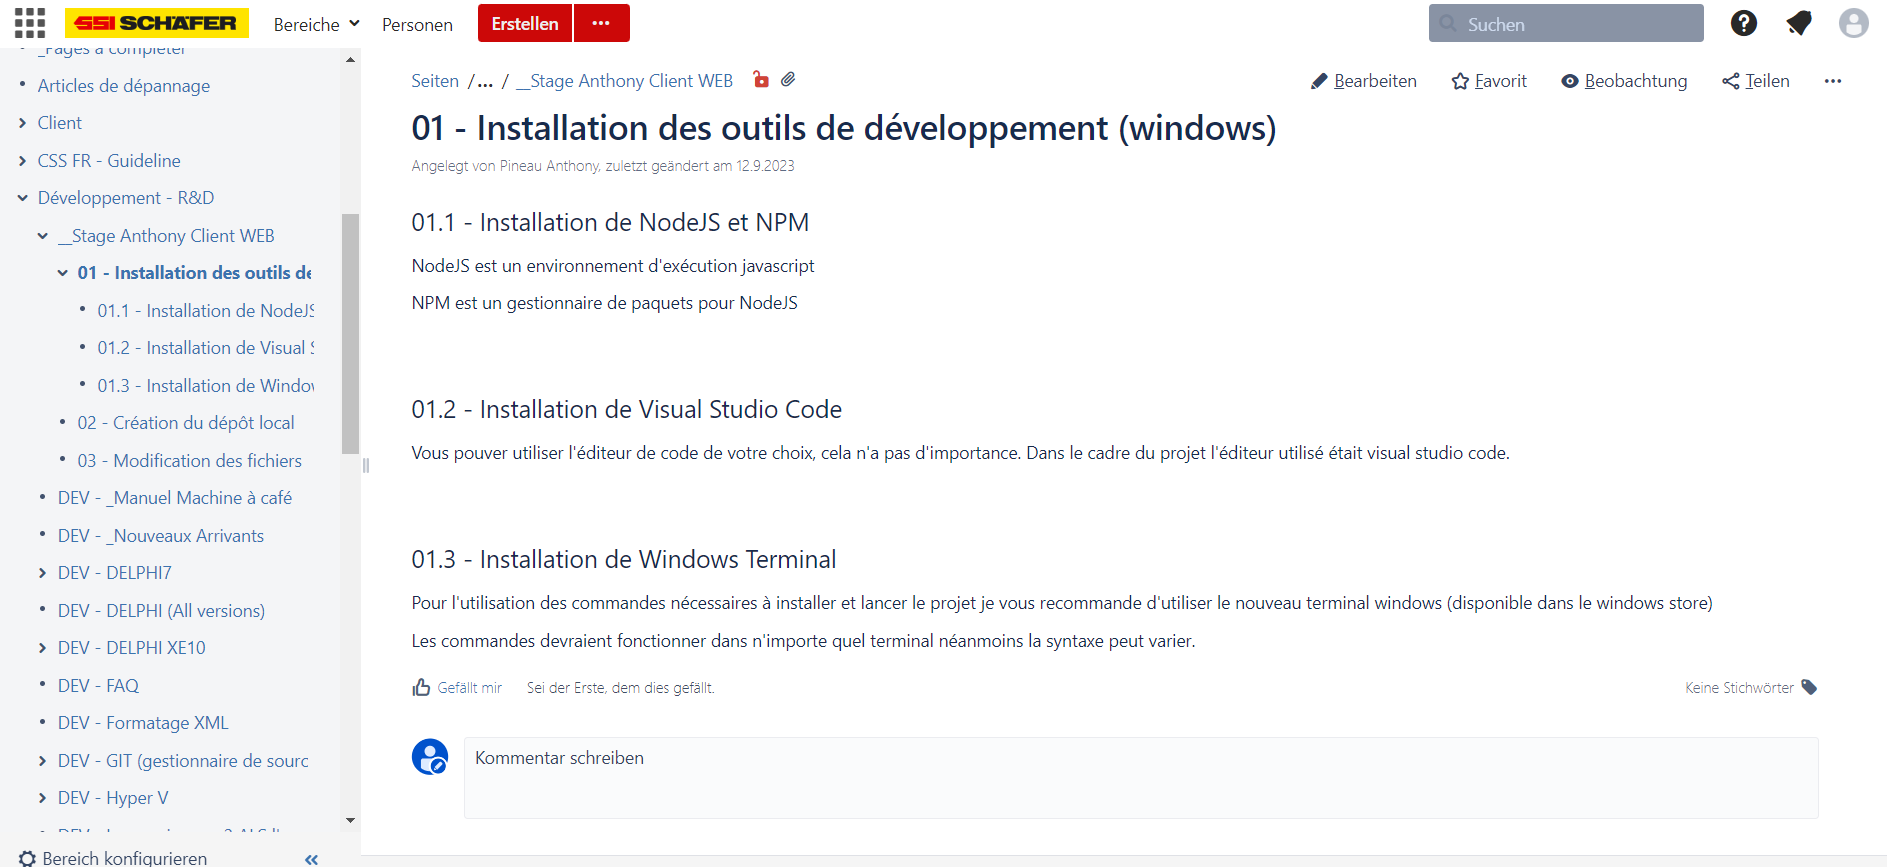
\includegraphics[width=\linewidth]{images/confluence_tools.png}
						\end{center}
						\caption{Extrait de la documentation émise sur confluence}
						\floatfoot{Source de l'image : capture d'écran}
						\label{fig:confluence_tools}
					\end{figure}	
					
					\begin{figure}[h!]
						\begin{center}
							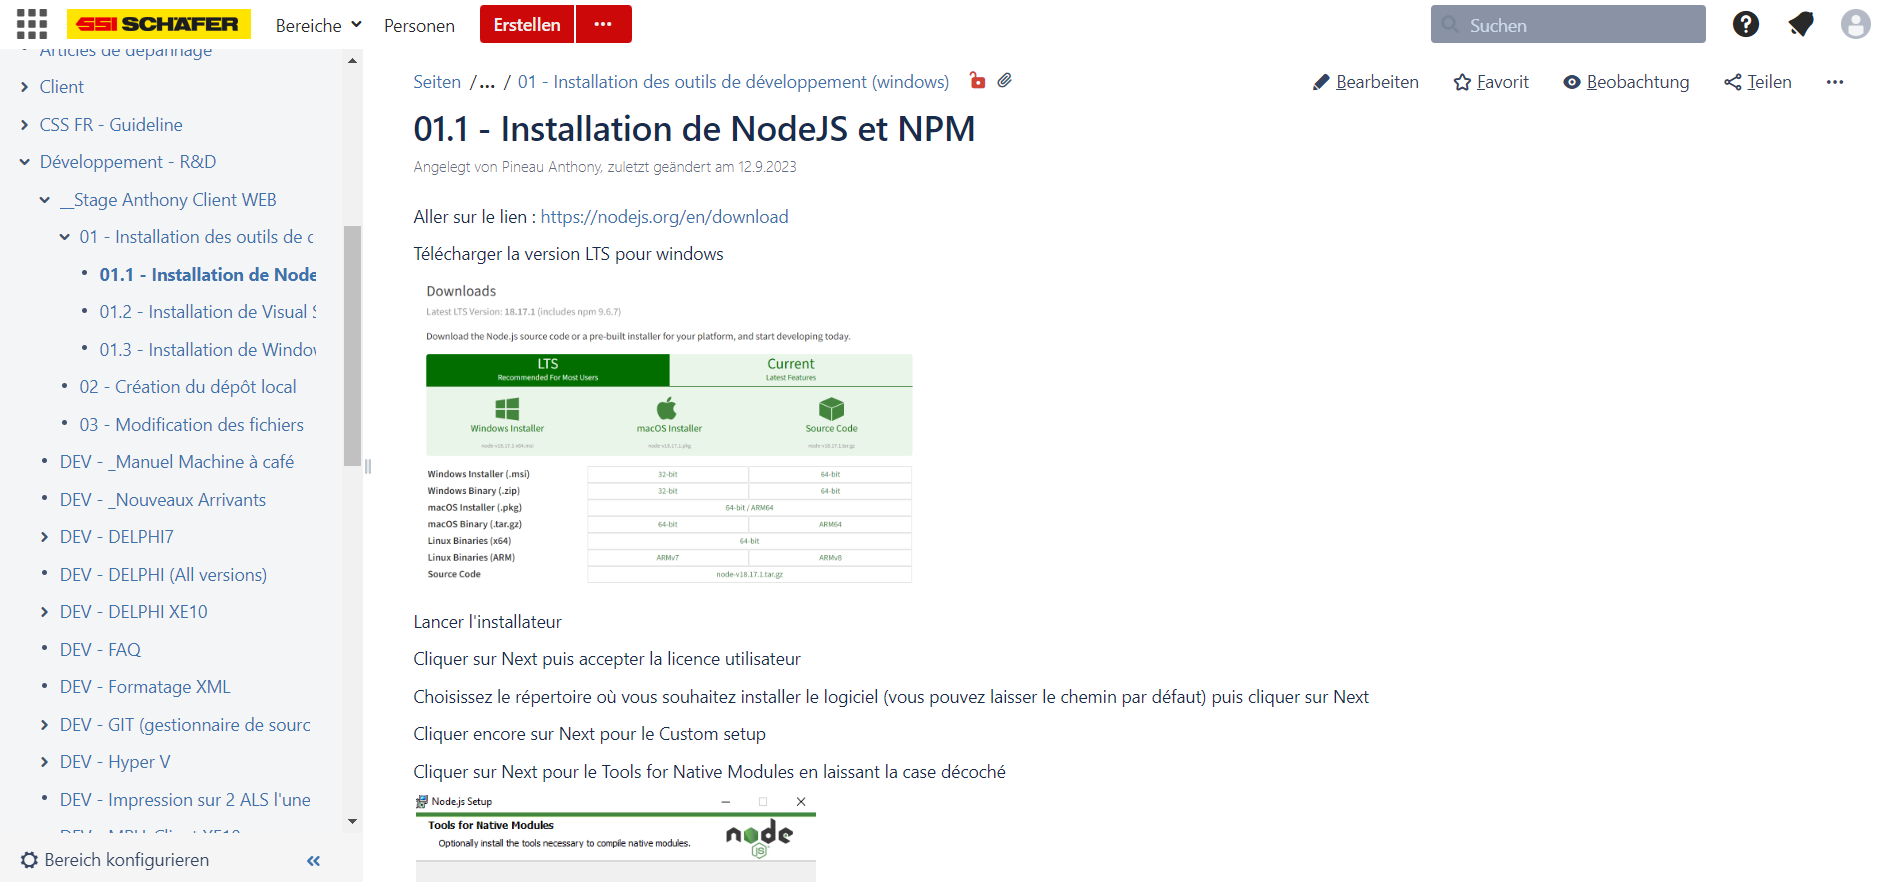
\includegraphics[width=\linewidth]{images/confluence_nodejs.png}
						\end{center}
						\caption{Extrait de la documentation émise sur confluence}
						\floatfoot{Source de l'image : capture d'écran}
						\label{fig:confluence_nodejs}
					\end{figure}	

					%\noindent Vous retrouverez en Annexe la documentation détaillée émise au cours du projet.

	%Mettre screenshot..
	%+pdf en annexe (export de confluence)
	
			\section{Collaboration et communication}
				La réussite d'un projet ne repose pas seulement sur la qualité de la planification et de l'exécution, mais également sur la manière dont les membres de l'équipe collaborent et communiquent. Dans cette section, nous allons explorer comment la collaboration efficace et la communication transparente ont été des piliers de ma réussite tout au long de ce projet.\\

				Dans cette partie, nous allons détailler les méthodes, les outils et les pratiques que nous avons utilisés pour favoriser la collaboration au sein de l'équipe. Nous examinerons également comment la communication a été structurée pour assurer la circulation fluide de l'information.
				\newpage
				\subsection[Teams : outil de messagerie instantanée]{\printSectionFootnote{subsubsection:teams}{wikipedia:teams}}\label{subsubsection:teams}
					Microsoft Teams est une plateforme de collaboration et de communication professionnelle développée par Microsoft. Elle permet aux équipes de travail de collaborer en temps réel, que ce soit au sein d'une même entreprise ou entre différentes organisations. Microsoft Teams offre une gamme de fonctionnalités, notamment la messagerie instantanée, la vidéoconférence, le partage de fichiers, la gestion de tâches, l'intégration d'applications tierces, et bien plus encore.\\

					Teams s'avère extrêmement pratique pour faciliter la communication avec les collègues, particulièrement lorsqu'ils travaillent à distance. De plus, il sert de manière très pratique pour la tenue de réunions en ligne. Pendant mon stage, j'ai principalement eu recours à Teams pour exploiter ces deux fonctionnalités.
					
				\subsection[Outlook : outil de messagerie]{\printSectionFootnote{subsubsection:outlook}{wikipedia:outlook}}\label{subsubsection:outlook}
					Outlook est un client de messagerie électronique qui permet aux utilisateurs de gérer leurs e-mails, leurs calendriers, leurs tâches, leurs contacts et leurs notes en un seul endroit. Il offre un ensemble de fonctionnalités qui facilitent la communication, la planification et l'organisation de tâches professionnelles et personnelles. Les principales caractéristiques d'Outlook comprennent la réception et l'envoi d'e-mails, la gestion des calendriers pour planifier des rendez-vous et des réunions, la création de tâches pour suivre les activités à accomplir, la gestion des contacts pour organiser les informations de contact, et la possibilité de prendre des notes.\\

					Pendant mon stage, j'ai principalement utilisé Outlook pour l'envoi de courriels à mes collègues et à Monsieur Hamrioui. Mais j'ai aussi profité de ses autres fonctionnalités pour planifier diverses tâches, rendez-vous et réunions grâce au calendrier intégré dans l'application.

				\subsection{"Point dev" : réunion hebdomadaire}
					Toutes les semaines, le vendredi à 14H, nous effectuions une réunion, appelée "Point dev", qui réunissait tous les développeurs de l'entreprise. Durant cette réunion, chachun indiquait ce qu'il avait fait pendant la semaine écoulée et pouvait parler des problèmes rencontrés. Cela permettait aussi de trouver des solutions aux problèmes évoqués.

				\subsection{Réunions ponctuelles}
					Parfois nous faisions des réunions avec Monsieur GOURDON et Monsieur NEROT afin de parler de l'avancement du projet et vérifier qu'il avancait toujours dans la bonne direction.
				
				\subsection{Communication avec les collègues}
					Bien que j'étais principalement seul à travailler sur le projet, je pouvais, si besoin, discuter avec mes collègues des problèmes rencontrés et chercher ensemble une solution. La communication avec eux a toujours été facile et fluide et a partcipé à la bonne réussite du projet.
			
			\section{Outils technologiques}				
				Les avancées technologiques ont transformé la manière dont nous concevons, développons et mettons en œuvre des projets. Dans cette section, nous allons explorer les outils technologiques que j'ai exploités pour donner vie à mon projet et atteindre mes objectifs.\\

				Dans cette partie, je vais présenter les outils technologiques spécifiques que j'ai utilisés, en expliquant pourquoi je les ai choisis. Nous allons détailler comment ces outils ont contribué à la réalisation de mes objectifs et comment ils ont amélioré mon efficacité tout au long du projet.
				\newpage
				\subsection[\gls{delphi}]{\printSectionFootnoteS{subsection:delphi}{methodologie:outils_technologiques:delphi, methodologie:outils_technologiques:delphi:tms_software, methodologie:outils_technologiques:delphi:tms_web}}\label{subsection:delphi}
					\gls{delphi} est à la fois un \gls{langage_programmation} \gls{poo} et un \gls{EDI} (\acrshort{edi}) pour ce langage. \gls{delphi} est un \acrshort{edi} propriétaire fonctionnant sous Windows créé en 1995 par Borland. \gls{delphi} embarque une version \glspl{poo} du langage Pascal : le Pascal Objet, renommé \Gls{langage_programmation} \gls{delphi} au fil des modifications apportées par Borland.\\

					Dans le cadre de mon projet, \gls{delphi} a été le premier \gls{langage_programmation} envisagé pour réaliser l'\gls{app_web} Morpheus. Avec l'utilisation du \gls{framework} \gls{tmsweb} de \gls{tmssoftware}, j'ai pu créer la première version de l'\gls{app_web}
					
					\subsubsection{\gls{tmssoftware} et \gls{tmsweb}}\label{subsubsection:tms}
						\paragraph{\gls{tmssoftware}\\}
							La société \gls{tmssoftware} est une entreprise de développement de logiciels spécialisée dans :
							\begin{itemize}
								\bdot{Le développement de composants VCL, FMX, LCL, FNC, ASP.NET, .NET, IntraWeb}
								\bdot{Des projets de développement pour Windows, le Web, Android, iOS, macOS, Linux, et Node.js}
								\bdot{La formation, le conseil et le développement de projets personnalisés.}
							\end{itemize}
					
						\paragraph{\gls{tmsweb}}
							\gls{tmsweb} est un \gls{framework} permettant de créer des \glspl{app_web} en \gls{delphi}.
					
					D'abord envisagé parce que déjà utilisé par l'entreprise, cet outil technologique m'a permis de me rendre compte qu'il n'était pas le plus adapté pour le projet et a participé au choix d'une technologie plus adapté.
				\newpage
				\subsection[\gls{html}]{\printSectionFootnote{subsection:html}{wikipedia:html}}\label{subsection:html}
					Le HyperText Markup Language, couramment abrégé en \gls{html}, représente le langage de balisage conçu pour la création de pages web. Ce langage permet la rédaction d'\gls{hypertexte}, la structuration sémantique des pages web, la mise en forme de contenu, la création de formulaires interactifs et l'intégration de ressources multimédias telles que des images, des vidéos et des scripts informatiques. L'\gls{html} offre également la possibilité de créer des documents compatibles avec une grande variété de dispositifs, en respectant les normes d'accessibilité du web. \gls{html} est donc le langage que j'ai utilisé pour la création de toutes mes pages web.
				
				\subsection[\gls{css}]{\printSectionFootnoteS{subsection:css}{wikipedia:css, wikipedia:sass}}\label{subsection:css}
					Les feuilles de style en cascade, souvent abrégées en \gls{css} à partir de l'anglais Cascading Style Sheets, représentent un langage informatique utilisé pour définir la mise en forme des documents \gls{html} et \gls{XML}.\\
					
					\subsubsection{Sass}
						Sass (Syntactically awesome stylesheets) est un langage de script préprocesseur\footnote{Retrouver en annexe plus d'informations sur ce qu'est un langage de script préprocesseur} qui est compilé ou interprété en \gls{css} (Cascading Style Sheets).\\
				
						\gls{css} et Sass ont été les prinipaux outils que j'ai utilisés pour mettre en forme mes pages web.

				\subsection[\gls{javascript}]{\printSectionFootnoteS{subsection:javascript}{wikipedia:javascript, wikipedia:typescript, wikipedia:react, devexpress}}\label{subsection:javascript}
					\gls{javascript} est un \gls{langage_programmation} de scripts principalement employé dans les pages web interactives et à ce titre est une partie essentielle des \glspl{app_web}. Avec les langages \gls{html} et \gls{css}, \gls{javascript} est au cœur des langages utilisés par les développeurs web. Une grande majorité des sites web l'utilisent, et la majorité des navigateurs web disposent d'un moteur \gls{javascript} pour l'interpréter.

					\subsubsection{Typescript}
						TypeScript représente un \gls{langage_programmation} \gls{opensource} créé par Microsoft dans l'optique d'améliorer et de renforcer la qualité de la production de code \gls{javascript}. Il s'érige comme un sur-ensemble syntaxique rigoureux de \gls{javascript}, ce qui signifie que tout code \gls{javascript} valide est également compatible avec TypeScript. Le code TypeScript est transformé en \gls{javascript} via une opération de transcompilation, permettant ainsi son interprétation par n'importe quel navigateur web ou moteur \gls{javascript}.

					\subsubsection{\gls{react}}\label{subsubsection:react}
						\gls{react} (également connu sous le nom de React.js ou ReactJS) est une \gls{bibliotheque_logicielle} \gls{javascript} \gls{opensource} développée par Facebook (aujourd'hui Meta) à partir de 2013. L'objectif principal de cette \gls{bibliotheque_logicielle} est de simplifier la création d'\glspl{app_web} monopages en permettant la création de composants dépendants de l'état, qui génèrent une page (ou une portion de page) \gls{html} à chaque modification de cet état.\\

						\gls{react} se concentre exclusivement sur la gestion de l'interface utilisateur de l'application, considérée comme la vue dans le modèle \acrshort{mvc} (\gls{MVC}). Par conséquent, elle peut être utilisée en combinaison avec d'autres \gls{bibliotheque_logicielle}s ou \glspl{framework} \acrshort{mvc} tels qu'AngularJS. Ce qui distingue cette \gls{bibliotheque_logicielle} de ses concurrentes, c'est sa flexibilité et ses performances. Elle travaille avec un \acrshort{dom} virtuel et met à jour le rendu dans le navigateur uniquement lorsque cela est nécessaire, ce qui contribue à améliorer les performances de l'application.
					\newpage
					\subsubsection{\gls{devextreme} par \gls{devexpress}}\label{subsubsection:devextreme}
						\paragraph{DexExpress\\}
							Developer Express Inc. est une entreprise de développement de logiciels. Au départ, \gls{devexpress} produisait des contrôles d'interface utilisateur pour Borland \gls{delphi}/C++Builder et des contrôles ActiveX pour Microsoft Visual Studio. À l'heure actuelle, \gls{devexpress} propose des produits destinés aux développeurs qui utilisent \gls{delphi}/C++Builder, Visual Studio, ainsi que les technologies \gls{html}5/\gls{javascript}.

						\paragraph{\gls{devextreme}\\}
							De Angular et \gls{react} à Vue, \gls{devextreme} comprend une collection complète de composants d'interface utilisateur haute performance et réactifs pour une utilisation dans des \glspl{app_web} traditionnelles et des applications mobiles de nouvelle génération.
				
						Tous ces outils font partis des langages de programmation/\gls{framework} que j'ai utilisé pour développer l'\gls{app_web} Morpehus.

				\subsection[Git]{\printSectionFootnote{subsubsection:git}{wikipedia:git}}\label{subsubsection:git}
					Git est un \gls{vcs} décentralisé. Dans le projet, il m'a principalement servi à faire une sauvegarde régulière du code produit. Par ailleurs dans un projet où plusieurs développeurs travaillent en ensemble il est possible de créer différentes branches du projet, où chacun travaille sur sa partie, puis de fusionner les résultats obtenus.%en annexe expliquer logiciel de gestion de versions décentralisé..

				\subsection[Insomnia]{\printSectionFootnote{subsubsection:insomnia}{insomnia}}\label{subsubsection:insomnia}
					Insomnia, est une plateforme \gls{opensource} de Kong Inc. (en) pour tester des \acrshort{api}. Cet outil m'a permis de tester des requêtes sur l'\acrshort{api} que nous avons créé sans avoir besoin de développer quoi que ce soit.
				\newpage
				\subsection[Microsoft SQL Server \& Microsoft SQL Server Management Studio]{\printSectionFootnoteS{subsubsection:mssql}{wikipedia:mssql, wikipedia:mssqlstudio}}\label{subsubsection:mssql}
					\subsubsection{Microsoft SQL Server}
						Microsoft SQL Server est un \gls{SGBD} (\acrshort{sgbd}) en langage SQL incorporant entre autres un \acrshort{sgbd}R (\acrshort{sgbd} "relationnel").

					\subsubsection{Microsoft SQL Server Management Studio}
						Microsoft SQL Server Management Studio (SSMS) est une application logicielle développée par Microsoft qui est utilisée pour configurer, gérer et administrer tous les composants au sein de Microsoft SQL Server.

					Ces outils technologiques sont les outils utilisés par l'entreprise pour la gestion de la base de données de Morpheus. Ainsi ils ont donc été la base pour moi de la base de données que j'ai utilisée au cours du projet.

				\subsection[Visual Studio Code]{\printSectionFootnote{subsubsection:vscode}{wikipedia:vscode}}\label{subsubsection:vscode}
					Visual Studio Code est un éditeur de code extensible développé par Microsoft pour Windows, Linux et macOS. Les fonctionnalités incluent la prise en charge du débogage, la mise en évidence de la syntaxe, la complétion intelligente du code (IntelliSense.), les snippets, la refactorisation du code et Git intégré. Les utilisateurs peuvent modifier le thème, les raccourcis clavier, les préférences et installer des extensions qui ajoutent des fonctionnalités supplémentaires.\\

					Visual Studio Code est l'éditeur de code que j'utilise de nombreuses années, je sais donc assez bien comment l'utiliser. Il a donc été évident pour moi de l'utiliser dans ce projet afin d'être le plus productif possible et de ne pas perdre de temps à prendre en main un nouvel éditeur de code.
				
				\subsection[Modelio]{\printSectionFootnote{subsubsection:modelio}{wikipedia:modelio}}\label{subsubsection:modelio}
					Modelio est un outil de modélisation \acrshort{uml}. Il m'a notamment servi à créer le diagramme de classe des nouvelles tables de la base de données.
				
				\subsection[Latex]{\printSectionFootnote{subsubsection:latex}{wikipedia:latex}}\label{subsubsection:latex}
					LaTeX est un langage et un système de composition de documents. Il s'agit d'une collection de macrocommandes destinées à faciliter l'utilisation du « processeur de texte » TeX de Donald Knuth. J'ai notamment utilisé Latex pour la rédaction de ce mémoire ainsi que les rapports d'avancements durant tout le stage.			
		
		\newpage

		\part{Project progress (Déroulement du projet)\footnote{Retrouver la traduction de la partie Déroulement du projet en Annexe \ref{appendix:projet_translation} \nameref{appendix:projet_translation}}}
		The success of a project depends on its objective and tools, but also on how it is planned, executed and managed throughout its life cycle. During my internship at SSI SCHAEFER, I had the opportunity to participate in a large-scale project that required careful planning and rigorous execution. In this section, I will immerse you in the complete progress of this project, describing the different steps that I followed.

			\section{Objectives et initial planning}
				Clarity of objectives and methodical planning are the foundations of any successful project. In this section, we'll explore the goals I set at the start of my project and the initial planning that guided my actions.\\

				The process of defining objectives is a fundamental step in carrying out any project. In this part, we will detail these objectives, explain why they were chosen, and how they were aligned with the issues and needs that we identified previously.\\

				Initial planning is just as essential. It allows us to define the trajectory of the project, identify key stages, necessary resources, and set realistic deadlines. In this section, I will present the initial plan that I had in place.\\

				By understanding these elements, you will have a clear overview of how my project was designed and structured to achieve specific objectives, while taking into account the constraints and realities of the environnment. This part will lay the foundations for the rest of the dissertation, where I will detail the implementation and results in relation to these initial objectives.
				\newpage
				\subsection{Detailled objectives}
				\noindent The initial objectives of the project were:
	
					\begin{itemize}
						\bdot{Develop a morpheus client in full \gls{html} 5 and responsive for some windows of the existing Mopheus client}
						\bdot{Experiment the development tools of \gls{tmsweb}}
						\bdot{Make a UI mockup}
							\begin{itemize}
								\bdotoutlined{Main window}
									\begin{itemize}
										\bsquare{Menu}
											\begin{itemize}
												\bsquareoutlined{Icons}
												\bsquareoutlined{Style (as windows' style : colors)}
												\bsquareoutlined{X configurable levels and sub levels}
													\begin{itemize}
														\bdiamond{From a database : display or not some menu entries}
													\end{itemize}
											\end{itemize}
										\bsquare{Function buttons}
											\begin{itemize}
												\bsquareoutlined{Style}
												\bsquareoutlined{Icons}
												\bsquareoutlined{Size of buttons (16, 32 or 48)}
												\bsquareoutlined{Make buttons visible or not}
												\bsquareoutlined{Buttons layout depending of the number : alignements..}
											\end{itemize}
										\bsquare{Treeview}
											\begin{itemize}
												\bsquareoutlined{Style}
												\bsquareoutlined{Icons (in front of the label with touching triangle)}
												\bsquareoutlined{Display a list over a level following a request}
												\bsquareoutlined{Dynamically load of trees}
													\begin{itemize}
														\bdiamond{Configuration to make the trees visible or not}
													\end{itemize}
											\end{itemize}
									\end{itemize}
								\bdotoutlined{Style management}
								\bdotoutlined{MDI multi-window management (tabs)}
									\begin{itemize}
										\bsquare{Icons}
										\bsquare{Can be closed or not with a cross}
									\end{itemize}
								\bdotoutlined{Modal window management}
									\begin{itemize}
										\bsquare{Cross to close the window visible or not}
										\bsquare{Position memory}
									\end{itemize}
								\bdotoutlined{Login}
								\bdotoutlined{Database connection}
							\end{itemize}
						\bdot{Write a description of the client's operating mode at the ergonomic level}
						\bdot{Develop a first version with basic windows}
							\begin{itemize}
								\bdotoutlined{Main window}
									\begin{itemize}
										\bsquare{Menu}
											\begin{itemize}
												\bsquareoutlined{Icons}
												\bsquareoutlined{Style (as windows' style : colors)}
												\bsquareoutlined{X configurable levels and sub levels}
													\begin{itemize}
														\bdiamond{From a database : display or not some menu entries}
													\end{itemize}
											\end{itemize}
										\bsquare{Function buttons}
											\begin{itemize}
												\bsquareoutlined{Style}
												\bsquareoutlined{Icons}
												\bsquareoutlined{Size of buttons (16, 32 or 48)}
												\bsquareoutlined{Make buttons visible or not}
												\bsquareoutlined{Buttons layout depending of the number : alignements..}
											\end{itemize}
										\bsquare{Treeview}
											\begin{itemize}
												\bsquareoutlined{Style}
												\bsquareoutlined{Icons (in front of the label with touching triangle)}
												\bsquareoutlined{Display a list over a level following a request}
												\bsquareoutlined{Dynamically load of trees}
													\begin{itemize}
														\bdiamond{Configuration to make the trees visible or not}
													\end{itemize}
											\end{itemize}
									\end{itemize}
								\bdotoutlined{Style management}
								\bdotoutlined{MDI multi-window management (tabs)}
									\begin{itemize}
										\bsquare{Icons}
										\bsquare{Can be closed or not with a cross}
									\end{itemize}
								\bdotoutlined{Modal window management}
									\begin{itemize}
										\bsquare{Cross to close the window visible or not}
										\bsquare{Position memory}
									\end{itemize}
								\bdotoutlined{Login}
								\bdotoutlined{Database connection}
								\bdotoutlined{Access rights management}
								\bdotoutlined{Windows configuration management in \gls{XML}}
									\begin{itemize}
										\bsquare{Window type}
										\bsquare{Associated grid}
										\bsquare{SQL query}
									\end{itemize}
							\end{itemize}
					\end{itemize}

				\subsection{Initial planning}
					\noindent We've already talked about it a little but here's the planning of the initial tasks
					\begin{itemize}
						\bdot{Installation and configuration of tools}
						\bdot{Experimenting with tools}
						\bdot{Detailed drafting of requirements}
						\bdot{Development of the new \gls{html}5 client}
						\bdot{Testing and acceptance of the new client}
						\bdot{Delivery}
					\end{itemize}
						
			\section{Project stages}
				Completing a successful project requires a solid plan and methodical execution. In this section, we will explore the key stages that marked my journey, from the start to the end of the project. This timeline will allow us to understand the logical sequence of my work and the accomplishments that marked each phase.\\

				Managing the stages of a project is essential to ensure consistency, efficiency and control of deadlines. Each milestone represents a specific set of tasks, objectives, and deliverables that move us closer to achieving our overall mission. During this section, we will detail these steps and explain how they aligned with the initial objectives.

				\subsection{Step \#1: Choosing the programming language for the \gls{frontend}}
					The front-end application of the Morpheus web application is undoubtedly the most important of the project. Indeed, it represents the graphical interface part and will therefore be the one with which the user will interact. It therefore seems logical that the first step of the project is to choose the most suitable programming language to develop this application.
	
					\subsubsection{Possible solutions}
						Three main solutions were considered to suit the objectives of this project. We will see what these solutions are and why they were considered.
						
						\paragraph{\gls{delphi} and \gls{tmssoftware}\\}
							\gls{delphi} and \gls{tmssoftware} were the first solution considered in this project. Indeed, the \gls{delphi} language is already used within the company SSI Schäfer, it was logical for them to ask me to carry out the project using this tool. However, I very quickly realized that this was not going to be the most suitable tool for our web application project.\\

								\noindent Find a presentation of the result obtained with \gls{delphi}
								 in the Appendix \ref{appendix:delphi_result} \nameref{appendix:delphi_result}.\\
								\noindent Find an example of code produced in \gls{delphi} in the Appendix \ref{appendix:delphi_code} \nameref{appendix:delphi_code}.
											
						\paragraph{\gls{javascript}\\}
							\gls{javascript} was the second option I thought of for doing this project. Indeed, seeing that \gls{delphi} would not be the most suitable solution, I started to develop a web application in vanilla \gls{javascript}. I was quite satisfied with the first results but I quickly realized that if I had to redevelop all the components I needed it would take way too much time. So I needed to find a \gls{javascript} \gls{framework} that would give me access to the components I needed.
					
						\paragraph{\gls{react} and \gls{devextreme}\\}
							After thinking and discussion with Mr. NEROT, we thought that \gls{react} could be a good solution for developing the Morpheus web application. However, we also had to find a \gls{framework} capable of providing us with the graphic components we needed. That's when we thought of \gls{devextreme}. In fact, the company already uses \gls{devexpress} \glspl{framework} for the development of the Morpheus heavy client. Following an exchange with Mr. GOURDON, he told us that there was a \gls{framework} for \gls{javascript}. So we looked into it and decided to test out what we could do with it.\\		
					
					\noindent Find an example of code produced in \gls{react} and \gls{devextreme} in the Appendix \ref{appendix:react_code} \nameref{appendix:react_code}\footnote{You can have an overview of the results produced in \gls{react} and \gls{devextreme} in the section \ref{section:results} \nameref{section:results}}.
		
						\subsubsection{Chosen solution}
							Thus in light of the tests carried out in the different languages/\glspl{framework} as well as the technical comparison between \gls{tmsweb} and \gls{devextreme} \footnote{Find the technical comparison between the \gls{tmsweb} and \gls{devextreme} solutions in the Appendix \ref{appendix:tms_devextreme} \nameref{appendix:tms_devextreme}}, we chose to retain the \gls{react} + \gls{devextreme} solution. In fact, we established that the \gls{react} + \gls{devextreme} solution was more suitable for our project due to its increased flexibility for multiplatforms as well as a wide range of modern widgets.

							\paragraph{Financial impact\\}
								The advantage of the \gls{devextreme} \gls{framework}, compared to other \glspl{framework}, is that you can use it for development without having to pay. This is an advantage because if we realize that the \gls{framework} is not the right one, we do not have to pay for a \gls{framework} for nothing. But it remains very complicated to quantify the money saved that can be obtained from the use of one \gls{framework} compared to another, because it is not the only variant to take into account. Indeed, the experience of the developer or even the complexity of the project can be important factors.
					\newpage		
				\subsection{Step \#2: Development of the first version of the \gls{frontend}}
					After choosing the programming language we wanted to work with, I started developing the first version of the web application \gls{frontend}. So the first step was to create a menu to be able to navigate through the different windows of the Morpheus web client. Then I developed a typical window with a grid.\\

					Here is the class diagram that I created to store the information of a grid type window. This part is linked to the creation of the \acrshort{api} which interacts with the database. However, it was best to start thinking about the information I want to store in the database when creating the \gls{frontend}.

					\begin{figure}[ht!]
						\begin{center}
							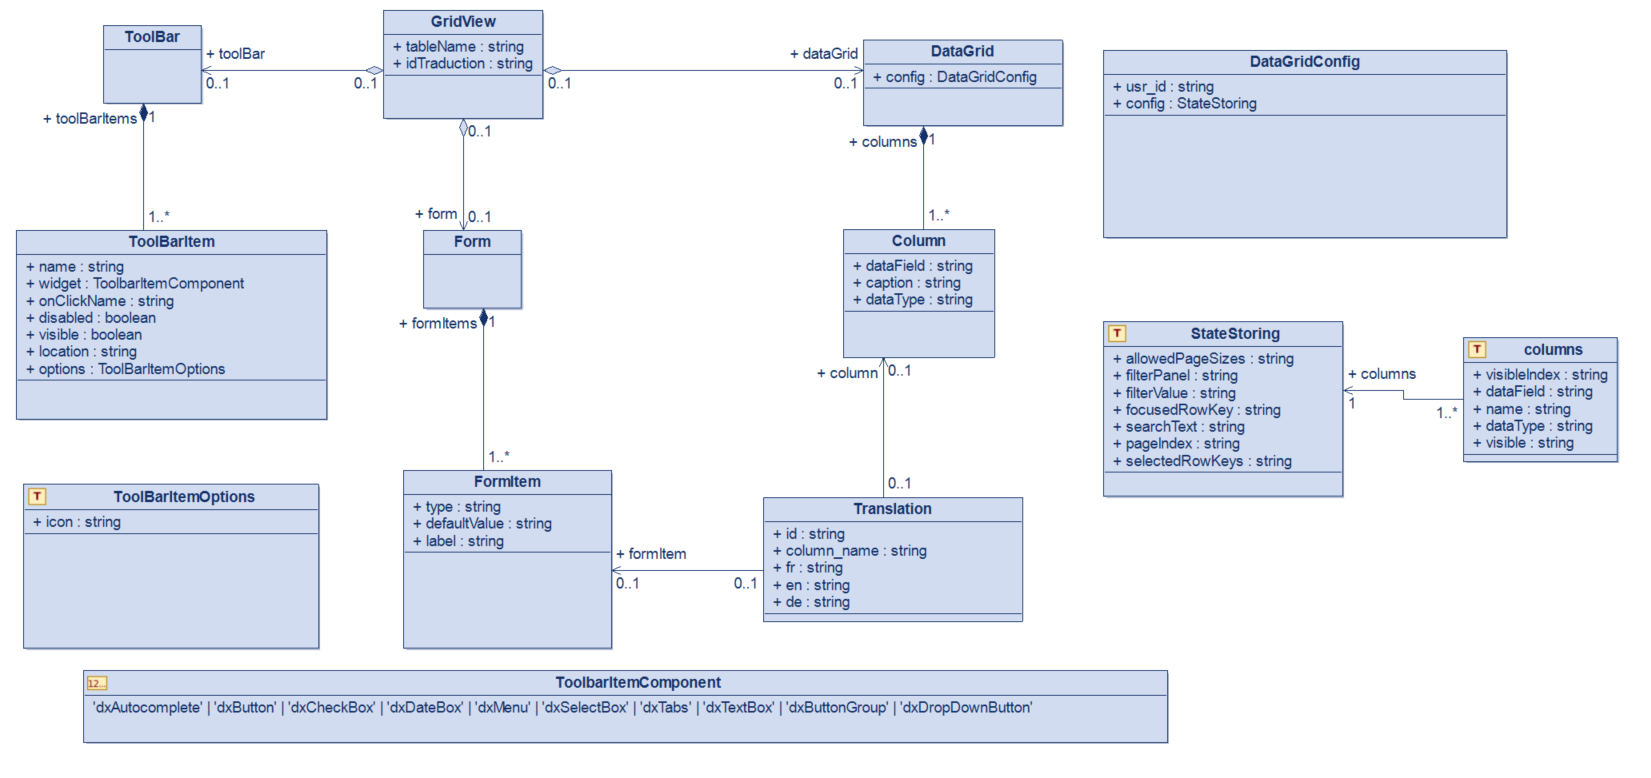
\includegraphics[width=\linewidth]{images/diagramme_classes.png}
						\end{center}
						\caption{Class diagram for storing information from a grid window}
						\floatfoot{Image source : screenshot}
						\label{fig:diagramme_classes}
					\end{figure}
					
					\noindent We will return to the achievements and results of the project in the following part.
					\newpage
				\subsection{Step \#3: Development of a \gls{backend} to interact with the database}
					Currently a lot of information useful to Morpheus is stored in a database, and not only the data displayed to users but also many management parameters of the graphical interfaces. There are also many stored procedures that allow you to perform certain actions. At the moment, we do not want to change this system, so in order to be able to access the information contained in the database, we have decided to set up a \acrshort{rest} \acrshort{api} serving as a solution \gls{backend} to the web application.\\

					As mentioned previously, Mr. NEROT had to develop a \acrshort{rest} \acrshort{api} in order to be able to communicate with the database. However, being very overloaded with his work, he did not have time to create this \acrshort{api}. So I took the initiative to develop the \acrshort{api} myself in order to test the web application with data coming from the database. This \acrshort{api} works on the \gls{crud} principle.
			
			\section{Monitoring and control}
				Monitoring and control are the pillars that ensure the consistency, quality and control of a project throughout its progress. In this section, we'll dive into the details of how we monitored and controlled my project to ensure it remained aligned with my goals and met quality standards.\\

				Monitoring and controlling are essential elements of project management because they allow you to stay on course, resolve problems in real time, and make informed decisions to ensure the success of the project. In this part, we will detail the methods, tools and practices we used to monitor progress, evaluate results and maintain the quality of my work.
				\newpage
				\subsection{Weekly meeting:"Point dev"}
					We talked about it earlier in the \ref{section:methodologie} Methodology part, the "Point dev" is a weekly meeting where each developer talks about what they did during the week. It was therefore an opportunity for me to present my work, which ensured the monitoring of the project and made it possible to check that the project was still going in the right direction.
					
				\subsection{Ad hoc follow-up meetings}
					As Managing Director France of SSI SCHAEFER, Mr GOURDON has a very busy schedule. However, it was important to him to follow the evolution of the web application development project. This is why we sometimes had occasional meetings, most often with Mr. NEROT, who allowed me to present my work to him and allowed him, if necessary, to give me his instructions on the procedure to follow to continue the project. on the right track.

		\newpage

		\part{Cyberattaque au sein de l'entreprise}
			Tout d'abord il est important de rappeler que l'entreprise SSI SCHÄFER est un groupe mondial et possède de nombreuses filiales dans plusieurs pays différents. Ainsi l'envergure du système informatique est conséquent.\\
				
				En avril 2023, l'entreprise SSI SCHÄFER a subi une cyberattaque qui a eu pour principale conséquence une coupure du système informatique complet du groupe.\\

				Bien que je n'aie personnellement pas été impacté\footnote{En effet je travaillais surtout sur mon poste en local et n'avait besoin que d'une connexion internet pour effectuer des recherches. Durant la cyberattaque j'ai donc tout simplement utilisé mon téléphone comme point d'accès avec mes données mobiles (4G et 5G)}, ou très peu, j'ai pu assiter aux conséquences qu'une telle crise peut avoir au sein d'une grande entreprise. J'ai notamment vu des collègues dans l'impossibilité compléte de pouvoir travailler.\\

				Il est aussi important de noter que le réseau informatique était coupé vers l'extérieur, et donc vers les autres sites de SSI SCHÄFER, mais nous pouvions toujours accèder aux ressources sur le réseau local de Cholet.

			\section{Impacts et conséquences}
				Les répercussions de cette cyberattaque ont été nombreuses et ont touché l'ensemble de l'entreprise, y compris sa filiale française. Dans ce contexte, je vais brièvement exposer les principales conséquences que j'ai identifiées en France.
				
				\subsection{Télétravail impossible}
					En premier lieu, tous les collaborateurs qui dépendent de l'accès à l'\acrshort{erp} de l'entreprise, particulièrement via un \acrshort{vpn}, se sont retrouvés dans l'incapacité totale d'y accéder, étant donné que la connectivité du réseau informatique de l'entreprise vers l'extérieur a été interrompue. Par conséquent, le télétravail était impossible pour eux. De plus, le serveur de messagerie était également hors service.

				\subsection{Chômage partiel}
					Effectivement, comme je l'ai mentionné précédemment, certains de mes collègues se sont malheureusement retrouvés dans l'incapacité de travailler. Ils avaient alors deux alternatives : prendre des congés pour ceux qui le pouvaient ou opter pour le chômage partiel.
					
				\subsection{Impossibilité d'aider le client}
					Étant donné que la plupart des outils d'assistance client sont normalment accessibles via le réseau informatique, il était donc impossible de fournir de l'aide aux clients de l'entreprise pendant la cyberattaque.
				
			\section{Solutions}
				\subsection{Venue des employés sur le site de Cholet}
					Bien que cette solution aurait eu sa place dans la catégorie conséquences de la cyberattaque, je tiens à la présenter ici car elle représente l'une des rares alternatives viables qui ont été envisagées. Face à l'incapacité de télétravailler, les collègues qui nécessitaient un accès à l'\acrshort{erp} se sont rendus sur le site de Cholet pour poursuivre leur travail.

				\subsection{Utilisation d'autres outils}
					Après la reprise de la connexion Internet et la réouverture de l'accès aux clients, en attendant la réactivation des \acrshort{vpn} indispensables pour se connecter, quelques solutions temporaires ont été déployées. L'utilisation de TeamViewer et Teams s'est avérée très utile pour maintenir l'assistance aux clients. Cependant, ces méthodes n'étaient pas les plus efficaces et ont rapidement été abandonnées une fois les \acrshort{vpn} rétablis.

			\section{Conclusion}
				La cyberattaque subie par SSI SCHÄFER m'a permis de prendre conscience des répercussions potentiellement dévastatrices qu'une crise majeure peut avoir au sein d'une entreprise de cette envergure. J'ai également pu constater la nécessité de faire preuve d'ingéniosité pour mettre en place des solutions, même si elles s'avèrent souvent temporaires.
			
		\newpage

		\part{Réalisations et résultats}\label{section:results}
			Au cœur de tout projet se trouvent les réalisations et les résultats qui attestent du succès et de la valeur d'une initiative. Au cours de mon stage au sein de SSI SCHÄFER, j'ai eu l'opportunité de contribuer activement à un projet qui a généré des réalisations significatives et des résultats tangibles. Dans cette section, je vais vous dévoiler ces réalisations et résultats, qui illustrent l'impact concret de notre travail sur le projet.\\

			Chacune des actions entreprises au cours de ce projet visait à atteindre des objectifs spécifiques, et ces objectifs étaient étroitement liés à la réussite de l'entreprise. Au-delà des défis et des obstacles rencontrés en chemin, ces réalisations et résultats reflètent notre engagement envers la réussite et notre capacité à transformer des idées en actions concrètes.\\

			Au fil de cette section, je vais mettre en avant les réalisations clés qui ont émergé de notre travail acharné, les résultats obtenus grâce à nos efforts collectifs, et l'impact positif de ces réalisations sur l'entreprise ou l'organisation. Je vais également illustrer comment ces réalisations ont contribué à l'atteinte des objectifs du projet.\\

			En comprenant les réalisations et les résultats de ce projet, vous aurez une vue complète de la valeur ajoutée que j'ai apportée en tant que stagiaire, ainsi que de l'impact concret de notre collaboration sur les objectifs globaux de l'entreprise. Ces réalisations témoignent de notre engagement envers l'excellence et de notre contribution à la réussite de l'entreprise.

			\section{Objectifs atteints}
				\subsection{Rappel des objectifs du projet de stage}
					Pour rappel les objectifs du projet étaient les suivants :
					\begin{itemize}
						\bdot{Tester les outils de développement}
						\bdot{Créer une maquette}
						\bdot{Créer une première version de l'\gls{app_web}}
					\end{itemize}
					
				\subsection{Tester les outils de développement}
					L'objectif initial était de tester les outils de développement \gls{tmssoftware}. Je pense que cet objectif a été parfaitement réalise. En effet au délà d'avoir tester les outils de développement. Nous avons su prouver que ce n'était pas forcément la meilleure solution et changer pour une solution plus appropriée à notre projet.

				\subsection{Créer une maquette}
					Pour cet objectif, je n'ai pas créé une maquette au sens traditionnel du terme, néanmoins à la suite du test des outils de développement nous avions une toute première version de l'\gls{app_web} qui faisait office de maquette.
				
				\subsection{Créer une première version de l'\gls{app_web}}
					Au vu des résultats du projet, je pense que nous pouvons dire que l'objectif de créer une première version de l'\gls{app_web} a été rempli.
				
			\section{Réalisations}
				\begin{figure}[ht!]
					\begin{center}
						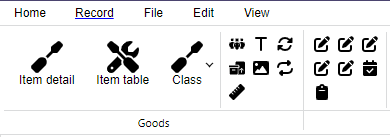
\includegraphics[width=0.7\linewidth]{images/react_menu.png}
					\end{center}
					\caption{Capture d'écran du menu de l'\gls{app_web} morpheus}
					\floatfoot{Source de l'image : capture d'écran}
					\label{fig:react_menu}
				\end{figure}
				
				\newpage
				
				\begin{figure}[ht!]
					\begin{center}
						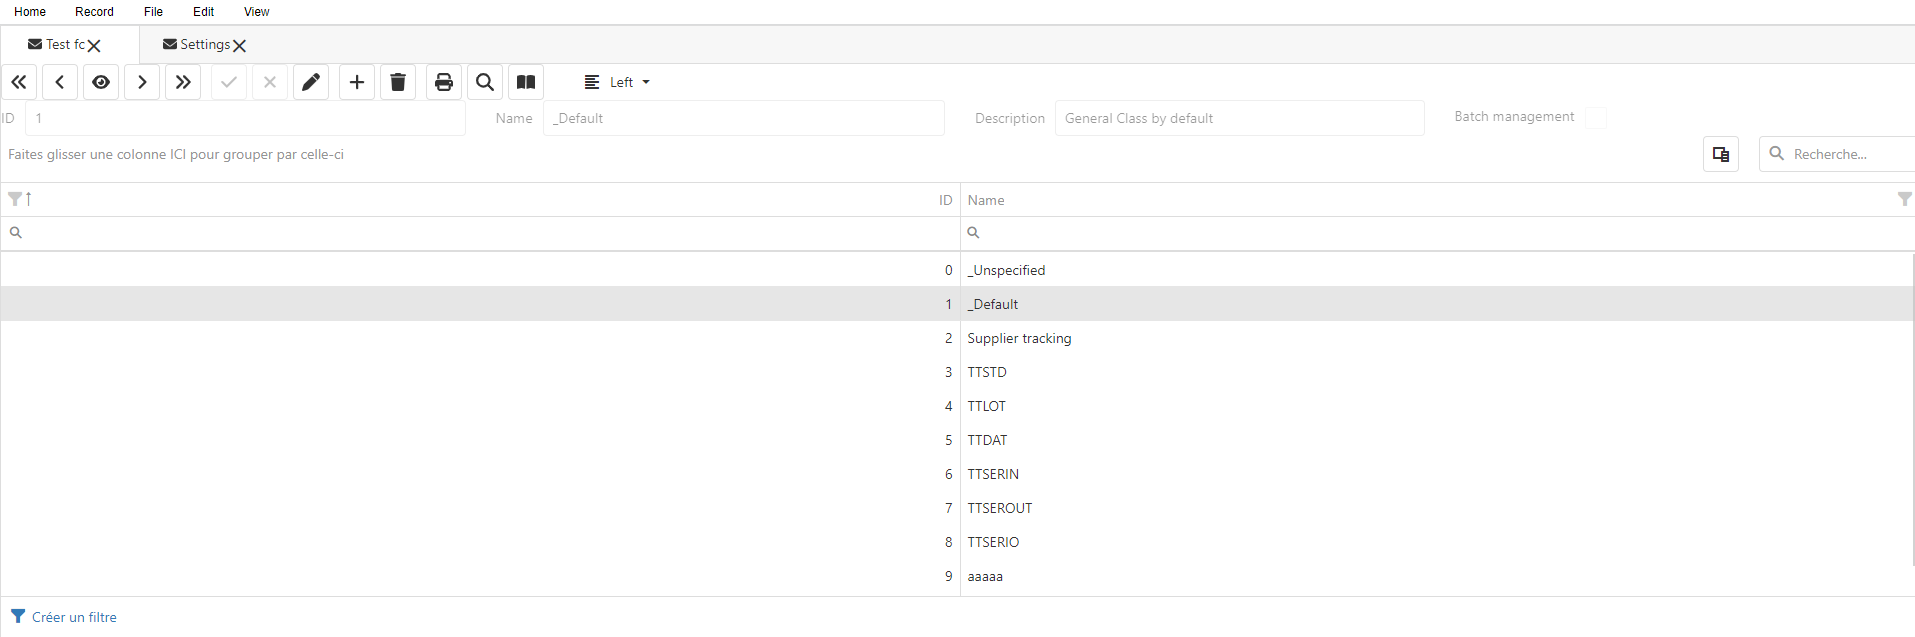
\includegraphics[width=\linewidth]{images/mph_web_reactts_1.png}
					\end{center}
					\caption{Capture d'écran de l'\gls{app_web} morpheus}
					\floatfoot{Source de l'image : capture d'écran}
					\label{fig:mph_web1}
				\end{figure}

				\begin{figure}[ht!]
					\begin{center}
						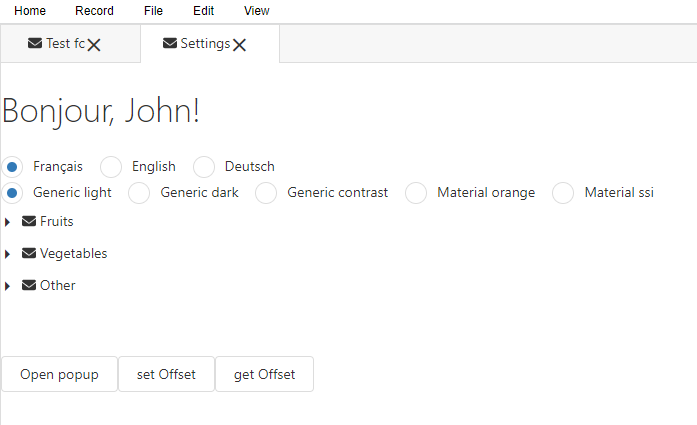
\includegraphics[width=\linewidth]{images/mph_web_reactts_2.png}
					\end{center}
					\caption{Capture d'écran de l'\gls{app_web} morpheus}
					\floatfoot{Source de l'image : capture d'écran}
					\label{fig:mph_web2}
				\end{figure}
			\newpage
			\section{Conclusion}
					En conclusion, les résultats de ce projet témoignent clairement de sa belle réussite, démontrant que j'ai atteint avec succès chacun des objectifs rigoureusement fixés. Ces objectifs, initialement tracés comme des jalons à franchir, sont désormais des réalisations concrètes. Les réalisations effectués et les retours positifs des parties prenantes confirment non seulement la réalisation de ces objectifs, mais également la création de valeurs tangibles pour l'entreprise. Cela témoigne de l'efficacité de la planification, de la gestion du projet et de l'engagement envers l'excellence qui ont été au cœur de ce projet. Les résultats obtenus fournissent une base solide pour une future reprise du projet et soulignent l'importance de la persévérance et de l'engagement à atteindre l'excellence dans la réalisation des objectifs professionnels.
		
		\newpage

		\part{Compétences mises en \oe uvre}
			Chaque expérience professionnelle, notamment un stage, est une opportunité précieuse pour développer et mettre en œuvre des compétences essentielles. Au cours de mon stage au sein de SSI SCHÄFER, j'ai eu la chance de participer activement à un projet qui m'a permis d'acquérir et de mettre en œuvre diverses compétences professionnelles de manière concrète. Cette section est dédiée à ces compétences, qui sont le socle de ma croissance en tant que professionnel.\\

			Lorsque nous évoluons dans un environnement professionnel, il est essentiel de savoir identifier, adapter et appliquer nos compétences en réponse aux défis spécifiques rencontrés. Ce projet a été le terrain d'entraînement idéal pour mettre en pratique mes compétences, tout en les renforçant et en les perfectionnant. En partageant ces compétences mises en œuvre, je souhaite démontrer comment mon stage a été bien plus qu'une simple expérience d'observation, mais une réelle occasion d'apprentissage et de croissance professionnelle.\\

			Au fil de cette section, je vais mettre en avant les compétences clés que j'ai mobilisées et développées tout au long du projet, expliquer comment elles ont été appliquées dans un contexte professionnel concret, et montrer en quoi elles ont contribué aux réalisations et au succès du projet. Ces compétences, acquises au cours de mon stage, seront sans aucun doute un atout précieux dans ma future carrière professionnelle, et je suis enthousiaste à l'idée de les développer davantage dans des contextes similaires.

			\section{Compétences techniques}
				Les compétences techniques jouent un rôle central dans notre capacité à concevoir, développer, mettre en œuvre et optimiser l'\gls{app_web} morpheus. Tout au long de cette partie, je vais mettre en lumière les compétences spécifiques que j'ai utilisées pour atteindre mes objectifs.
				\begin{itemize}
					\bdot{Développement d'une \gls{app_web} en \gls{delphi} avec l'utilisation de \gls{tmsweb}}
					\bdot{Développement d'une \gls{app_web} en \gls{html}, \gls{css} et \gls{javascript}}
					\bdot{Développement d'une \gls{app_web} en \gls{react} avec l'utilisation de typescript et du \gls{framework} \gls{devextreme}}
					\bdot{Réalisation d'un diagramme de classe}
					\bdot{Rédaction de diverses requête SQL}
					\bdot{Rédaction du présent mémoire avec Latex}
				\end{itemize}		
			
			\section{Compétences en gestion}
				La réussite de tout projet ou mission professionnelle repose non seulement sur des compétences techniques solides, mais également sur une expertise en gestion efficace. Dans cette section, nous explorerons les compétences en gestion que j'ai mises en œuvre tout au long de mon stage et comment elles ont contribué à la réalisation de mes objectifs.
				
				\subsection{Gestion du temps}
					Au cours de mon stage au sein de SSI SCHÄFER, j'ai pu faire preuve d'une bonne gestion de mon temps, en répartissant les tâches que j'avais en faire pour une semaine donnée.	

				\subsection{Planification}
					Comme tout projet d'envergure, il paraît évident de proposer une planification des différents jalons qui rythmeront l'avancée des travaux. Ainsi j'ai pu mettre en pratique mes compétences en planification en établissant un diagramme de GANTT des différentes étapes du projet de stage.
			
			\section{Compétences en communication}
				La communication efficace est le cœur de toute entreprise ou projet réussi. Dans cette section, nous allons explorer en détail les compétences en communication que j'ai utilisées et développées tout au long de mon stage et comment elles ont été essentielles pour atteindre mes objectifs.
				
				\subsection{Rédaction d'une documentation technique}			
					Un projet ne dure pas nécessaire seulement le temps d'un stage. J'ai donc dû, en parallèle de l'avancée du projet, écrire une documentation technique de celui-ci, afin qu'une personne tierce puisse reprendre et continuer le projet même après la fin de mon stage et mon départ de l'entreprise.
			
			\section{Compétences en leadership}
				Le leadership est une compétence fondamentale qui transcende les rôles et les industries. Dans cette section, nous allons explorer en détail comment ma capacité à exercer un leadership efficace a été déterminante tout au long de mon stage et comment cela a eu un impact significatif sur sa réussite.

				\subsection{Développement de l'\acrshort{api} \acrshort{rest}}
					Comme je l'ai déjà évoqué plusieurs fois au cours de ce mémoire, cela n'était, à la base, pas prévu que je développe l'\acrshort{api} \acrshort{rest} qui servirait à communiquer avec la base de données. Néanmoins, lorsque j'ai vu que la personne qui devait s'en charge, n'en avait pas le temps, j'ai alors pris l'initiative de développer ma propre version de l'\acrshort{api} afin de pouvoir continuer à avancer dans le projet.
			
			\section{Compétences en adaptabilité}
				L'adaptabilité est une compétence clé dans le monde professionnel en rapide évolution d'aujourd'hui. Dans cette section, nous allons explorer comment ma capacité à m'adapter aux changements, aux défis et aux nouvelles situations a été mise en évidence tout au long de mon stage et comment cela a contribué à sa réussite.
				
				\subsection{Choix du changement de \gls{langage_programmation}}
					Au départ du projet, l'entreprise souhaitait utiliser le \gls{langage_programmation} \gls{delphi} pour développer l'\gls{app_web}. Néanmoins je me suis vite aperçu que ce n'était pas la technologie la plus adaptée pour ce projet et ai donc suggéré que l'on utilise des technologies plus modernes qui conviendrait mieux. Après avoir présenté mes arguments auprès de monsieur NEROT et monsieur GOURDON, nous avons donc décidé que l'application serait développée en \gls{react} avec l'utlisation du \gls{framework} \gls{devextreme}.
			
			\section{Leçons apprises et développement professionnel}
				Au cours de mon stage, j'ai été constamment confrontés à une série de défis exigeants, mais aussi à des moments de réussite gratifiants. Chacun de ces moments a été une occasion d'apprentissage précieuse, contribuant à mon développement professionnel de manière significative.\\

			Une des leçons clés que j'ai tirées de cette expérience est la valeur de la résilience face à l'adversité. Lorsque nous avons été confrontés à des obstacles apparemment insurmontables, j'ai découvert une détermination et une créativité que je ne me connaissais pas. Ces moments difficiles m'ont appris que la persévérance est souvent la clé pour surmonter les défis et atteindre nos objectifs.\\

			D'autre part, mon travail m'a également montré l'importance de la communication efficace. Travailler au sein d'une équipe multidisciplinaire exigeait une communication transparente et ouverte. Apprendre à écouter activement, à exprimer mes idées de manière claire et à résoudre les conflits de manière constructive sont des compétences que j'ai affinées et que je continuerai à cultiver dans mon développement professionnel.\\

			Une autre leçon cruciale a été la valeur de la planification stratégique. Les moments où j'ai pris le temps de planifier soigneusement nos actions et de définir des objectifs clairs ont généralement été les moments où j'ai réalisé mes meilleurs résultats. Cela m'a montré que le temps consacré à une planification minutieuse est un investissement précieux pour la réussite.\\

			En réfléchissant à ces leçons et à d'autres, nous pouvons voir comment mon expérience au sein de SSI SCHÄFER a profondément influencé mon développement professionnel. Je suis convaincu que les compétences et les connaissances que j'ai acquises ici seront des atouts précieux dans mon parcours professionnel futur, me permettant de relever de nouveaux défis avec confiance et détermination. Cette expérience m'a également renforcé dans mon engagement envers l'apprentissage continu et le développement de compétences pour rester compétitifs et pertinents dans mon domaine.
	\newpage
	\phantomsection
	\part*{Abschluss\footnote{Retrouver la traduction en français de la section Conclusion en Annexe \ref{appendix:conclusion_translation} \nameref{appendix:conclusion_translation}} (Conclusion)}
	%\addcontentsline{toc}{part}{Abschluss (Conclusion)}
		Zusammenfassend hat diese Dissertation die Hauptbestandteile des komplexen und bedeutenden Prozesses des Übergangs von einer Thick-Client-Anwendung zu einer Webanwendung untersucht. Im Rahmen unserer Studie haben wir uns mit verschiedenen technischen, organisatorischen und strategischen Aspekten dieses Übergangs befasst und die mit dieser Entwicklung verbundenen Herausforderungen und Chancen hervorgehoben.\\

		Wir untersuchten zunächst den Kontext dieses Übergangs, stellten das Unternehmen SSI SCHÄFER vor und definierten die Gründe und die Motivationen, die das Unternehmen zu dieser großen Veränderung bewegten. Anschließend legten wir den theoretischen Rahmen der Dissertation fest, der es ermöglichte, die Schlüsselkonzepte zu definieren, die im gesamten Dokument Anwendung fanden. Wir haben außerdem eine vergleichende Analyse zwischen Webanwendungen und Thick-Client-Anwendungen durchgeführt, um die wesentlichen Unterschiede zwischen den beiden Ansätzen besser zu verstehen.\\

		Danach stellten wir das Projekt vor und untersuchten die Herausforderungen und Bedeutung, die es für das Unternehmen hatte. Anschließend kehrten wir zu den, während des Projekts verwendeten, Methoden und Werkzeugen zurück. Damit haben wir die Bedeutung von Planung und Projektmanagement sowie Zusammenarbeit und Kommunikation hervorgehoben. Dies ermöglichte uns auch, die eingesetzten technologischen Werkzeuge vorzustellen.\\

		Anschließend haben wir die wichtigsten Phasen des Migrationsprozesses detailliert beschrieben und dabei den Schwerpunkt auf die strategische Planung, die Auswahl der Technologien und die Entwicklung einer ersten Version der Webanwendung gelegt. Wir haben die entschei dende Bedeutung der interdisziplinären Zusammenarbeit zwischen den Beteiligten hervorgehoben, um die Projektsteuerung und -überwachung sicherzustellen und einen erfolgreichen Übergang zu ermöglichen. Durch den Cyberangriff, dem das Unternehmen ausgesetzt war, konnten wir eine Vision für das Krisenmanagement entwickeln.\\

		Abschließend untersuchten wir die konkreten Ergebnisse des Übergangs und hoben funktionale Verbesserungen hervor. Wir haben aus dieser Erfahrung auch wichtige Lehren gezogen, darunter die Bedeutung sorgfältiger Planung, transparenter Kommunikation und Anpassungsfähigkeit angesichts unvorhergesehener Herausforderungen. Außerdem konnte ich alle Fähigkeiten hervorheben, die ich während meines Praktikums anwenden, erwerben und weiterentwickeln konnte und die als Grundpfeiler für meine zukünftige berufliche Tätigkeit dienen werden.\\

		Kurz gesagt, diese Dissertation hat gezeigt, dass der Übergang von einer Thick-Client-Anwendung zu einer Webanwendung ein komplexer, aber wesentlicher Prozess ist, um in einem sich ständig weiterentwickelnden digitalen Umfeld wettbewerbsfähig zu bleiben. Er betonte auch die Bedeutung der strategischen Ausrichtung, des Teamengagements und einer eingehenden Kosten-Nutzen-Analyse. Diese Erfahrung hat uns gezeigt, dass ein Unternehmen mit sorgfältiger Planung und effektiver Umsetzung diesen Meilenstein erfolgreich meistern und sich an neue Marktanforderungen anpassen kann.\\

		Letztendlich war diese Dissertation viel mehr als nur eine technische Fallstudie, sie war ein tiefer Einblick in die, sich ständig verändernde, Welt  der Technologie, des Projektmanagements, der interdisziplinären Kommu nikation und der Anpassungsfähigkeit an Veränderungen. Darüber hinaus  beschränkt sich diese Dissertation nicht nur auf die Dokumentation eines  technologischen Wandels, sie erinnert uns auch daran, dass in der sich ständig verändernden Welt von heute Anpassungsfähigkeit, strategische Planung und Ausdauer für jedes Unternehmen von unschätzbarem Wert sind.\\

		Wie SSI SCHÄFER stehen auch wir alle vor der Notwendigkeit, uns anzupassen und innovativ zu sein, um erfolgreich zu sein. Die aus dieser Erfahrung gewonnenen Erkenntnisse sind Kompasse, die uns auf unserem eigenen Weg in die digitale Zukunft leiten können.\\

		Wenn wir die letzte Seite dieser Memoiren umblättern, sollten wir bedenken, dass unsere Erkundung gerade erst begonnen hat. Die Welt der Technologie entwickelt sich weiter, Herausforderungen tauchen auf unerwartete Weise auf und Chancen eröffnen sich für diejenigen, die bereit sind, sie zu ergreifen. Der Übergang von einer Thick-Client-Anwendung zu einer Webanwendung ist nur ein Kapitel in der sich ständig weiterentwickelnden Geschichte von Innovation und Anpassung.

	\newpage
	
	\phantomsection

	%\renewcommand{\bibname}{Bibliographie}
	%\addto{\captionsfrench}{\renewcommand{\bibname}{Bibliographie}}
	\renewcommand\refname{Bibliographie}
	%site internet morpheus à changer dire que les pages ne sont plus d'actualités...
	\bibliography{testbib}
	\bibliographystyle{ieeetr}%ieeetr %unsrt
	\addcontentsline{toc}{part}{Bibliographie}
	%\addcontentsline{toc}{section}{\bibliographyname}

	%\newpage

	%\phantomsection
	%\printindex

	\newpage

\titleformat{name=\section}{\normalfont\Large\bfseries\color{ssiBlack}}{\color{ssiRed}\rule[-1.35mm]{4.5em}{1.25em}{\color{white}\hspace{-1.65cm}\normalfont\Large\bfseries\thesection\hspace{25pt}}}{1em}{}[\color{ssiYellow}{\titlerule[4pt]}\vspace*{4pt}]

\titleformat{\subsection}{\normalfont\Large\bfseries\color{ssiBlack}}{\color{ssiYellow}\rule[-1.35mm]{4.5em}{1.25em}{\color{white}\hspace{-1.95cm}\normalfont\Large\bfseries\thesubsection\hspace{20pt}}}{1em}{}[\color{ssiYellow}{\titlerule[3pt]}\vspace*{4pt}]

\titleformat{\subsubsection}{\normalfont\Large\bfseries\color{ssiBlack}}{\color{ssiRed}\rule[-1.35mm]{4.5em}{1.25em}{\color{white}\hspace{-2.25cm}\normalfont\Large\bfseries\thesubsubsection\hspace{15pt}}}{1em}{}[\color{ssiYellow}{\titlerule[2pt]}\vspace*{4pt}]

	\phantomsection
	\appendix
	\part*{Annexes}
	%\addcontentsline{toc}{part}{Annexes}
		%si moins de 26 annexes
		\renewcommand{\thesection}{\Alph{section}}
		\counterwithin{figure}{subsection}
		\counterwithin{table}{subsection}
		%sinon
		%\renewcommand{\thesubsection}{\Roman{subsection}}

		\etocsettocstyle{\section*{Liste des annexes}}{\noindent}
		\localtableofcontents

		\newpage

		\section{Traduction de la partie Introduction}\label{appendix:introduction_translation}
			Dans le paysage numérique en constante évolution, les approches de développement logiciel s'adaptent continuellement pour répondre aux exigences en perpétuelle évolution des utilisateurs et aux avancées technologiques. Une transformation majeure s'est opérée avec le passage des applications traditionnelles en \gls{client_lourd} à des solutions basées sur le web. La montée en puissance d'Internet et la prédominance des technologies web ont incité les développeurs à explorer les possibilités et les avantages de créer des \glspl{app_web} à partir d'applications \gls{client_lourd} existantes.\\

			Ce mémoire examine en partie le processus complexe de développement d'une \gls{app_web} à partir d'un \gls{client_lourd} préexistant. Son objectif est de fournir aux développeurs un exemple de transition d'une application \gls{client_lourd} en \gls{app_web} au travers d'une étude du projet que j'ai réalisé lors de mon stage de fin d'études et des informations sur ce cheminement de transformation. La discussion abordera les défis, les méthodologies et les meilleures pratiques impliquées dans cette transformation, permettant aux ingénieurs en logiciel de naviguer avec succès dans les subtilités du processus de développement.\\
	
			Au cours de mon projet de fin d'études, j'ai eu la chance de participer à la conception d'une \gls{app_web}, lors d'une transition depuis une application \gls{client_lourd}. Cette démarche a pour but de rendre le déploiement plus rapide et de rafraîchir l'esthétique de l'interface. Cette expérience m'a motivé à approfondir ma compréhension du processus de développement d'\glspl{app_web} qui évoluent à partir d'applications \gls{client_lourd}.\\
			
			De manière habituelle, une \gls{app_web} se compose essentiellement de deux composants majeurs : le \gls{frontend}, qui se rapporte à l'interface graphique perceptible par l'utilisateur, et le \gls{backend}, qui gère l'accès à la base de données et le traitement des demandes. Dans ce scénario précis, notre application sera élaborée en séparant une partie spécifique destinée à l'interface utilisateur, qui interagira au moyen de requêtes HTTP avec une \acrshort{api} \acrshort{rest}. Cette \acrshort{api} agira comme le lien de communication avec la base de données.\\
			
			Ce document traitera de la réflexion concernant la conception d'une \gls{app_web} dérivée d'une application \gls{client_lourd}. Nous aborderons plusieurs éléments, notamment le choix du \gls{langage_programmation} et du \gls{framework}, ainsi que la mise en œuvre complète de l'application, englobant la création des interfaces graphiques.\\
			
			Pour aborder le sujet et fournir des réponses aux questions soulevées, un plan de recherche a été élaboré. En premier lieu, il était essentiel de prendre une décision éclairée concernant le \gls{langage_programmation}, posant ainsi des fondations solides. Ensuite, la création d'une nouvelle interface graphique a été entreprise. Enfin, l'intégration à la base de données via une \acrshort{api} \acrshort{rest} a été mise en œuvre pour conclure le processus.\\
			
			L'objectif d'étude réside donc dans la compréhension du processus de création d'une \gls{app_web} à partir d'une base \gls{client_lourd}, tout en identifiant les distinctions majeures entre ces deux approches.\\
			
			Pour entamer ce mémoire, nous débuterons par une présentation de l'entreprise qui m'a accueilli, à savoir SSI SCHÄFER. Ensuite, nous établirons le cadre théorique, essentiel pour appréhender les concepts clés abordés dans ce document. Par la suite, nous aborderons la section scientifique, qui se concentrera sur une analyse comparative entre les applications \gls{client_lourd} et les \glspl{app_web}.\\
	
			Nous plongerons ensuite au cœur du projet, en le présentant de manière détaillée, tout en mettant en lumière ses enjeux et son importance. Un examen approfondi de la méthodologie et des outils qui ont contribué au succès du projet suivra. Nous décrirons ensuite le déroulement du projet, en exposant les différentes étapes entreprises, et nous discuterons des défis rencontrés, des réalisations accomplies, ainsi que des résultats obtenus au cours de cette période de stage.\\
	
			Avant de conclure, nous dresserons un bilan des compétences acquises et développées au cours des six derniers mois. Enfin, en annexe, vous trouverez des informations complémentaires, suivies d'un résumé du mémoire rédigé en trois langues : français, anglais et allemand.

		\newpage

		\section{Dates importantes de l'histoire SSI SCHÄFER}\label{appendix:history}
			\begin{figure}[h!]
				\begin{center}
					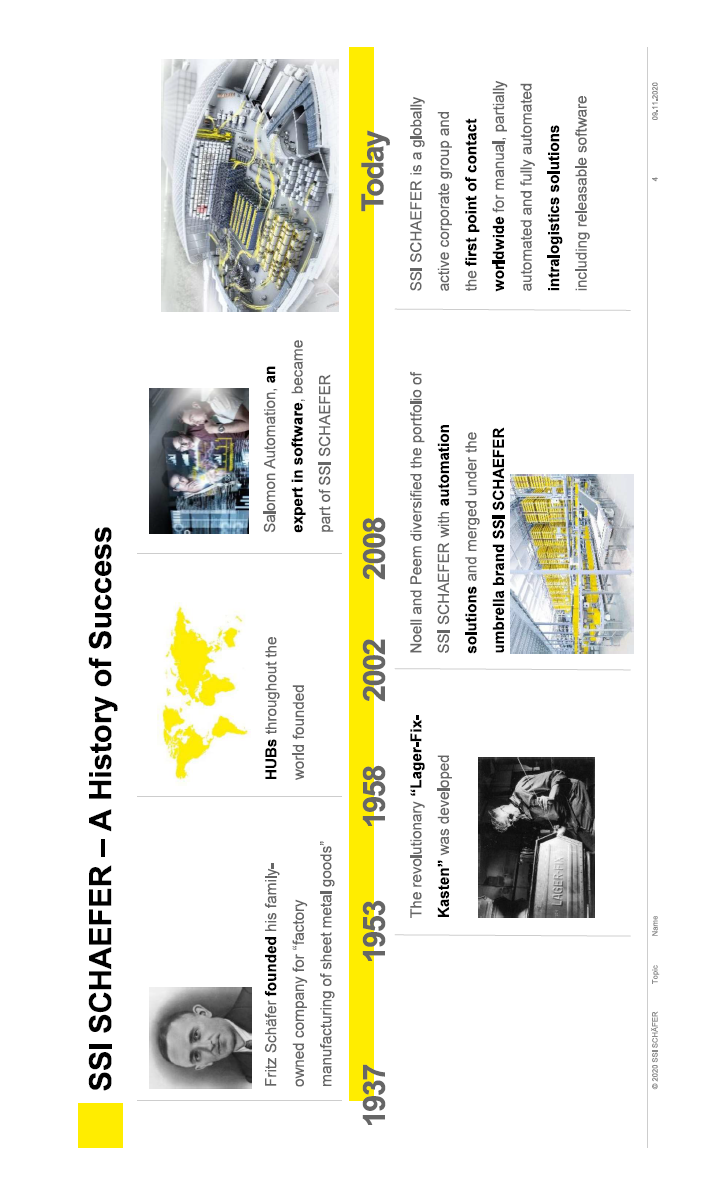
\includegraphics[width=0.7\linewidth]{images/history.png}
					\caption{Frise historique de l'histoire de SSI SCHÄFER}%\cite{screenshot}
					\floatfoot{Source de l'image : document interne}
					\label{fig:history}
				\end{center}
			\end{figure}

		\newpage
		\section{Carte des filiales SSI SCHÄFER}\label{appendix:map}
			\begin{figure}[h!]
				\begin{center}
					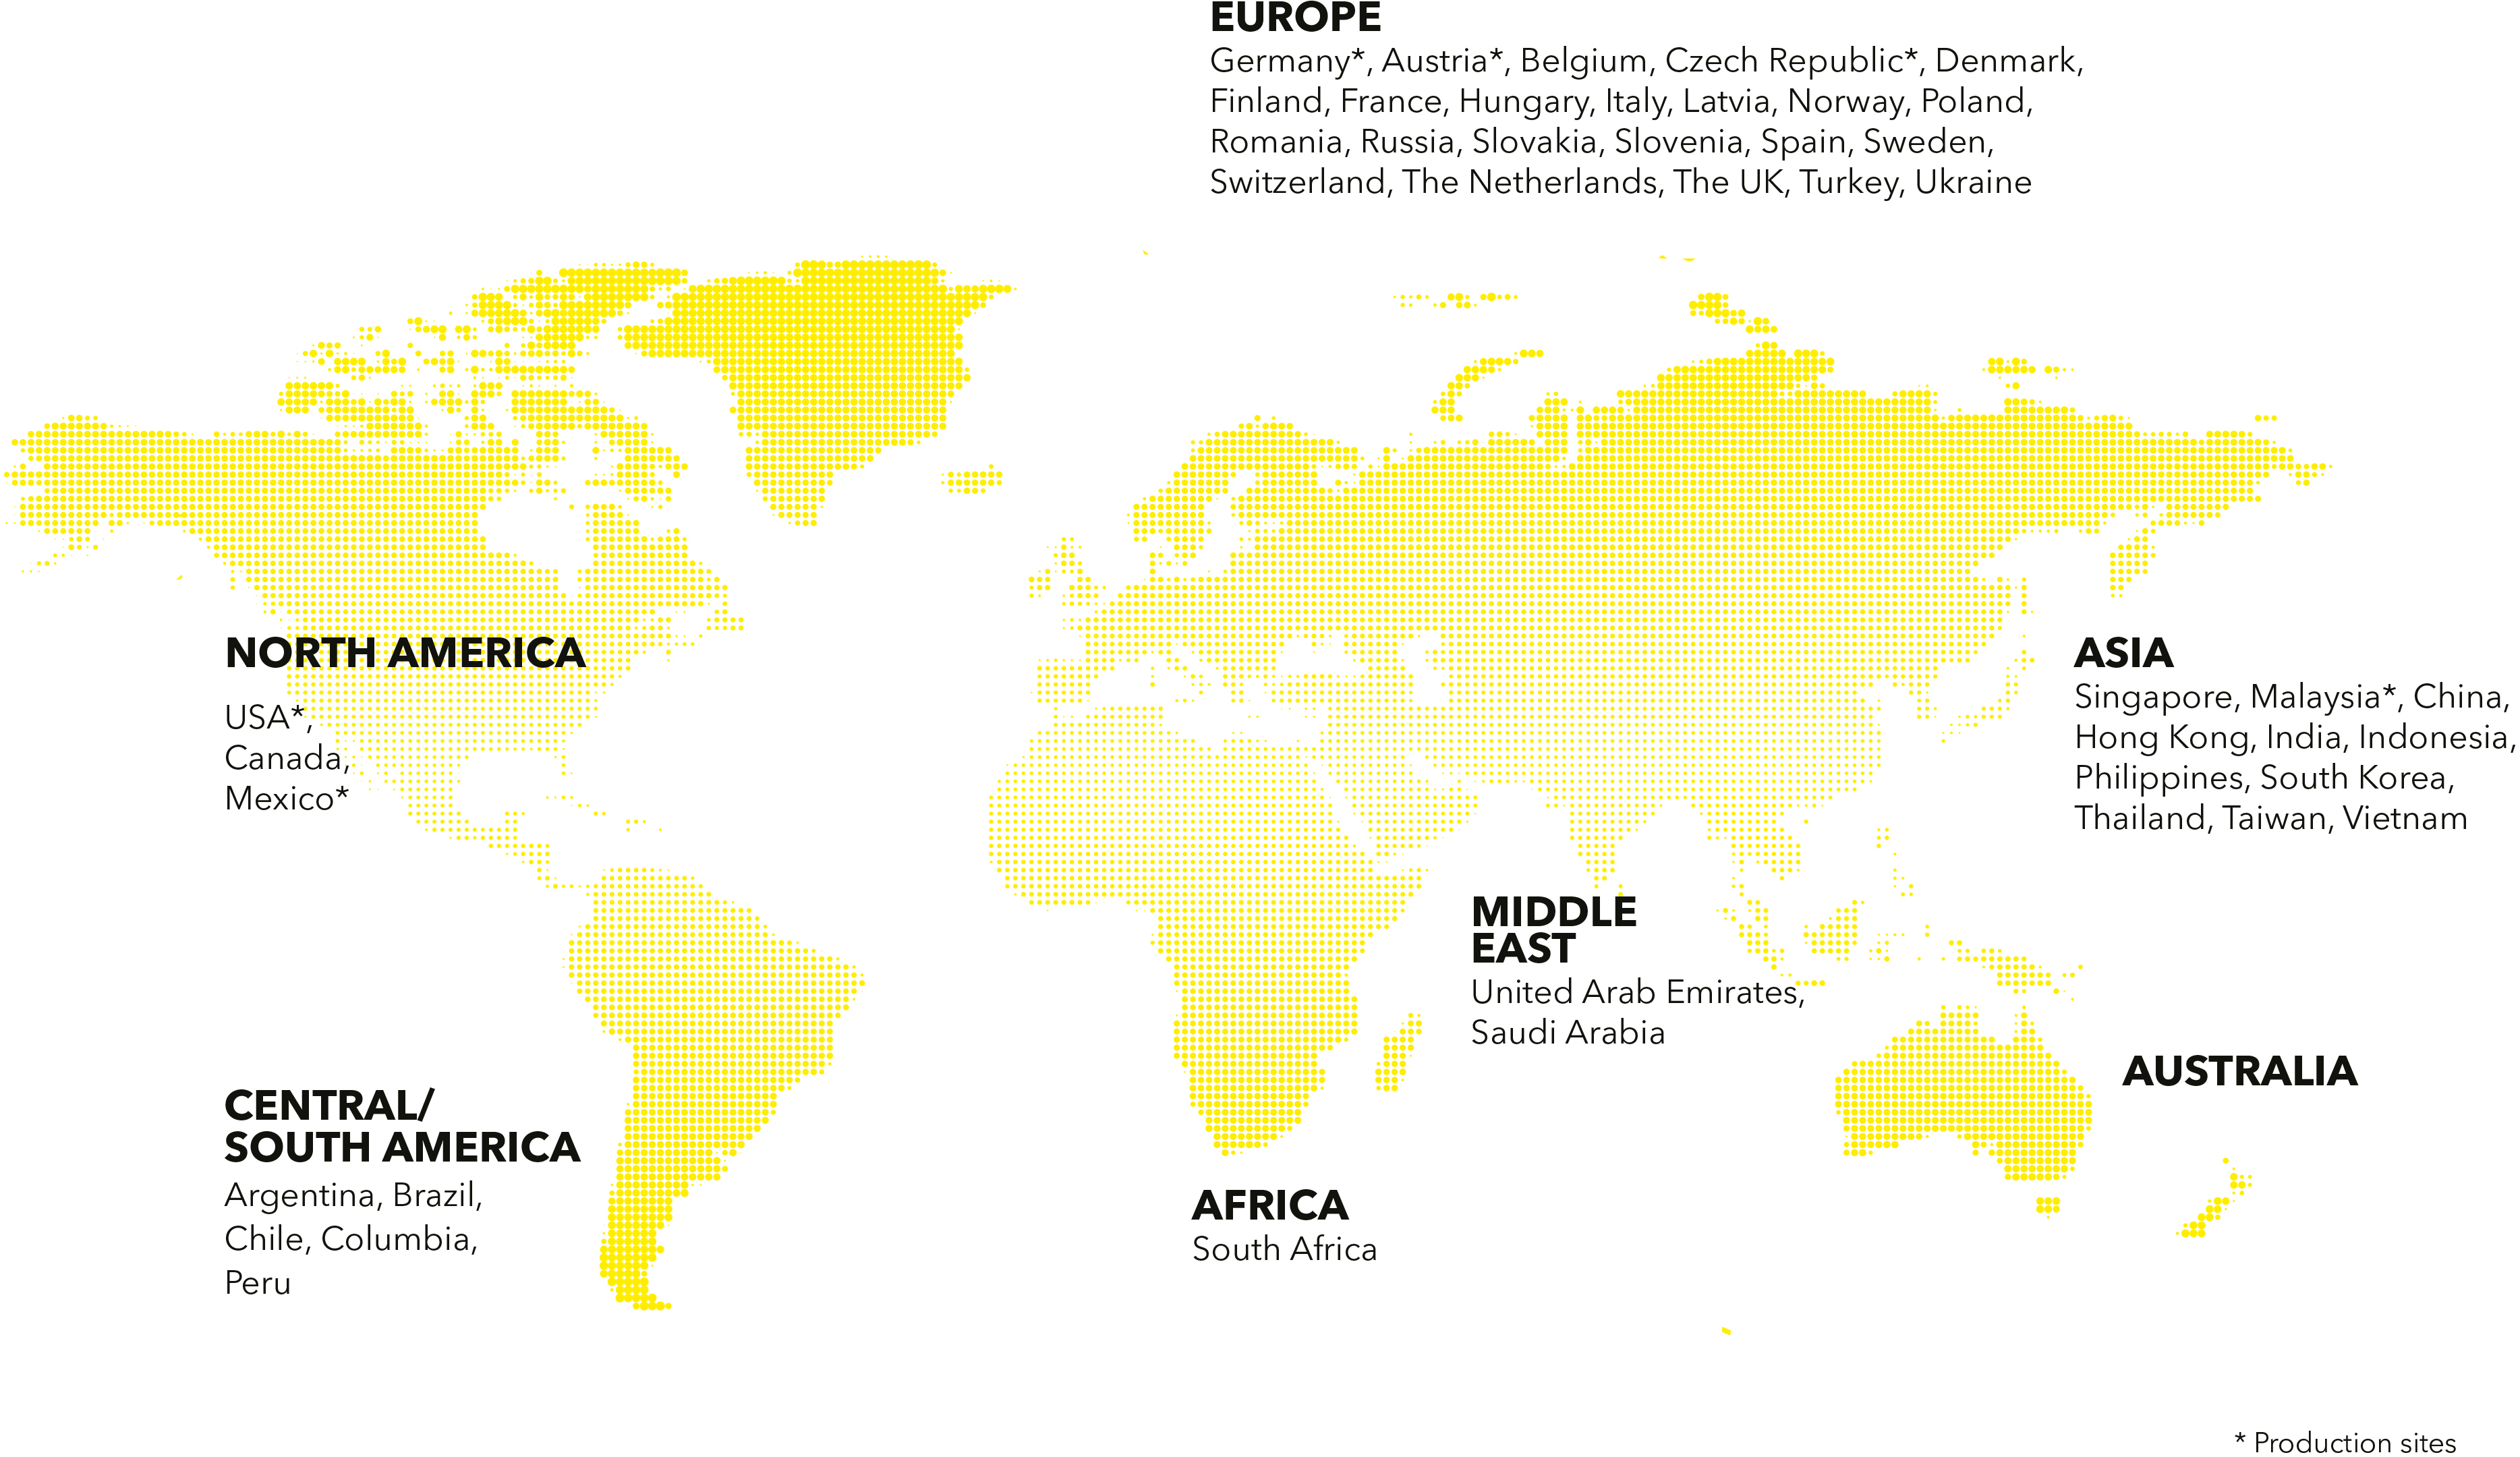
\includegraphics[width=\linewidth]{images/world_map.jpg}
					\caption{Carte des filiales SSI SCHÄFER dans le monde}%\cite{screenshot}
					\floatfoot{Source de l'image : document interne}
					\label{fig:world_map}
				\end{center}
			\end{figure}
			
		\newpage

		\section{Liste complète des fonctionnalités de MORPHEUS WMS}\label{appendix:morpheusWMSFonctionnalites}
			\begin{figure}[h!]
					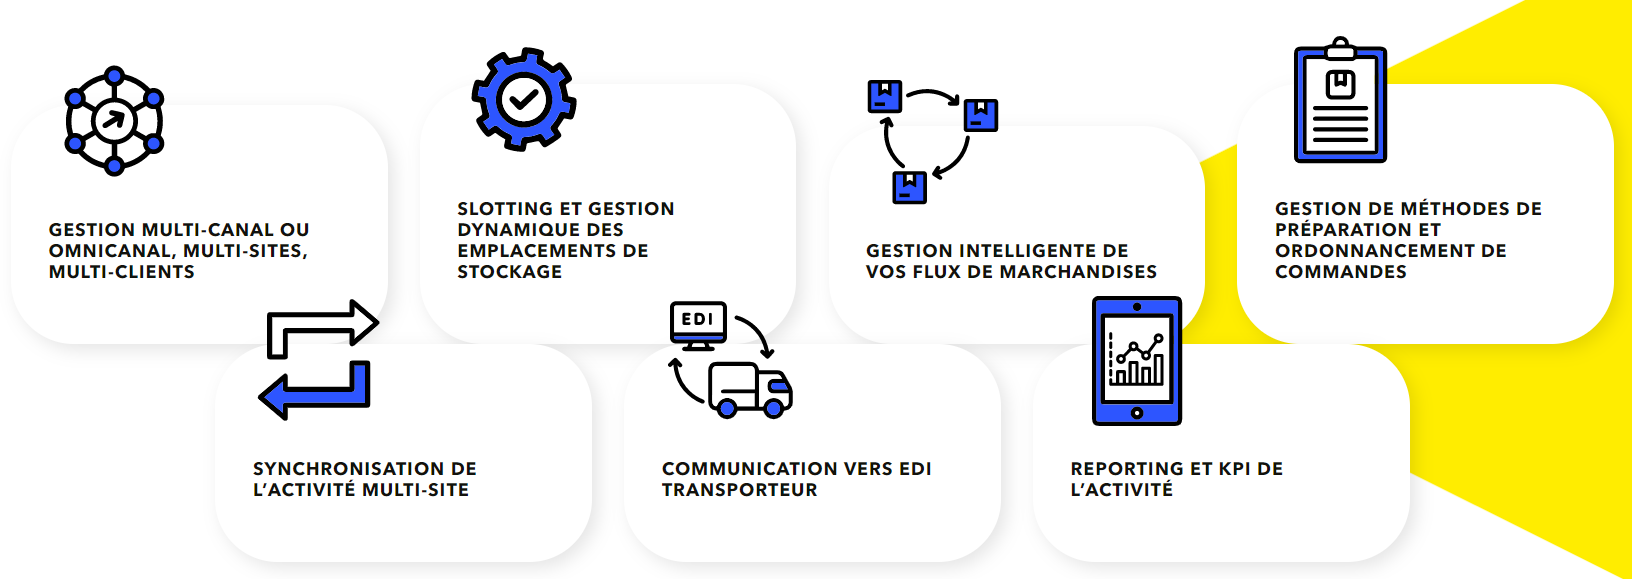
\includegraphics[width=\linewidth]{images/morpheus_wms_fonctionnalites.png}
					\caption{Fonctionnalités de Morpheus WMS}%\cite{screenshot}
					\floatfoot{Source de l'image : document interne}
					\label{fig:morpheus_wms_fonctionnalites}
			\end{figure}
		\section{Liste complète des fonctionnalités de MORPHEUS WCS}\label{appendix:morpheusWCSFonctionnalites}
			\begin{figure}[h!]
					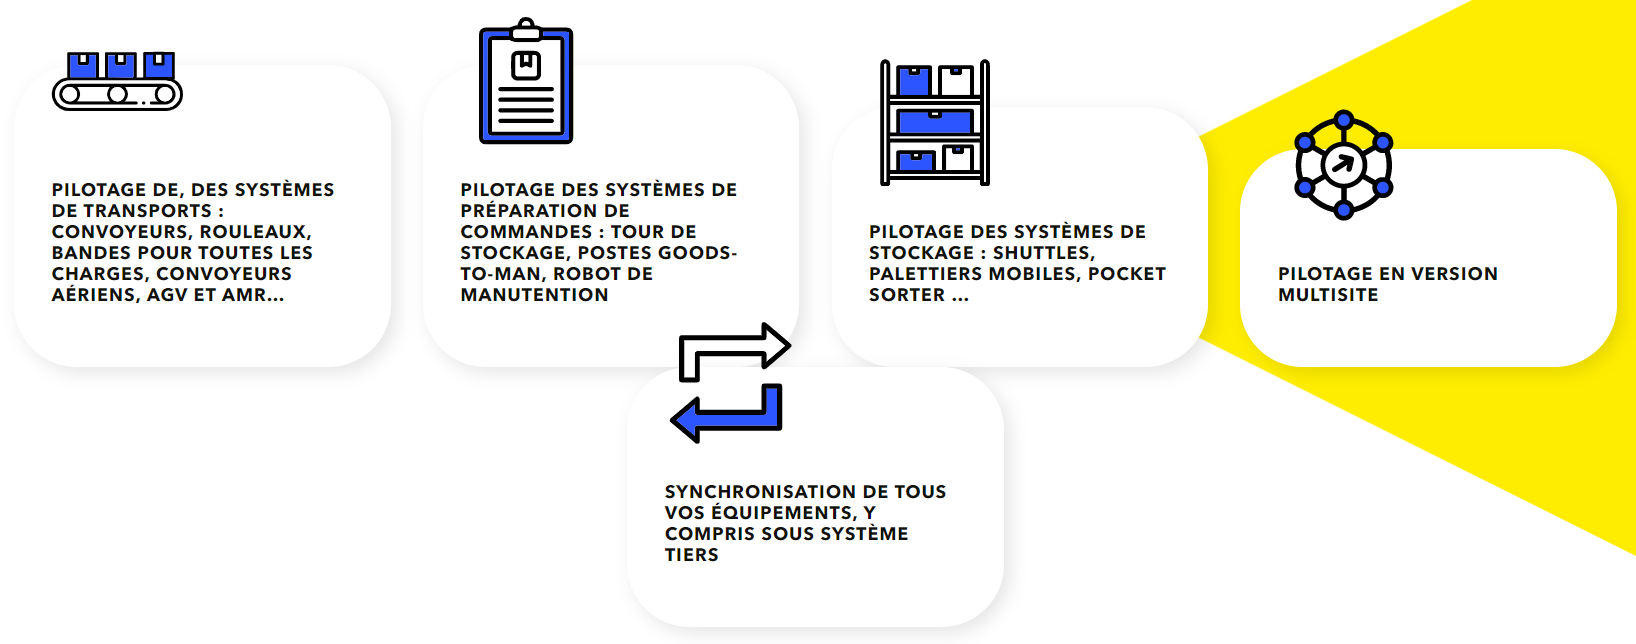
\includegraphics[width=\linewidth]{images/morpheus_wcs_fonctionnalites.png}
					\caption{Fonctionnalités de Morpheus WCS}%\cite{screenshot}
					\floatfoot{Source de l'image : document interne}
					\label{fig:morpheus_wcs_fonctionnalites}
			\end{figure}

			\newpage

		\section{Traduction de la partie Présentation du projet réalisé au cours du stage}\label{appendix_presentation_projet_translation}
			Pendant la durée de mon stage au sein de l'entreprise SSI SCHÄFER, j'ai eu l'opportunité exceptionnelle de travailler sur un projet qui a non seulement renforcé mes compétences professionnelles, mais qui a également eu un impact significatif sur l'entreprise elle-même. Dans les sections suivantes, je vais vous présenter en détail le projet que j'ai entrepris, en mettant l'accent sur son contexte, ses objectifs, les défis rencontrés et les solutions mises en place. Au fil de ce mémoire, je vous invite à découvrir les étapes que j'ai parcouru au cours de ce stage, ainsi que les résultats concrets que j'ai obtenus. Ce projet représente non seulement une expérience enrichissante pour moi, mais il témoigne également de la capacité de collaboration et d'innovation au sein de l'équipe de développeurs de SSI SCHÄFER.
		
			\subsection{Projet global}
				À l'heure actuelle, Morpheus est une suite de logiciels regroupés au sein d'un \gls{client_lourd} développé en \gls{delphi}. Cela implique que si nous voulons utiliser Morpheus, nous devons l'installer sur la machine sur laquelle nous en avons besoin ce qui peut être parfois contraignant, surtout lorsque l'on a que des opérations de gestion à faire. Ainsi afin de simplifier l'accès à Morpheus, et ce sans avoir à installer de \gls{client_lourd}, il a été décidé de développer une \gls{app_web} qui permettra d'accéder à Morpheus depuis n'importe quel poste ayant un navigateur internet. Par ailleurs, en parallèle du projet de développer une version web du client Morpheus, un projet de refonte du \gls{client_lourd} a aussi été lancé. Le but du projet n'est donc pas de remplacer un \gls{client_lourd} par une \gls{app_web} mais d'offrir plusieurs possibilités aux utilisateurs en fonction des besoins de chacun. Un manager n'a pas besoin d'accéder aux mêmes fonctionnalités qu'un technicien et vice versa.
			\newpage
			\subsection{Projet du stage}
				Bien entendu il est impossible de développer une \gls{app_web} entière qui reproduirait le comportement de Morpheus en seulement six mois de stage. C'est pour cela que durant mon stage j'ai seulement réalisé une partie du projet de création de l'\gls{app_web}. Ainsi le projet du stage était donc de tester plusieurs outils et langages de programmation, déterminer lequel serait le mieux dans notre cas et développer une première version de l'\gls{app_web}.

			\subsection{Application existante}
				Nous avons vu dans l'analyse comparative que dans la majorité des cas les \glspl{client_lourd} n'ont pas de dépendance à une connectivité réseau, néanmoins cela n'est pas une vérité générale et c'est le cas pour Morpheus. En effet la logistique étant un milieu très précis, les opérations doivent être effectuées en temps réel, ainsi l'application a besoin en permanence d'accéder à la base de données. Il est important de comprendre que de nombreuses informations sont stockés dans la base de données et sont nécessaires au bon fonctionnement de Morpheus.\\

			\noindent Voici quelques captures d'écran du logiciel Morpheus à l'heure actuelle.

				\begin{figure}[ht!]
					\begin{center}
						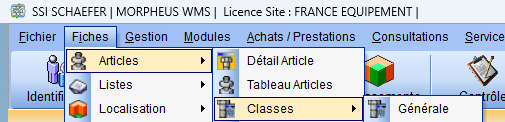
\includegraphics[width=0.7\linewidth]{images/mph_menu.png}
					\end{center}
					\caption{Partie du menu de l'application existante Morpheus}
					\floatfoot{Source de l'image : capture d'écran}
					\label{fig:mph_menu}
				\end{figure}

				\newpage

				\begin{figure}[ht!]
					\begin{center}
						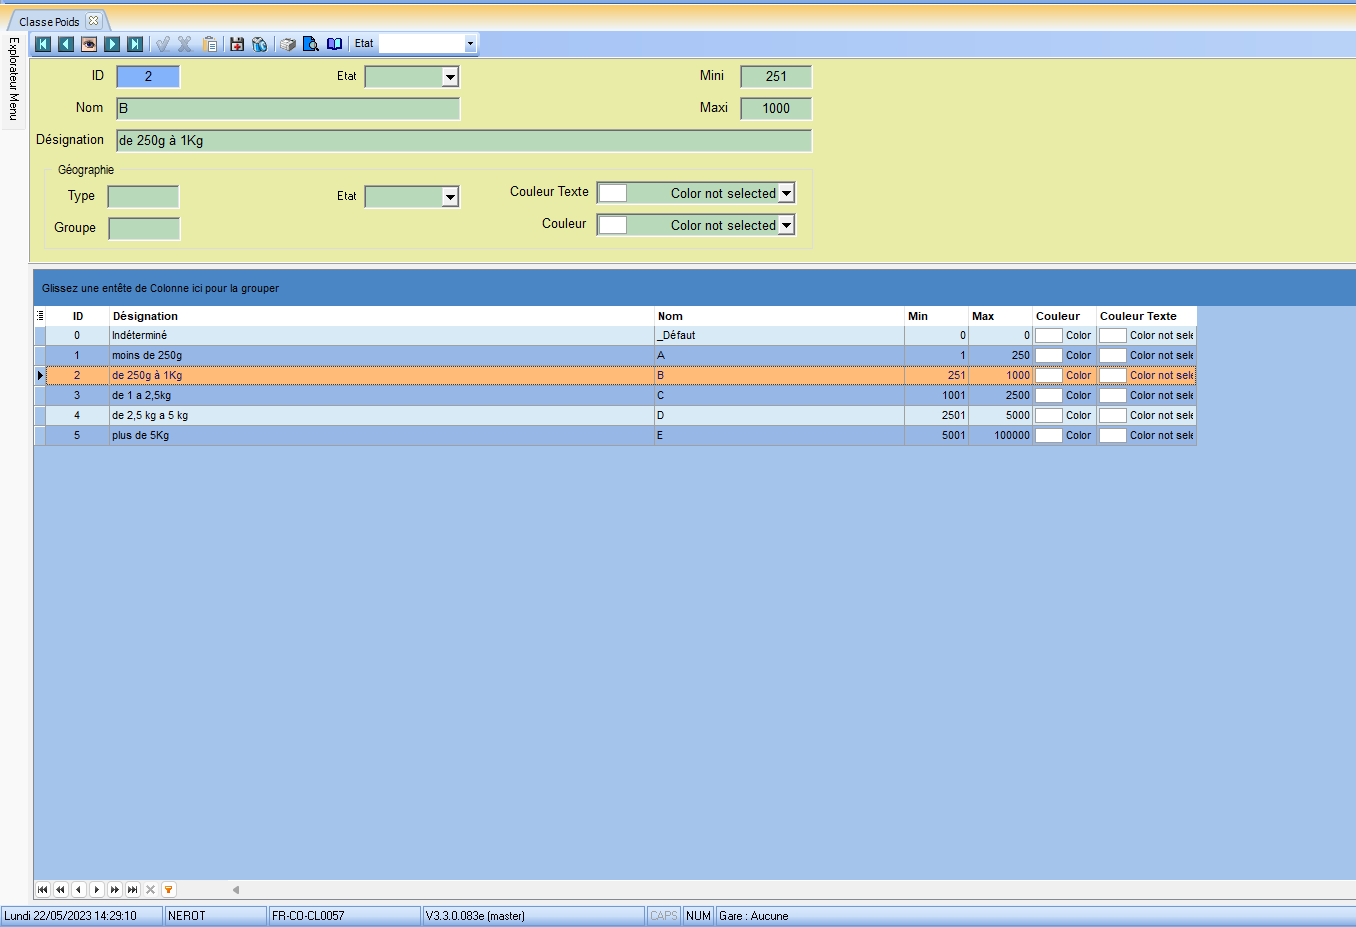
\includegraphics[width=0.7\linewidth]{images/mph_window.png}
					\end{center}
					\caption{Exemple d'une fenêtre de l'application existante Morpheus}
					\floatfoot{Source de l'image : capture d'écran}
					\label{fig:mph_window}
				\end{figure}

				Bien que le client Morpheus regroupe de nombreuses fonctionnalités, il commence à devenir ancien. Ainsi le projet de développement de l'\gls{app_web} lui offrir aussi une seconde jeunesse avec des interfaces graphiques renouvelées. De plus les managers pourront effectuées leurs opérations de gestion directement depuis leur navigateur et n'auront plus besoin d'installer le \gls{client_lourd}.

		\newpage
		\section{Traduction de la partie Déroulement du projet}\label{appendix:projet_translation}
			Le succès d'un projet repose non seulement sur son objectif et ses outils, mais également sur la manière dont il est planifié, exécuté et géré tout au long de son cycle de vie. Au cours de mon stage au sein de SSI SCHÄFER, j'ai eu l'opportunité de participer à un projet d'envergure qui a nécessité une planification minutieuse et une exécution rigoureuse. Dans cette section, je vais vous plonger dans le déroulement complet de ce projet, en décrivant les différentes étapes que j'ai suivies.

			\subsection{Objectifs et planification initiale}
				La clarté des objectifs et la planification méthodique sont les fondements de tout projet réussi. Dans cette section, nous allons explorer les objectifs que je me suis fixés au début de mon projet et la planification initiale qui a guidé mes actions.\\

				Le processus de définition des objectifs est une étape fondamentale dans la réalisation de tout projet. Dans cette partie, nous allons détailler ces objectifs, expliquer pourquoi ils ont été choisis, et comment ils étaient alignés sur les enjeux et les besoins que nous avons identifiés précédemment.\\

				La planification initiale est tout aussi essentielle. Elle nous permet de définir la trajectoire du projet, d'identifier les étapes clés, les ressources nécessaires, et de fixer des échéances réalistes. Dans cette section, je vais présenter le plan initial que j'avais mis en place.\\

				En comprenant ces éléments, vous aurez une vue d'ensemble claire de la manière dont mon projet a été conçu et structuré pour atteindre des objectifs spécifiques, tout en tenant compte des contraintes et des réalités du terrain. Cette partie jettera les bases pour la suite du mémoire, où je détaillerai la mise en œuvre et les résultats par rapport à ces objectifs initiaux.
				\newpage
				\subsubsection{Objectifs détaillés}
				\noindent Les objectifs initiaux du projet étaient les suivants :
	
					\begin{itemize}
						\bdot{Développer un client morpheus full \gls{html}5 responsive pour une partie des fenêtres du client morpheus existant}
						\bdot{Expérimenter les outils de développement \gls{tmsweb}}
						\bdot{Faire une maquette d'interface utilisateur}
							\begin{itemize}
								\bdotoutlined{Fenêtre principale}
									\begin{itemize}
										\bsquare{Menu}
											\begin{itemize}
												\bsquareoutlined{Icones}
												\bsquareoutlined{Style (comme style windows : couleurs)}
												\bsquareoutlined{X niveaux et sous niveaux paramétrables}
													\begin{itemize}
														\bdiamond{Par rapport à une bdd afficher ou pas des points d'entrées du menu}
													\end{itemize}
											\end{itemize}
										\bsquare{Boutons de fonction}
											\begin{itemize}
												\bsquareoutlined{Style}
												\bsquareoutlined{Icones}
												\bsquareoutlined{Taille des boutons (16, 32 or 48)}
												\bsquareoutlined{Rendre visible ou non les boutons}
												\bsquareoutlined{Mise en page des boutons en fonction du nombre : alignements...}
											\end{itemize}
										\bsquare{Treeview}
											\begin{itemize}
												\bsquareoutlined{Style}
												\bsquareoutlined{Icones (devant nom sans toucher au petit triangle)}
												\bsquareoutlined{Afficher une liste sur un niveau suivant une requête}
												\bsquareoutlined{Charger les arborescences dynamiques (si on clique sur site afficher les sites et pas avant)}
													\begin{itemize}
														\bdiamond{Paramétrage visible ou non des arborescences}
													\end{itemize}
											\end{itemize}
									\end{itemize}
								\bdotoutlined{Gestion des styles}
								\bdotoutlined{Gestion multi-fenêtres mdi (tabs)}
									\begin{itemize}
										\bsquare{Icones}
										\bsquare{Fermable ou non par une croix}
									\end{itemize}
								\bdotoutlined{Gestion fenêtres modales}
									\begin{itemize}
										\bsquare{Rendre visible la croix pour fermer la fenêtre ou non}
										\bsquare{Mémorisation de la position}
									\end{itemize}
								\bdotoutlined{Login}
								\bdotoutlined{Connexion à la base de données}
							\end{itemize}
						\bdot{Rédiger un descriptif du mode de fonctionnement du client au niveau ergonomique}
						\bdot{Développer une première version avec les fenêtres de base}
							\begin{itemize}
								\bdotoutlined{Fenêtre principale}
									\begin{itemize}
										\bsquare{Menu}
											\begin{itemize}
												\bsquareoutlined{Icones}
												\bsquareoutlined{Style ( comme style windows : couleurs)}
												\bsquareoutlined{X niveaux et sous niveaux paramètrables}
													\begin{itemize}
														\bdiamond{Par rapport à une bdd afficher ou pas des points d'entrées du menu}
													\end{itemize}
											\end{itemize}
										\bsquare{Boutons de fonction}
											\begin{itemize}
												\bsquareoutlined{Style}
												\bsquareoutlined{Icones}
												\bsquareoutlined{Taille des boutons (16, 32 or 48)}
												\bsquareoutlined{Rendre visible ou non les boutons}
												\bsquareoutlined{Mise en page des boutons en fonction du nombre : alignements...}
											\end{itemize}
										\bsquare{Treeview}
											\begin{itemize}
												\bsquareoutlined{Style}
												\bsquareoutlined{Icones (devant nom sans toucher au petit triangle)}
												\bsquareoutlined{Afficher une liste sur un niveau suivant une requête}
												\bsquareoutlined{Charger les arborescences dynamiques (si on clique sur site afficher les sites et pas avant)}
													\begin{itemize}
														\bdiamond{Paramétrage visible ou non des arborescences}
													\end{itemize}
											\end{itemize}
									\end{itemize}
								\bdotoutlined{Gestion des styles}
								\bdotoutlined{Gestion multi-fenêtres mdi (tabs)}
									\begin{itemize}
										\bsquare{Icones}
										\bsquare{Fermable ou non par une croix}
									\end{itemize}
								\bdotoutlined{Gestion fenêtres modales}
									\begin{itemize}
										\bsquare{Rendre visible la croix pour fermer la fenêtre ou non}
										\bsquare{Mémorisation de la position}
									\end{itemize}
								\bdotoutlined{Login}
								\bdotoutlined{Connexion à la base de données}
								\bdotoutlined{Gestion des droits d'accès}
								\bdotoutlined{Gestion paramétrage en \gls{XML} des fenêtres}
									\begin{itemize}
										\bsquare{Type de fenêtre}
										\bsquare{Grid associé}
										\bsquare{Requête sql}
									\end{itemize}
							\end{itemize}
					\end{itemize}

				\subsubsection{Planification initiale}
					Nous en avons déjà parlé un peu plutôt voici la planification des tâches initiales:
					\begin{itemize}
						\bdot{Installation et configuration des outils}
						\bdot{Expérimentation des outils}
						\bdot{Rédaction détaillée des besoins}
						\bdot{Développement du nouveau client \gls{html}5}
						\bdot{Test et recettage du nouveau client}
						\bdot{Livraison}
					\end{itemize}
						
			\subsection{Étapes du projet}
				La réalisation d'un projet réussi nécessite un plan solide et une exécution méthodique. Dans cette section, nous allons explorer les étapes clés qui ont jalonné mon parcours, du début à la fin du projet. Cette chronologie nous permettra de comprendre la séquence logique de mon travail et les accomplissements qui ont marqué chaque phase.\\

				La gestion des étapes d'un projet est essentielle pour assurer la cohérence, l'efficacité et la maîtrise des délais. Chaque étape représente un ensemble spécifique de tâches, d'objectifs et de livrables qui nous rapprochent de la réalisation de notre mission globale. Au cours de cette section, nous allons détailler ces étapes et expliquer comment elles étaient alignées sur les objectifs initiaux.

				\subsubsection{Étape n°1 : Choix du \gls{langage_programmation} pour le \gls{frontend}}
					L'application front-end de l'\gls{app_web} Morpheus est sans doute la plus importante du projet. En effet, elle représente la partie interface graphique et sera donc celle avec laquelle l'utilisateur va interagir. Il parait donc logique que la première étape du projet soit de choisir le \gls{langage_programmation} le plus adapté pour développer cette application.
	
					\paragraph{Solutions possibles\\}
						Trois principales solutions ont été envisagées pour convenir aux objectifs de ce projet. Nous allons voir quelles sont ces solutions et pourquoi elles ont été envisagées.
						
						\subparagraph{\gls{delphi} et \gls{tmssoftware}\\}
							\gls{delphi} et \gls{tmssoftware} ont été la première solution envisagée dans ce projet. En effet le langage \gls{delphi}
							 étant déjà utilisé au sein de l'entreprise SSI Schäfer, il a été logique pour eux de me proposer de réaliser le projet en utilisant cet outil. Néanmoins, je me suis très vite rendu compte que cela n'allait pas être l'outil le plus adapté pour notre projet d'\gls{app_web}.\\

								\noindent Retrouvez une présentation du résultat obtenu avec \gls{delphi} en Annexe \ref{appendix:delphi_result} \nameref{appendix:delphi_result}.\\
								\noindent Retrouvez un exemple de code produit en \gls{delphi} en Annexe \ref{appendix:delphi_code} \nameref{appendix:delphi_code}.
											
						\subparagraph{\gls{javascript}\\}
							\gls{javascript} a été la deuxième option à laquelle j'ai pensé pour faire ce projet. En effet, voyant que \gls{delphi} ne serait pas la solution la plus adaptée, j'ai commencé à développer une \gls{app_web} en \gls{javascript} vanilla. Les premiers résultats m'ont plutôt satisfait mais j'ai vite compris que si je devais redévelopper tous les composants dont j'avais besoin cela prendrait beaucoup trop de temps. Il me fallait donc trouver un \gls{framework} \gls{javascript} qui me donnerait accès aux composants dont j'avais besoin.
					
						\subparagraph{\gls{react} et \gls{devextreme}\\}
							Après reflexion et échange avec Monsieur NEROT, nous avons pensé que \gls{react} pourrait être une bonne solution pour développer l'\gls{app_web} Morpheus. Néanmoins il nous fallait aussi trouver un \gls{framework} capable de nous fournir les composants graphiques donc nous avions besoin. C'est là que nous avons pensé à \gls{devextreme}. En effet l'entreprise utilise déjà des \glspl{framework} \gls{devexpress} pour le développement du \gls{client_lourd} morpheus. Suite à un échange avec Monsieur GOURDON, il nous a indiqué qu'il existait un \gls{framework} pour \gls{javascript}. Nous nous sommes donc renseignés sur celui et avons décidé de tester ce que nous pourrions faire avec celui-ci.\\		
					
					\noindent Retrouvez un exemple de code produit en \gls{react} et \gls{devextreme} en Annexe \ref{appendix:react_code} \nameref{appendix:react_code}\footnote{Vous pourrez avoir un aperçu des résultats produits en react et \gls{devextreme} dans la section \ref{section:results} \nameref{section:results}}.
		
						\paragraph{Solution retenue\\}
							Ainsi à la lumière des tests réalisés dans les différents langages/\glspl{framework} ainsi que le comparatif technique entre \gls{tmsweb} et \gls{devextreme}\footnote{Retrouvez le comparatif technique entre les solutions \gls{tmsweb} et \gls{devextreme} en Annexe \ref{appendix:tms_devextreme} \nameref{appendix:tms_devextreme}}, nous avons choisi de retenir la solution \gls{react} + DevExtreme. En effet nous avons établi que la solution \gls{react} + \gls{devextreme} était plus adapté à notre projet du fait de sa flexibilité accrue pour le multiplateformes ainsi qu'une large gamme de widgets modernes.

							\subparagraph{Impact financier\\}
								L'avantage du \gls{framework} \gls{devextreme}, comparé à d'autres \glspl{framework}, est qu'on peut l'utiliser pour développer sans avoir à payer. Cela est un avantage car si on se rend compte que le \gls{framework} n'est pas le bon, nous n'avons pas payer un \gls{framework} pour rien. Mais cela reste très compliqué de chiffre le gain d'argent que peut procurer l'utilisation d'un \gls{framework} par rapport à un autre, car ce n'est pas la seule variante à prendre en compte. En effet l'expérience du développeur ou même la complexité du projet peuvent être des facteurs importants.
				\newpage	
				\subsubsection{Étape n°2 : Développement de la première version du \gls{frontend}}
					Après avoir choisi le \gls{langage_programmation} avec lequel nous voulions travailler, j'ai commencé à développer la première version du \gls{frontend} de l'\gls{app_web}. Ainsi la première étape était de créer un menu pour pouvoir naviguer dans les différentes fenêtres du client web morpheus. Puis j'ai développé une fenêtre type avec une grille.\\
					
					Voici le diagramme de classe que j'ai réalisé afin de stocker les informations d'une fenêtre type grille. Cette partie est liée à la création de l'\acrshort{api} qui interragit avec la base de données. Néanmoins il était préférable de commencer à réfléchier aux informations que l'on veut stocker dans la base de données dès la création du \gls{frontend}.

					\begin{figure}[ht!]
						\begin{center}
							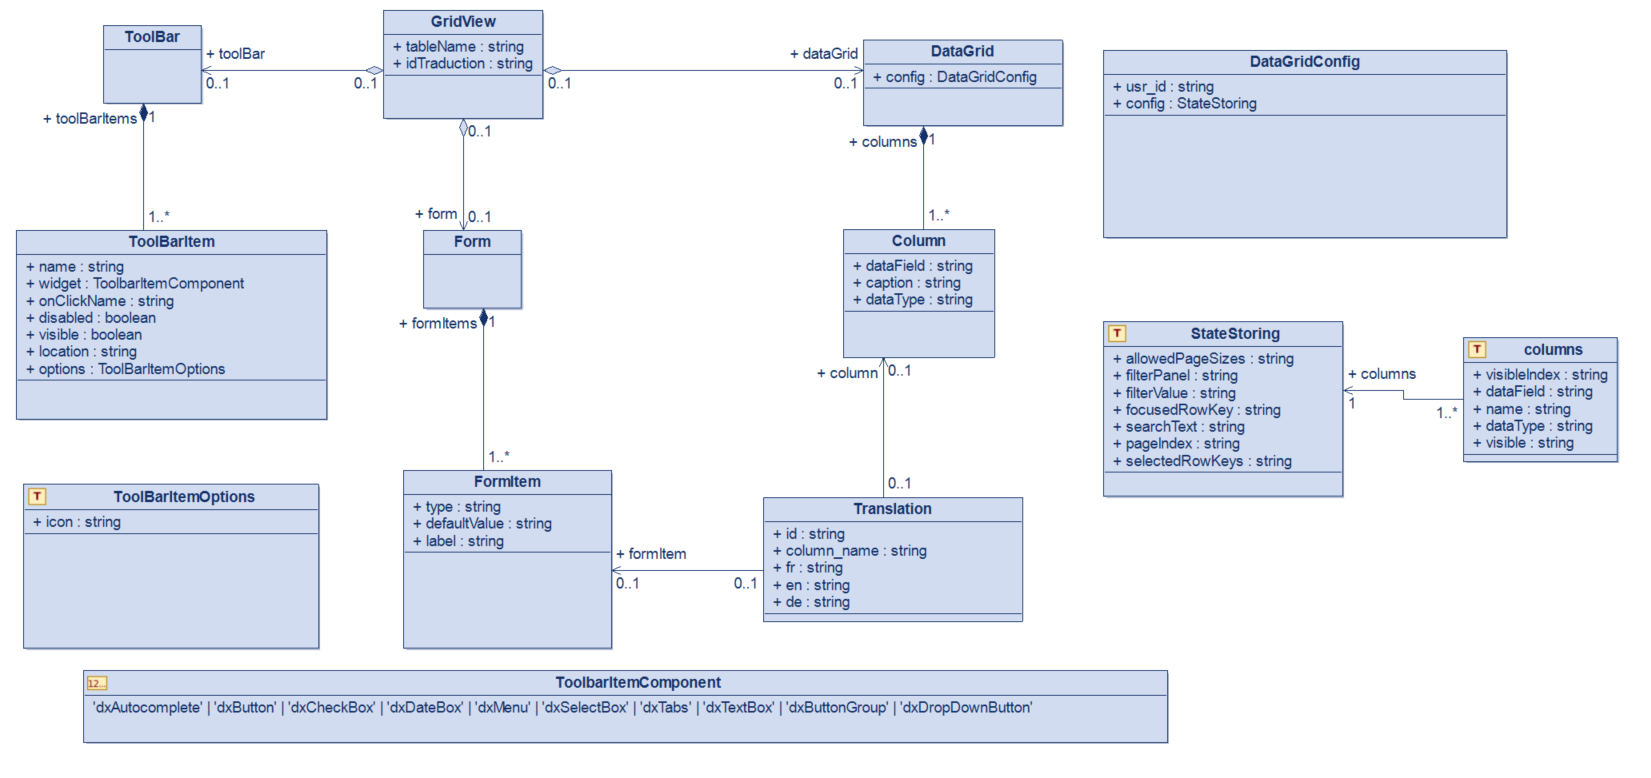
\includegraphics[width=0.7\linewidth]{images/diagramme_classes.png}
						\end{center}
						\caption{Diagramme de classe pour le stockage des informations d'une fenêtre type grille}
						\floatfoot{Source de l'image : capture d'écran}
						\label{fig:diagramme_classes}
					\end{figure}
					
					\noindent Nous reviendrons sur les réalisations et les résultats du projet dans la section suivante.
				\newpage
				\subsubsection{Étape n°3 : Développement d'un \gls{backend} pour intéragir avec la base de données}
					Actuellement beaucoup d'informations utiles à Morpheus sont stockés dans une base de données, et pas seulement les données affichées aux utilisateurs mais aussi de nombreux paramètres de gestion des interfaces graphiques. Il existe aussi de nombreuses procédures stockées permettant d'effectuer certaines actions. À l'heure actuelle, nous ne souhaitons pas changer ce système, c'est ainsi qu'afin de pouvoir accéder aux informations contenues dans la base de données, nous avons décidé de mettre en place une \acrshort{api} \acrshort{rest} servant de solution \gls{backend} à l'\gls{app_web}.\\ 

					Comme évoqué précédemment, Monsieur NEROT devait développer une \acrshort{api} \acrshort{rest} afin de pouvoir communiquer avec la base de données. Néanmoins, étant très surchargé par son travail, il n'a pas eu le temps de réaliser cette \acrshort{api}. Ainsi j'ai pris l'initiative de moi-même développer l'\acrshort{api} afin de tester l'\gls{app_web} avec des données venant de la base de données. Cette \acrshort{api} fonctionne sur le principe \gls{crud}.
			
			\subsection{Suivi et contrôle}
				Le suivi et le contrôle sont les piliers qui assurent la cohérence, la qualité et la maîtrise d'un projet tout au long de son déroulement. Dans cette section, nous allons plonger dans les détails de la manière dont nous avons suivi et contrôlé mon projet pour nous assurer qu'il restait aligné sur mes objectifs et respectait les normes de qualité.\\

				Le suivi et le contrôle sont des éléments essentiels de la gestion de projet, car ils permettent de maintenir le cap, de résoudre les problèmes en temps réel, et de prendre des décisions éclairées pour assurer le succès du projet. Dans cette partie, nous allons détailler les méthodes, les outils et les pratiques que nous avons utilisés pour suivre la progression, évaluer les résultats et maintenir la qualité de mon travail.
				\newpage
				\subsubsection{Réunion hebdomadaire:"Point dev"}
					Nous en avons parlé plutôt dans la section \ref{section:methodologie} \nameref{section:methodologie}, le point dev est une réunion hebdomadaire où chaque développeur parle de ce qu'il a fait pendant la semaine. C'était donc l'occasion pour moi de présenter mon travail, ce qui assurait le suivi du projet et permettait de contrôler que le projet allait toujours dans la bonne direction.
					
				\subsubsection{Réunions ponctuelles de suivi}
					En tant que directeur général France de SSI SCHÄFER, Monsieur GOURDON a un emploi du temps très chargé. Néanmoins cela lui tenait à c\oe ur de suivre l'évolution du projet de développement de l'\gls{app_web}. C'est donc pour cela que nous faisions parfois des réunions ponctuelles, le plus souvent avec Monsieur NEROT, qui me permettait de lui présenter mon travail et lui permettait, si besoin, de me donner ses indications sur la marche à suivre pour continuer le projet sur la bonne voie.

		\newpage
		\section{Résultat obtenu avec \gls{delphi}}\label{appendix:delphi_result}
			\begin{figure}[ht!]
				\begin{center}
					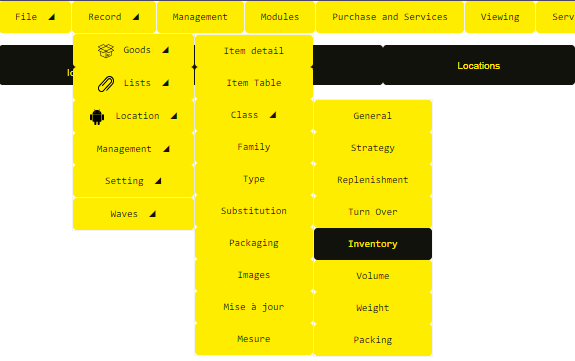
\includegraphics[width=0.8\linewidth]{images/delphi_menu.png}
				\end{center}
				\caption{Menu développé en \gls{delphi}}
				\floatfoot{Source de l'image : capture d'écran}
				\label{fig:delphi_menu}
			\end{figure}
	
			\begin{figure}[ht!]
				\begin{center}
					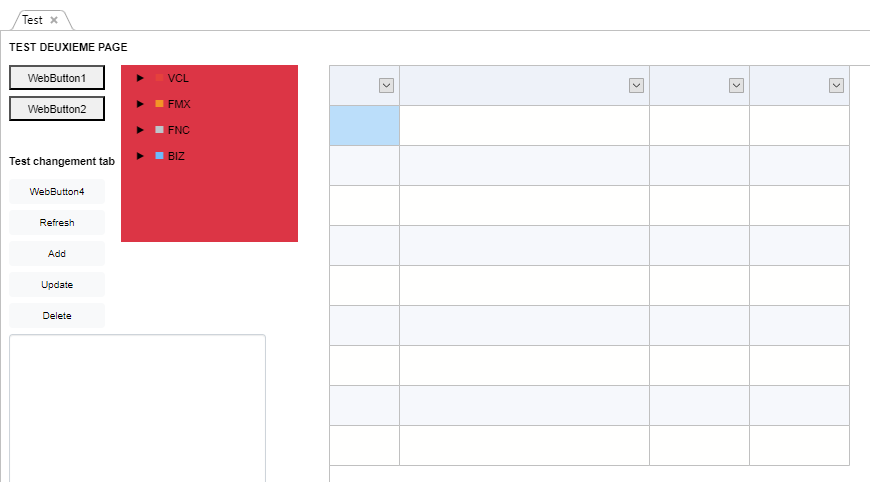
\includegraphics[width=0.8\linewidth]{images/delphi_app.png}
				\end{center}
				\caption{Fenêtre de test développé en \gls{delphi}}
				\floatfoot{Source de l'image : capture d'écran}
				\label{fig:delphi_app}
			\end{figure}
		
		\newpage
		
		\section{Code produit en \gls{delphi}}\label{appendix:delphi_code}
			\begin{figure}[ht!]
				\begin{center}
					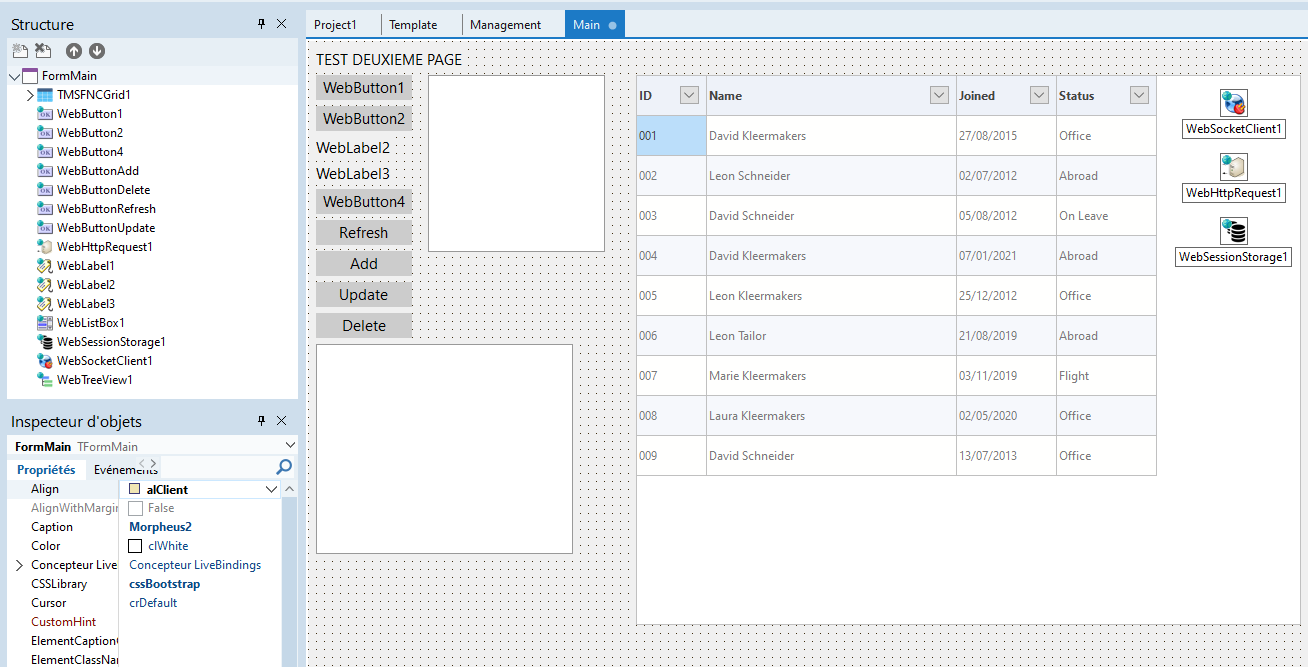
\includegraphics[width=0.9\linewidth]{images/delphi_dev_form.png}
				\end{center}
				\caption{Interface de création de la fenêtre en \gls{delphi}}
				\floatfoot{Source de l'image : capture d'écran}
				\label{fig:delphi_dev_form}
			\end{figure}
	
			\begin{figure}[ht!]
				\begin{center}
					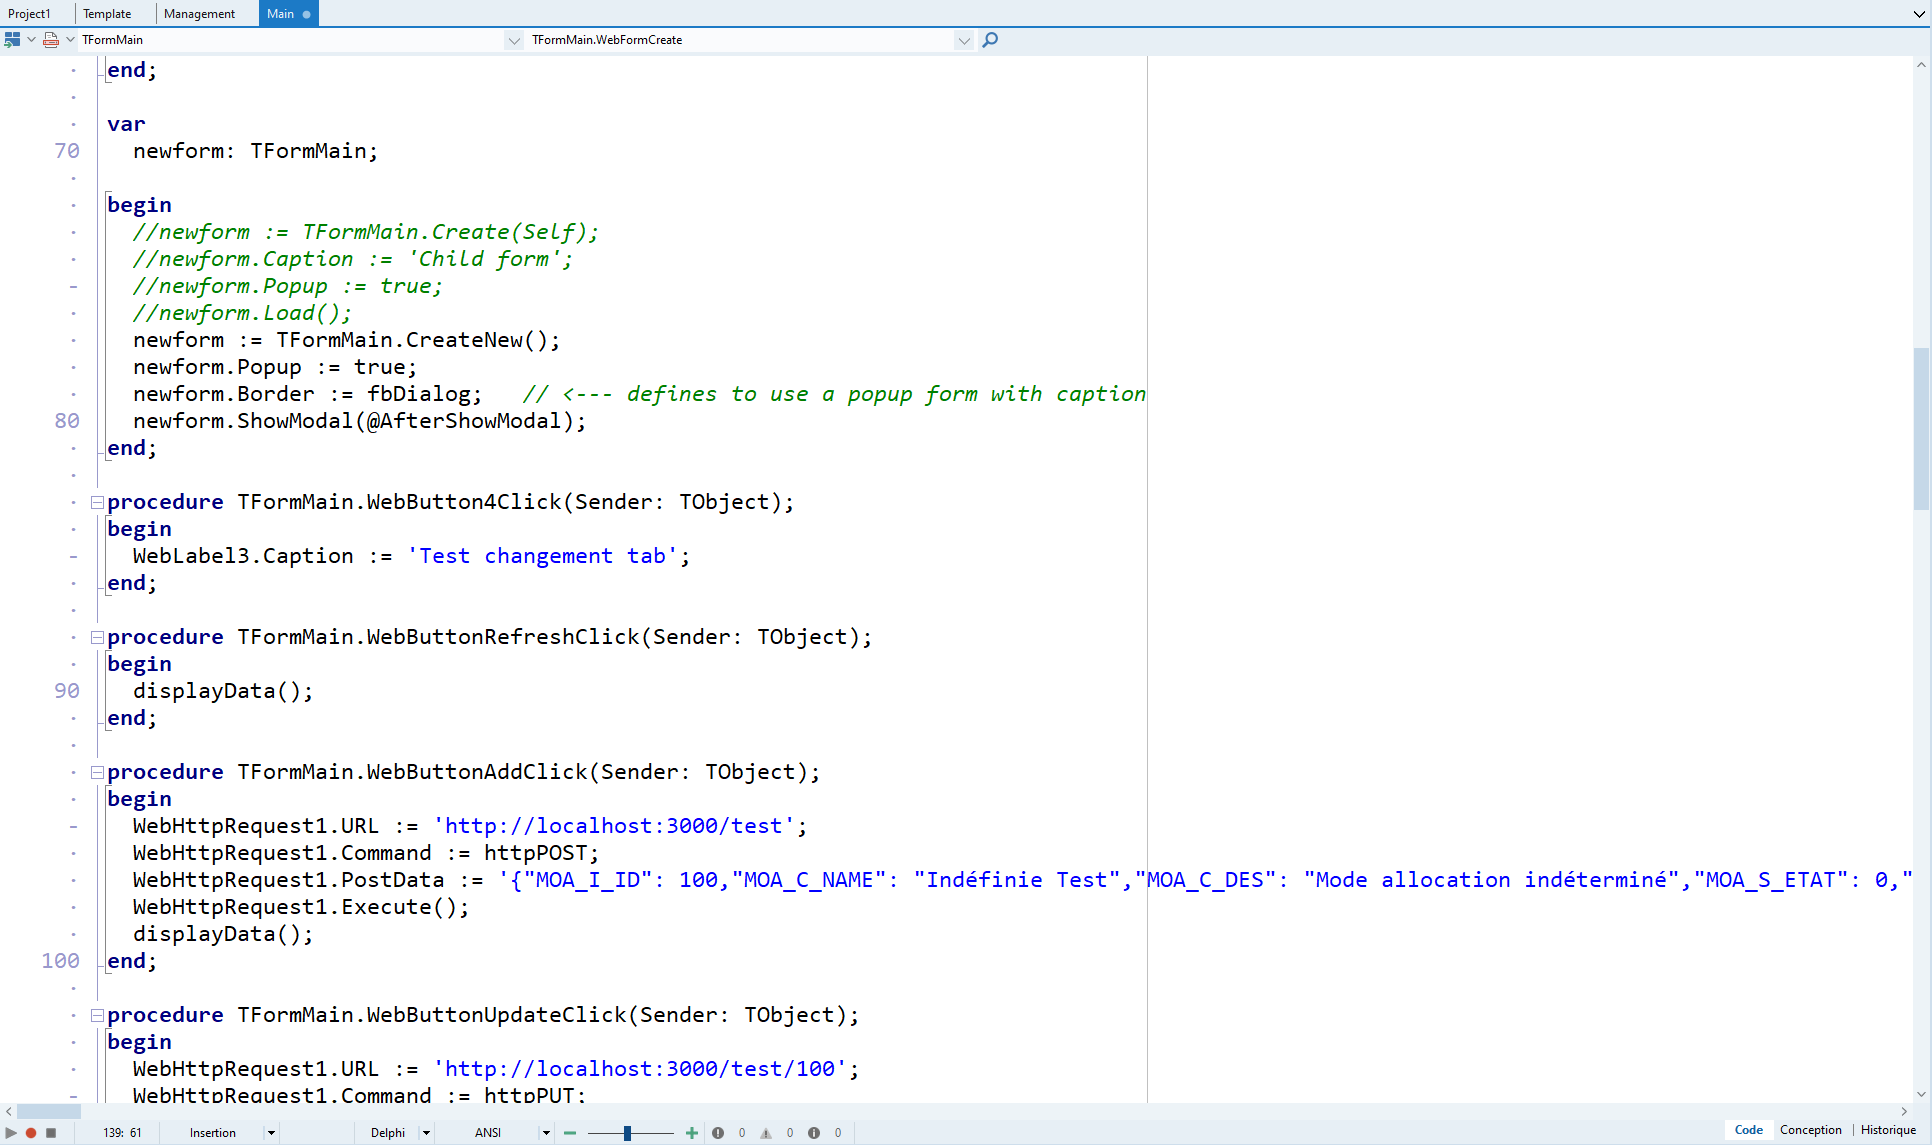
\includegraphics[width=0.9\linewidth]{images/delphi_dev_code.png}
				\end{center}
				\caption{Code associé en \gls{delphi}}
				\floatfoot{Source de l'image : capture d'écran}
				\label{fig:delphi_dev_code}
			\end{figure}

		\newpage

		\section{Code produit en \gls{react} et \gls{devextreme}}\label{appendix:react_code}
			\begin{figure}[h!]
				\begin{center}
					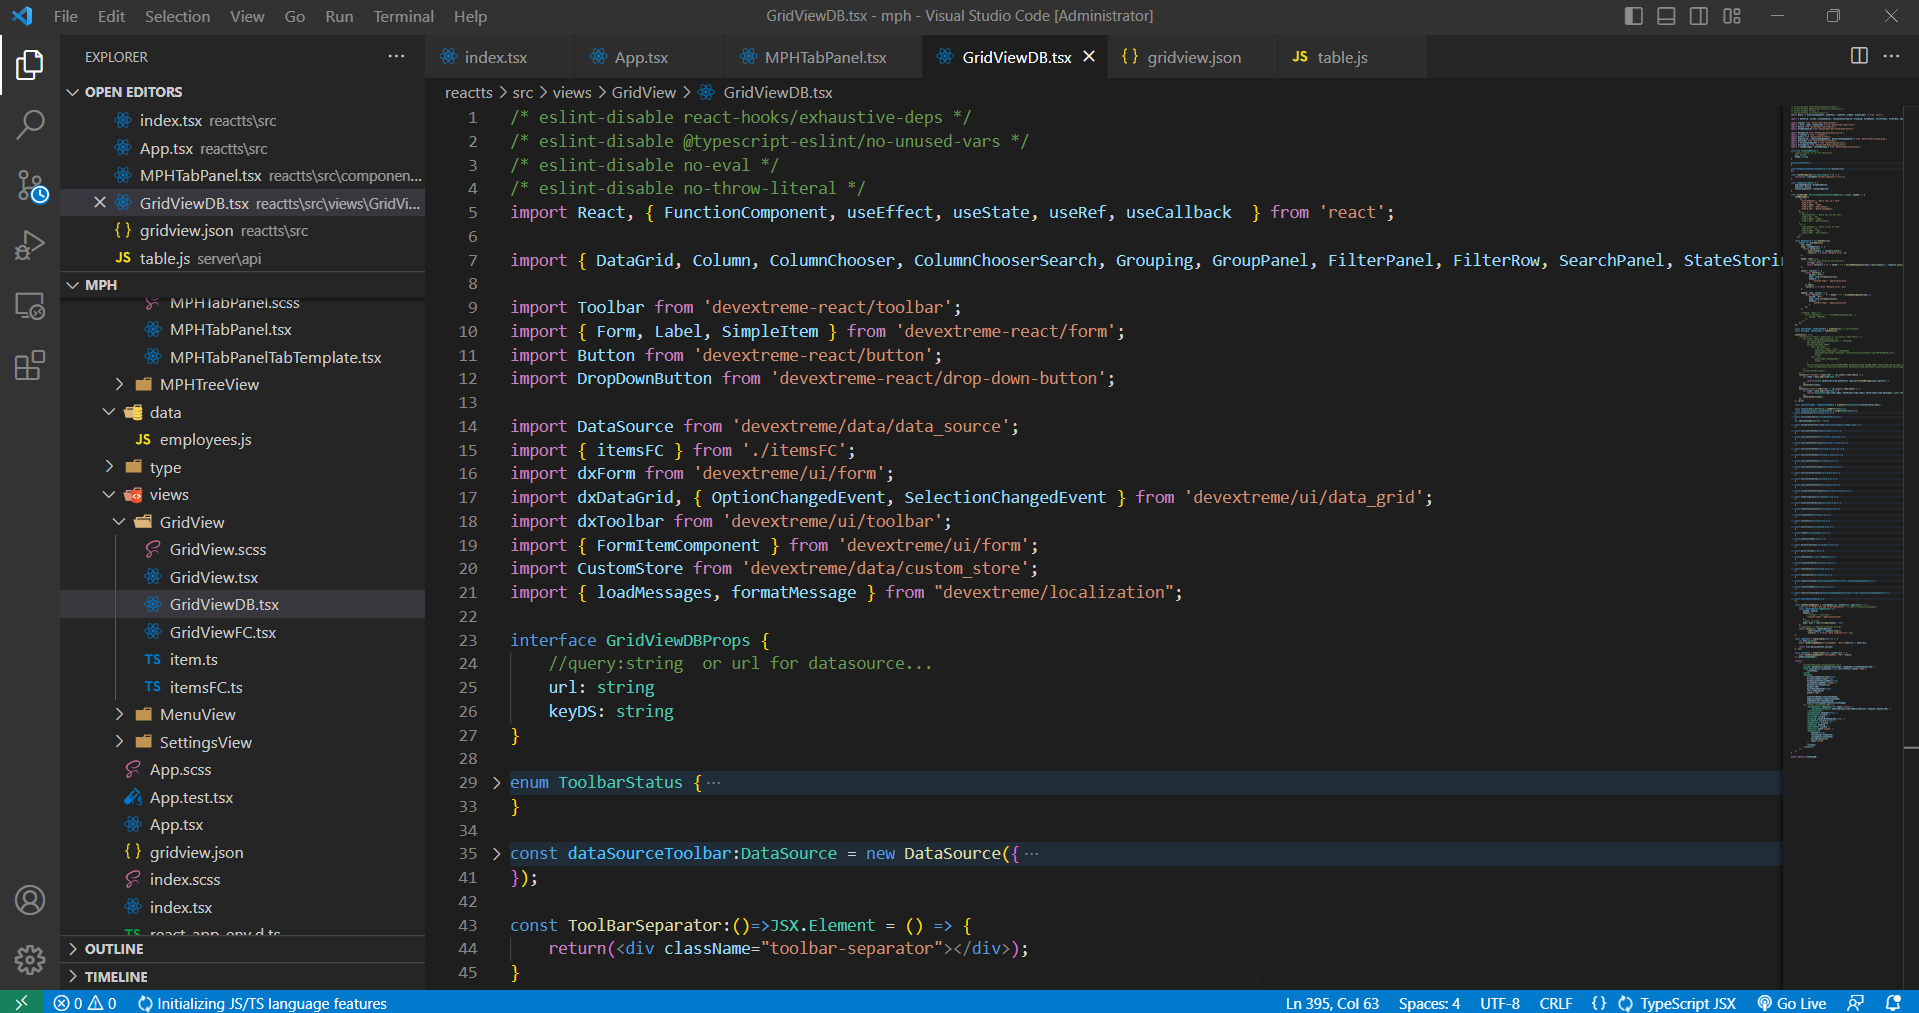
\includegraphics[width=\linewidth]{images/react_code.png}
				\end{center}
				\caption{Exemple de code produit en react}
				\floatfoot{Source de l'image : capture d'écran}
				\label{fig:react_code}
			\end{figure}

		\newpage
		\begin{landscape}
		\section[Comparatif technique entre les solutions \gls{tmsweb} et \gls{devextreme}]{\printSectionFootnote{appendix:tms_devextreme}{methodologie:outils_technologiques:delphi:tms_web, devexpress}}\label{appendix:tms_devextreme}
			\begin{longtable}[c]{p{3cm}|p{8.5cm}|p{8.5cm}}
				\caption{Comparatif technique entre les solutions \gls{tmsweb} et \gls{devextreme}}\\
				\label{tab:tms_devextreme}\\
				\toprule
				\textbf{Critères} & \textbf{\gls{tmsweb}} & \textbf{\gls{devextreme}}\\
				\midrule
				\endfirsthead
				\toprule
				\textbf{Critères} & \textbf{\gls{tmsweb}} & \textbf{\gls{devextreme}}\\
				\midrule
				\endhead
						\hline
						\gls{langage_programmation} & \gls{tmsweb} se base sur le Pascal Objet, un \gls{langage_programmation} \gls{poo}. Il est particulièrement adapté aux développeurs familiers avec \gls{delphi} ou Free Pascal. L'utilisation de Pascal Objet dans \gls{tmsweb} offre une courbe d'apprentissage plus facile pour les développeurs \gls{delphi}. & \gls{devextreme} se base sur \gls{javascript}, un langage incontournable pour le développement web. Cela signifie que les développeurs travaillent directement avec \gls{javascript} et peuvent choisir d'utiliser des \glspl{framework} supplémentaires tels qu'Angular, \gls{react} ou Vue.js pour développer l'application.\\
						\hline
						Composants et widgets & \gls{tmsweb} propose des composants et des widgets basés sur les principes de la \gls{bibliotheque_logicielle} VCL (Visual Component Library) de \gls{delphi}. Cela permet de créer des interfaces riches avec des fonctionnalités avancées. & \gls{devextreme} offre une large gamme de widgets prêts à l'emploi, allant des tableaux de bord interactifs aux graphiques, aux grilles, aux calendriers, etc. Ces widgets sont optimisés pour les performances et l'expérience utilisateur.\\
						\hline
						Intégration et compatibilité & \gls{tmsweb} est étroitement intégré à l'environnement \gls{delphi}. Il est conçu pour être utilisé principalement avec \gls{delphi}, ce qui offre une expérience de développement cohérente pour les utilisateurs existants de \gls{delphi}. Cependant, cela peut limiter la portabilité vers d'autres plates-formes. & \gls{devextreme} est indépendant de la plate-forme et peut être utilisé avec différents environnements de développement tels que Visual Studio Code, Angular, \gls{react}, etc. Cela permet une plus grande flexibilité en termes de choix de la technologie et de la plate-forme.\\
						\hline
						Licence et coûts & Les coûts de \gls{tmsweb} sont souvent associés aux licences \gls{delphi} de \gls{tmssoftware}. Les prix varient en fonction des modules nécessaires et des licences \gls{delphi} choisies. & \gls{devextreme} propose différentes options de licence, y compris une version gratuite pour une utilisation non commerciale. Pour une utilisation commerciale ou l'accès à des fonctionnalités avancées, une licence payante peut être nécessaire.\\
						\hline
						Performance & Les applications \gls{tmsweb} peuvent bénéficier des optimisations et des performances liées à \gls{delphi}. Cependant, étant donné qu'il s'appuie sur le Pascal Objet, il peut y avoir des limites en termes de performances \gls{javascript} (le Pascal Object étant traduit en \gls{javascript}) par rapport aux concurrents \gls{javascript} natifs. & \gls{devextreme} est optimisé pour les performances \gls{javascript} et offre une expérience utilisateur réactive et fluide, en particulier dans les \glspl{app_web} modernes.\\
						\hline
						Documentation et communauté & \gls{tmsweb} dispose d'une documentation et d'une communauté pour soutenir les développeurs, bien que la communauté soit potentiellement plus restreinte que celle des grands \glspl{framework} \gls{javascript}. & \gls{devextreme} bénéficie du soutien de \gls{devexpress}, une entreprise bien établie, et propose une documentation complète et une communauté de développeurs \gls{javascript} active et étendue.\\
				\bottomrule	
			\end{longtable}
		\end{landscape}
		\newpage

		\section{Traduction de la partie Conclusion}\label{appendix:conclusion_translation}
			En conclusion, ce mémoire a exploré en partie le processus complexe et significatif de la transition d'une application \gls{client_lourd} vers une \gls{app_web}. À travers notre étude, nous avons abordé divers aspects techniques, organisationnels et stratégiques de ce passage, mettant en évidence les défis et les opportunités inhérents à cette évolution.\\

		Nous avons d'abord examiné le contexte de cette transition, en présentant l'entreprise SSI SCHÄFER et en définissant les raisons et les motivations qui l'ont poussée à entreprendre cette transformation majeure. Ensuite nous avons posé le cadre théorique du mémoire, ce qui a permis de définir les concepts clés qui ont été présents tout au long du document. Nous avons également effectué une analyse comparative entre les \glspl{app_web} et les applications \gls{client_lourd} afin de mieux comprendre les différences significatives entre les deux approches.\\

		Nous avons ensuite présenté le projet et avons exploré les enjeux et importances qu'il avait pour l'entreprise. Nous sommes ensuite revenus sur la méthodologie et les outils utilisés au cours du projet. Nous avons ainsi mis en évidence l'importance de la planification et de la gestion de projet ainsi que la collaboration et la communication. Cela nous a aussi permis de présenter les outils technologiques utilisés.\\

		Par la suite, nous avons détaillé les étapes clés du processus de migration, en insistant sur la planification stratégique, le choix des technologies, et le développement d'une première version de l'\gls{app_web}. Nous avons mis en évidence l'importance cruciale de la collaboration interdisciplinaire entre les parties prenantes pour assurer le contrôle et le suivi du projet afin de garantir le succès de la transition. Nous avons pu, à travers la cyberattaque qu'a subi l'entreprise, avoir une vision de la gestion d'une crise.\\

		Enfin, nous avons examiné les résultats concrets de la transition, en mettant en évidence les améliorations fonctionnelles. Nous avons également identifié les enseignements clés tirés de cette expérience, notamment l'importance de la planification minutieuse, de la communication transparente et de l'adaptabilité face aux défis imprévus. J'ai aussi pu mette en avant toutes les compétences que j'ai pu utiliser, acquérir et développer au cours de mon stage et qui me serviront de piliers pour mon futur professionnel.\\

		En somme, ce mémoire a démontré que la transition d'une application \gls{client_lourd} à une \gls{app_web} est un processus complexe mais essentiel pour rester compétitif dans un environnement numérique en constante évolution. Il a également souligné l'importance de l'alignement stratégique, de l'engagement des équipes, et de l'analyse approfondie des coûts et des avantages. Cette expérience nous a montré que, avec une planification soignée et une exécution efficace, une entreprise peut réussir à franchir ce cap avec succès et à s'adapter aux nouvelles exigences du marché.\\

		En fin de compte, ce mémoire a été bien plus qu'une simple étude de cas technique, il a été une plongée profonde dans le monde en constante évolution de la technologie, de la gestion de projet, de la communication interdisciplinaire, et de l'adaptabilité aux changements. De plus ce mémoire ne se limite pas à documenter une transition technologique, il nous rappelle que dans le monde en constante évolution d'aujourd'hui, l'adaptabilité, la planification stratégique et la persévérance sont des atouts inestimables pour toute entreprise.\\

		À l'instar de SSI SCHÄFER, nous sommes tous confrontés à la nécessité de nous adapter et d'innover pour prospérer. Les leçons tirées de cette expérience sont autant de boussoles qui peuvent nous guider dans notre propre voyage vers l'avenir numérique.\\

		Alors que nous tournons la dernière page de ce mémoire, gardons à l'esprit que notre exploration ne fait que commencer. Le monde de la technologie continue d'évoluer, les défis émergent de manière inattendue, et les opportunités se présentent à ceux qui sont prêts à les saisir. La transition d'une application \gls{client_lourd} à une \gls{app_web} n'est qu'un chapitre dans l'histoire en constante évolution de l'innovation et de l'adaptation.

		\newpage

	\phantomsection
	\part*{Mots clés}
	%\addcontentsline{toc}{part}{Mots clés}
		\section*{Mots clés}
		\addcontentsline{toc}{section}{Mots clés}
			\noindent Liste des mots clés : delphi, développement web, logistique, Cholet, WMS, WCS, MORPHEUS, tms, react, nodejs, devexpress

		\section*{Keywords}
		\addcontentsline{toc}{section}{Keywords}
			\noindent List of keywords : delphi, web development, logistic, Cholet, WMS, WCS, MORPHEUS, tms, react, nodejs, devexpress

		\section*{Schlüsselwörter}
		\addcontentsline{toc}{section}{Schlüsselwörter}
			Liste der Schlüsselwörter: delphi, web enwicklung, logistik, Cholet, WMS, WCS, MORPHEUS, tms, react, nodejs, devexpress
	\newpage

	\phantomsection
	\part*{Résumés}
	%\addcontentsline{toc}{part}{Résumés}
		\section*{Résumé}
		\addcontentsline{toc}{section}{Résumé}
			Ce mémoire explore la transition des applications \gls{client_lourd} vers des \glspl{app_web}, en se basant sur mon expérience personnelle lors de mon stage chez SSI SCHÄFER. Après avoir présenté l'entreprise SSI SCHÄFER, acteur mondial dans la logistique et entreprise d'accueil du stage, nous avons pu poser le cadre théorique qui couvre des concepts clés tels que les applications \gls{client_lourd}, les \glspl{app_web}, les \gls{frontend} et \gls{backend}, les \glspl{framework}, les \acrshort{api}, et \acrshort{rest}.\\

			La partie scientifique analyse les avantages et inconvénients de ces deux types d'applications, en mettant en évidence que le choix dépend du contexte et des besoins de l'entreprise. Le projet principal avait pour objectif de développer une \gls{app_web} pour rendre le logiciel Morpheus accessible via un navigateur web.\\

			La méthodologie et les outils ont joué un rôle crucial dans le projet, avec l'utilisation d'un modèle en V, de diagrammes de GANTT, de Confluence, et de nombreux outils technologiques. Le projet a suivi diverses étapes, avec un suivi et un contrôle réguliers. Une cyberattaque en avril 2023 a également été observée.\\

			Cela m'a aussi permis de mettre en avant les compétences techniques, en gestion, en communication, en leadership, et en adaptabilité développées pendant le stage, qui sont précieuses pour ma future carrière. Le mémoire conclut en encourageant l'adaptabilité et l'innovation dans un monde technologique en constante évolution.
		
		\section*{Summary}
		\addcontentsline{toc}{section}{Summary}
			This dissertation explores the transition from thick client applications to web applications, based on my personal experience during my internship at SSI SCHAEFER. After presenting the company SSI SCHAEFER, a global player in logistics and host company of the internship, we were able to establish the theoretical \gls{framework} which covers key concepts such as heavy client applications, web applications, \gls{frontend} and \gls{backend}, \glspl{framework}, \acrshort{api}s, and \acrshort{rest}.\\

			The scientific part analyzes the advantages and disadvantages of these two types of applications, highlighting that the choice depends on the context and the needs of the company. The main project aimed to develop a web application to make the Morpheus software accessible via a web browser.\\

			The methodology and tools played a crucial role in the project, with the use of a V-model, GANTT charts, Confluence, and numerous technological tools. The project followed various stages, with regular monitoring and monitoring. A cyberattack in April 2023 was also observed.\\

			It also allowed me to highlight the technical, management, communication, leadership, and adaptability skills developed during the internship, which are valuable for my future career. The dissertation concludes by encouraging adaptability and innovation in an ever-changing technological world.

		\section*{Zusammenfassung}
		\addcontentsline{toc}{section}{Zusammenfassung}
			Diese Dissertation untersucht den Übergang von Thick-Client-Anwendungen zu Webanwendungen, basierend auf meiner persönlichen Erfahrung während meines Praktikums bei SSI SCHÄFER. Nach der Vorstellung des Unternehmens SSI SCHÄFER, einem Global Player in der Logistik und Gastgeberunternehmen  des Praktikums, konnten wir den theoretischen Rahmen festlegen, der Schlüsselkonzepte wie Heavy-Client-Anwendungen, Webanwendungen, \Gls{frontend} und \Gls{backend}, \Glspl{framework}, \acrshort{api}s und \acrshort{rest} umfasst.\\

			Der wissenschaftliche Teil analysiert die Vor- und Nachteile dieser beiden Arten von Anwendungen und betont, dass die Wahl vom Kontext und den Bedürfnissen des Unternehmens abhängt. Das Hauptprojekt zielte darauf ab, eine Webanwendung zu entwickeln, um die Morpheus- Software über einen Webbrowser zugänglich zu machen.\\

			Die Methodik und die Tools spielten mit der Verwendung eines V-Modells, GANTT-Diagrammen, Confluence sowie zahlreichen technologischen Tools im Projekt eine entscheidende Rolle. Das Projekt verlief in verschiedenen Phasen mit regelmäßiger Überwachung und Kontrolle. Auch ein Cyberangriff im April 2023 wurde beobachtet.\\

			Dadurch konnte ich auch die technischen, Management-, Kommunikations-, Führungs- und Anpassungsfähigkeiten hervorheben, die ich während des Praktikums entwickelt habe und die für meine zukünftige Karriere wertvoll sind. Die Dissertation schließt mit der Förderung von Anpassungsfähigkeit und Innovation in einer sich ständig verändernden technologischen Welt.  


\end{document}